\documentclass[11pt]{book}
\usepackage[]{authblk}
\usepackage{graphicx}
\usepackage{tabularx}
%\usepackage{color}
\usepackage{colortbl}
\usepackage[usenames,dvipsnames,table]{xcolor}
\usepackage{booktabs}
\usepackage{longtable}
\usepackage{hanging}
\usepackage{indentfirst}
\usepackage{setspace}
\usepackage{enumitem}
\usepackage{verbatim}
\usepackage{upgreek}
\usepackage{framed}
\usepackage{ textcomp }
\usepackage{url}
\usepackage{soul}
\usepackage{amsmath, amsfonts,amssymb,mathrsfs}
\usepackage{fancyhdr}
\usepackage[compact]{titlesec}
\usepackage[T1]{fontenc}
\usepackage{lmodern}
\usepackage{float}
\usepackage[caption = false]{subfig}
\usepackage{fancybox}
\usepackage{fixltx2e}

%\usepackage[backend=bibtex,hyperref=true,citestyle=authoryear,bibstyle=authortitle,firstinits=true,terseinits=true,doi=false,url=false,maxbibnames=10,maxcitenames=2]{biblatex}
%\addbibresource{../bib_tex/master_refs.bib}


\usepackage[sectionbib]{chapterbib}
\usepackage[sectionbib]{natbib}

%\input{../bib_tex/biblatex_macros}


\setlength{\evensidemargin}{0in}
\setlength{\headheight}{0in}
\setlength{\headsep}{0in}
\setlength{\oddsidemargin}{-0.25in}
\setlength{\paperheight}{11in}
\setlength{\paperwidth}{8.5in}
\setlength{\tabcolsep}{0in}
\setlength{\textheight}{9in}
\setlength{\textwidth}{7in}
\setlength{\topmargin}{0in}
\setlength{\topskip}{0in}
\setlength{\voffset}{0in}
\parskip = 0.15in
\pagestyle{plain}
\setlength{\parindent}{0cm}

\definecolor{citescol}{RGB}{60,179,113}
\definecolor{urlscol}{RGB}{0,150,206}
\definecolor{linkscol}{RGB}{34,139,34}
\definecolor{mycol}{RGB}{25,23,191}
\definecolor{outputcol}{RGB}{34,139,34}
\definecolor{tcol}{RGB}{165,0,14}


\DeclareMathAlphabet{\msfsl}{T1}{cmr}{m}{it}
\DeclareMathAlphabet{\msyf}{OMX}{pcr}{m}{it}
\newcommand{\alf}{\upalpha}
\newcommand{\hilight}[1]{\colorbox{yellow}{#1}}

\newcommand{\levelone}[1]{
\bigskip
\noindent{\LARGE{\textsc{#1}}}
\vspace {0.05in}
}

\newcommand{\leveltwo}[1]{
\bigskip
\noindent{\Large{\textit{#1}}}
\vspace {-1mm}
}

\newcommand{\descriptionhead}[1]{
\noindent{\textbf{\textit{#1}}}\\ \vspace{-7mm}
}

\newcommand{\dhead}[1]{
\noindent{\textbf{\textit{#1 --}}}
}


\newcommand{\exs}[1]{
\vspace{-4mm}
\begin{itemize}
\item #1 \\ \vspace{-8mm}
\end{itemize}
}

\newcommand{\nbo}[1]{{\color{red}{#1}}}


\newcommand{\stepbullet}{\noindent \textbullet \ }
\newcommand{\mi}[1]{\textbf{\textit{#1}}}


\newcommand{\levelthree}[1]{\textit{#1 --}}


%\bibliographystyle{apalike}
%\bibpunct[; ]{(}{)}{;}{a}{,}{;}

\usepackage[breaklinks,pdfhighlight ={/N}]{hyperref}
\usepackage[all]{hypcap}
\hypersetup{colorlinks=true,linkcolor=linkscol,citecolor=citescol,urlcolor=urlscol}


% Abbreviations
\usepackage{xspace}
\newcommand{\IE}{{\it i.e.,}\xspace}
\newcommand{\EG}{{\it e.g.,}\xspace}
\newcommand{\CF}{{\it cf.}\xspace}
\newcommand{\IID}{i.i.d.\xspace}

\newcommand{\BAMM}{\texttt{BAMM}\xspace}
\newcommand{\BEAST}{\texttt{BEAST}\xspace}
\newcommand{\BiSSE}{\texttt{BiSSE}\xspace}
\newcommand{\DDD}{\texttt{DDD}\xspace}
\newcommand{\diversitree}{\texttt{diversitree}\xspace}
\newcommand{\FigTree}{\texttt{FigTree}\xspace}
\newcommand{\HiSSE}{\texttt{HiSSE}\xspace}
\newcommand{\Laser}{\texttt{laser}\xspace}
\newcommand{\MrBayes}{\texttt{MrBayes}\xspace}
\newcommand{\PAML}{\texttt{PAML}\xspace}
\newcommand{\PBD}{\texttt{PBD}\xspace}
\newcommand{\PhyloBayes}{\texttt{PhyloBayes}\xspace}
\newcommand{\Phylowood}{\texttt{Phylowood}\xspace}
\newcommand{\R}{\texttt{R}\xspace}
\newcommand{\Rev}{\texttt{Rev}\xspace}
\newcommand{\RevBayes}{\texttt{RevBayes}\xspace}
\newcommand{\RevGadgets}{\texttt{RevGadgets}\xspace}
\newcommand{\TESS}{\texttt{TESS}\xspace}
\newcommand{\Tracer}{\texttt{Tracer}\xspace}
\newcommand{\TreePar}{\texttt{TreePar}\xspace}

\newcommand{\COO}{CO\textsubscript{2}\xspace}


\let\otheriint\iint
\let\iint\relax
\usepackage{ wasysym }

\usepackage{framed}
\usepackage[]{listings}
%\usepackage{fontspec}
\usepackage{placeins}
\usepackage{epstopdf}

\lstset{breaklines=true}

\lstdefinestyle{textboxSmall}{
  language=Matlab,
  stepnumber=1,
  numbersep=10pt,
  tabsize=4,
  showspaces=false,
  showstringspaces=false
}

%\definecolor{shadecolor}{RGB}{238,224,229}
%\definecolor{shadecolor}{RGB}{135,206,250}
\definecolor{shadecolor}{RGB}{183,207,237}

%\definecolor{TextFieldBackgroundColor}{rgb}{0.56, 0.74, 0.56}
\definecolor{TextFieldBackgroundColor}{rgb}{.85 .85 .85}
%\definecolor{TextFieldBoxColor}{RGB}{0.56, 0.74, 0.56}
\definecolor{TextFieldBoxColor}{RGB}{1, 1, 1}
\definecolor{TextFieldTextColor}{RGB}{0, 0, 0}
\newcommand{\TextFieldWidth}{0.92\textwidth}

\setlength{\tabcolsep}{5pt}
\setlength{\topmargin}{-0.4in}
\setlength{\headheight}{14.5pt}
\pagestyle{fancy}


\newcommand{\forceindent}{\leavevmode{\parindent=25pt\indent}}

\newcommand{\taha}[1]{{\textcolor{red}{[TAH comment: #1]}}} % TAH comment

\titlespacing{\section}{0pt}{*0}{*0}
\titlespacing{\subsection}{0pt}{*0}{*0}
\titlespacing{\subsubsection}{0pt}{*0}{*0}

\titleformat{\section}
  {\normalfont\Large\bfseries\color{mycol}}
  {\thesection}{1em}{}

\titleformat{\subsection}
  {\normalfont\large\bfseries\color{mycol}}
  {\thesubsection}{1em}{}

\titleformat{\subsubsection}
  {\normalfont\bfseries\color{mycol}}
  {\thesubsubsection}{1em}{}

% command for MrBayes command-line step
\newcommand{\cl}[1]{{\texttt{\textbf{#1}}}}

\newcommand{\colx}[1]{{\textcolor{tcol}{#1}}}

\newcommand{\rbprmt}{ > } 
\newcommand{\rbcl}[1]{\exs{\cl{\rbprmt{#1}}}}
\newcommand{\rbout}[1]{\cl{\textcolor{outputcol}{#1}}}
\newcommand{\rbdn}{{\Large \symbol{126}}} % This makes a copy/pasteable tilde
\newcommand{\rbclml}[1]{\exs{\cl{\ \ \ \ \ \ \ \ \ \ \ {#1}}}}



% text box settings
% requires compiling w/ XeLaTeX
%\newfontfamily\listingsfont[Scale=1.0]{Courier New}
%\lstset{basicstyle=\listingsfont, columns=texcl}
%\defaultfontfeatures{Mapping=tex-text}

%\lstset{columns=fullflexible}
%\lstset{basicstyle=\ttfamily,columns=flexible}
\lstdefinelanguage{Rev}
{morekeywords={RevBayes},
sensitive=false,
morecomment=[l]{\#},
moredelim=[il][\color{gray}\ttfamily]{|*},
}
%\lstdefinelanguage{Rev}
%{morecomment=[l]{#},
%moredelim=[il][\color{gray}\ttfamily]{|*},
%}
\lstset{
    language=Rev,
    basicstyle=\ttfamily,
    columns=flexible
}
%\lstset{morecomment=[l]{\#}}


% Some commands to keep the sysbio.bst from generating weird errors
\newcommand{\bibAnnoteFile}[1]{%
\IfFileExists{#1}{\begin{quotation}\noindent\textsc{Key:} #1\\
\textsc{Annotation:}\ \input{#1}\end{quotation}}{}}

\newcommand{\bibAnnote}[2]{%
\begin{quotation}\noindent\textsc{Key:} #1\\
\textsc{Annotation:}\ #2\end{quotation}}

\bibliographystyle{sysbio}
\bibpunct[; ]{(}{)}{;}{a}{}{;}



\makeatletter
\lst@CCPutMacro\lst@ProcessOther {"2D}{\lst@ttfamily{-{}}{-{}}}
\@empty\z@\@empty
\makeatother

% commands
\newcommand{\impmark}{\strut\vadjust{\domark}}
\newcommand{\domark}{%
  \vbox to 0pt{
    \kern-\dp\strutbox
    \smash{\llap{$\rightarrow$\kern1em}}
    \vss
  }%
}



%\usepackage[square,numbers,sectionbib]{natbib}
%\usepackage{chapterbib}
%\usepackage[sectionbib]{natbib}
%\usepackage{biblatex}

%\usepackage[backend=bibtex,hyperref=true,citestyle=authoryear,bibstyle=authortitle,firstinits=true,terseinits=true,doi=false,url=false,maxbibnames=10,maxcitenames=2]{biblatex}
%\addbibresource{../bib_tex/master_refs.bib}
%\input{../bib_tex/biblatex_macros}


\begin{document}
\renewcommand{\headrulewidth}{0.5pt}
\headsep = 20pt
\lhead{ }
\rhead{\textsc {RevBayes Manual}}

%\thispagestyle{plain}

\title{\Huge \textbf{Statistical Phylogenetic Inference using RevBayes} }
\author{
Sebastian H{\"o}hna,
%\and
Tracy A. Heath,
%\and
Michael J. Landis,
%\and
Bastien Boussau,
%\and
Nicolas Lartillot,
%\and
Brian R. Moore,
%\and
Fredrik Ronquist, and
%\and
John P. Huelsenbeck
}


\maketitle

\tableofcontents

\def \GlobalResourcePath {./}

\part{Getting Started with RevBayes}

\chapter{Introcution}
\def \ResourcePath {RB_Getting_Started/}

\section{Overview}

\RevBayes has as its central idea that any statistical model, for example a phylogenetic model, is composed of smaller parts that can be decomposed and put back together in a modular fashion. This comes from considering (phylogenetic) models as \textit{probabilistic graphical models}, which lends flexibility and enhances the capabilities of the program. 
Users interact with \RevBayes via an interactive shell.
Users communicate commands using a language specifically designed for \RevBayes, called \Rev; an R-like language (complete with control statements, user-defined functions, and loops) that enables the user to build up (phylogenetic) models from simple parts (random variables, variable/parameter transformations, models, and constants of different sorts).
 
Here we assume that you have successfully installed \RevBayes.
If this isn't the case, then please consult our website on how to install \RevBayes.



\bigskip
\section{Getting Started}

For the examples outlined in each tutorial, we will use \RevBayes interactively by typing commands in the command-line console.
For the exercises you can either use \RevBayes interactively or run an entire script.
Execute the \RevBayes binary. If this program is in your path, then you can simply type in your Unix terminal:

\exs{\cl{\$ rb}}

When you execute the program, you will see a brief program information, including the current version number. 
Remember that more information can be obtained from \href{www.RevBayes.com}{www.RevBayes.com}.
When you execute the program with an additional filename, \EG
\exs{\cl{\$ rb my\_analysis.Rev}}
then \RevBayes will run all commands specified in your file.

You may want to run \RevBayes in parallel using multiple processes.
This can be done by starting \RevBayes with
\exs{\cl{\$ mpirun -np 4 rb-mpi}}
which starts 4 processes of \RevBayes.
You may want to change the number of processes depending on your available hardware.

The format of the exercises uses \colorbox{shadecolor}{\tt blue shaded boxes} to delineate code examples that you should type into \RevBayes. 
For example, after opening the \RevBayes program, you can load your data file:
{\tt \begin{snugshade*}
\begin{lstlisting}
data <- readDiscreteCharacterData("data/primates_cytb.nex")
\end{lstlisting}
\end{snugshade*}}

%Multi-line entries, particularly loops, will often be displayed in boxes.
The \cl{RevBayes >} prompt that you see in your terminal is omitted so that the examples can be copied and pasted wholly. 
This is especially useful for larger command blocks, particularly loops, which will often be displayed in boxes
{\tt \begin{snugshade*}
\begin{lstlisting}
for( i in 1:12 ){
  x[i] ~ dnExponential(1.0)
}
\end{lstlisting}
\end{snugshade*}}

The various \RevBayes commands and syntax within the text are specified using \cl{typewriter text}. 

Most tutorials also includes hyperlinks: bibliographic citations are {\textcolor{citescol}{medium sea green}} and link to the full citation in the references, external URLs are {\textcolor{urlscol}{cerulean}}, and internal references to figures and equations are {\textcolor{linkscol}{forest green}}.

The various exercises in this tutorial take you through the steps required to perform phylogenetic analyses of the example datasets. 
In addition, we have provided the \Rev scripts and output files for some exercises so you can verify your results.
(Note that since the MCMC runs you perform will start from different random seeds, the output files resulting from your analyses \textit{will not} be identical to the ones we provide you.)


\bigskip
\section{Probabilistic Graphical Models}

\RevBayes uses \textit{probabilistic graphical models} for model specification, visualization, and implementation \citep{Hoehna2014b}. 
Graphical models are frequently used in machine learning and statistics to conceptually represent the conditional dependence structure of complex statistical models with many parameters \citep{Gilks1994,Lunn2000,Jordan2004,Koller2009,Lunn2009}. 
The graphical model framework allows for flexible model specification and implementation and reduces redundant code. 
This framework provides a set of symbols for depicting a \href{http://en.wikipedia.org/wiki/Directed_acyclic_graph}{\textit{directed acyclic graph}} (DAG). 
\citet{Hoehna2014b} described the use of probabilistic graphical models for phylogenetics. 
The different nodes and components of a phylogenetic graphical model are shown in Figure \ref{gmnotation} \citep[Fig. 1 from][]{Hoehna2014b}. 
\begin{figure}[h!]
\centering
\fbox{\includegraphics[width=1.8in,angle=0]{\ResourcePath figures/GM_notation_figure.eps}}
\caption{\small The symbols for a visual representation of a graphical model. 
a) Solid squares represent constant nodes, which specify fixed-valued variables. 
b) Stochastic nodes are represented by solid circles. 
These variables correspond to random variables and may depend on other variables. 
c) Deterministic nodes (dotted circles) indicate variables that are determined by a specific function applied to another variable. 
They can be thought of as variable transformations. 
d) Observed states are placed in clamped stochastic nodes, represented by gray-shaded circles. e) Replication over a set of variables is indicated by enclosing the replicated nodes in a plate (dashed rectangle). 
[Partially reproduced from Fig.~1 in \citet{Hoehna2014b}.]
}
\label{gmnotation}
\end{figure}

To represent the DAG, nodes are connected with arrows indicating dependency. 
A simple, albeit abstract, graphical model is shown in Figure \ref{simpleGM}. 
In this model, we observe a set of states for parameter $x$. 
We assume that the values of $x$ are samples from a lognormal distribution with a location parameter (log mean) $\mu$ and a standard deviation $\sigma$. 
It is more straightforward to model our uncertainty in the expectation of a lognormal distribution, rather than $\mu$, thus we place a gamma distribution on the mean $M$. 
This gamma hyperprior has two parameters that we specify with fixed values (constant nodes): the shape $\alpha$ and rate $\beta$. 
The variable $M$ is a stochastic node with this prior density.
The standard deviation, $\sigma$, is also a stochastic node with an exponential prior density with rate parameter $\lambda$.
For any value of $M$ and any value of $\sigma$ we can compute the deterministic variable $\mu$ using the formula $\mu = \ln(M) - \frac{\sigma^2}{2}$. 
This formula is known from using simple algebra on the equation for the mean of any \href{http://en.wikipedia.org/wiki/Log-normal_distribution}{lognormal distribution}.
With this model structure, we can then calculate the probability of the data conditional on the model and parameter values (the likelihood): 
$\mathbb{P}(\boldsymbol{x} \mid \mu, \sigma)$. 
Next we can get the posterior probability using Bayes' theorem:
$$\mathbb{P}(M,\sigma \mid \boldsymbol{x}, \alpha, \beta, \lambda) = \frac{\mathbb{P}(\boldsymbol{x} \mid \mu, \sigma) \mathbb{P}(M \mid \alpha,\beta) \mathbb{P}(\sigma \mid \lambda)}{\mathbb{P}(\boldsymbol{x})}.$$
\begin{figure}[h!]
\centering
\fbox{\includegraphics[width=2.5in,angle=0]{\ResourcePath figures/simple_GM.eps}}
\caption{\small Graphical model representation of a simple lognormal model. A total of $N$ observations of variable $x$ are observed and occupy a clamped node. 
This parameter is log-normally distributed with parameters $\mu$ and $\sigma$ (log mean and standard deviation, respectively). 
The parameter $\mu$ is a deterministic node that is calculated from the stochastic nodes $M$ (the mean of the distribution) and $\sigma$. 
Dotted arrows indicate deterministic functions and are used to connect deterministic nodes to their parent variables. 
A gamma distribution is applied as a hyperprior on $M$ with constant nodes for the shape $\alpha$ and rate $\beta$.
The stochastic variable $\sigma$ is exponentially distributed with fixed value for the rate $\lambda$.
}
\label{simpleGM}
\end{figure}



\bigskip
\section{\Rev: The \RevBayes Language}

In \RevBayes models and analyses are specified using an interpreted language called \Rev. 
\Rev bears similarities to the compiled language in WinBUGS and the interpreted \R language. 
Setting up and executing a statistical analysis in \RevBayes requires the user to specify all of the parameters of their model and the type of analysis (\EG an MCMC run). 
By using an interpreted language, \RevBayes enables the practitioner to build complex, hierarchical models and to check the current states of variables while building the model. 
This will be very useful in the beginning.
Later on you, when you run very complex analyses, you may want to write \Rev-scripts.

Differently to \R and BUGS, \Rev is a strongly but implicitly typed language.
It is implicitly typed, and thus similar to Python, because you do not need to provide the type of a variable (which you need to in languages such as C++ and Java).
We do implicit typing to help users who do not know about the actual types of the variables.
However, strongly typed means that every variable has a type and arguments of functions need to match the required types.
The strong type requirements ensures that you build meaningful model graphs. 
For example, the variance parameter of a normal distribution needs to be a positive number, and thus you can only use variables that are positive real numbers.
\RevBayes does automatic type conversion.

\bigskip
\subsection{Specifying Models}

\begin{table}[h!]
\centering
\caption{\Rev assignment operators, clamp function, and plate/loop syntax.}\label{operatorTable}
\begin{tabular}{@{\extracolsep{\fill}}l  c r }
\hline
\multicolumn{1}{l}{\textbf{Operator}} & \multicolumn{1}{c}{ } & \multicolumn{1}{r}{\textbf{Variable}}  \\ 
\hline
\cl{<-} & \hspace{10mm} &  constant variable\\
\cl{\rbdn} & \hspace{10mm} &  stochastic variable\\
\cl{:=} & \hspace{10mm} &  deterministic variable\\
\cl{node.clamp(data)} & \hspace{10mm} &  clamped variable\\
\cl{=} & \hspace{10mm} &  inference (\IE non-model) variable\\
\cl{for(i in 1:N)\{...\}} & \hspace{10mm} &  plate\\
\hline
\end{tabular}
\end{table}

The variables/parameters of a statistical model are created using different operators in \Rev (Table \ref{operatorTable}). 
In Figure \ref{revgmexample}, the \Rev syntax for creating the model in Figure \ref{simpleGM} is provided.
Because \Rev is an interpreted language, it is important to consider the order in which you specify your variables (\CF BUGS where the order is not important). 
Thus, typically the first variables that are instantiated are \emph{constant variables}. 
Constant variables require you to assign a fixed value using the \cl{<-} operator. 
Stochastic variables are initialized using the \cl{\rbdn} operator followed by the constructor function for a distribution. 
In \Rev, the naming convention for distributions is \cl{dn*}, where \cl{*} is a wildcard representing the name of the distribution. 
Each distribution function requires hyperparameters passed in as arguments.
This is effectively linking nodes using arrows in the graphical model.
The following code snippet creates a stochastic variable called \cl{M} which is assigned a gamma-distributed hyperprior, with shape \cl{alpha} and rate \cl{beta}:
{\tt \begin{snugshade*}
\begin{lstlisting}
alpha <- 2.0
beta <- 4.0
M ~ dnGamma(alpha, beta)
\end{lstlisting}
\end{snugshade*}}

The flexibility gained from the graphical model framework and the interpreted language allows you to easily change a model by swapping components. 
For example, if you decide that a bimodal lognormal distribution is a better representation of your uncertainty in \cl{M}, then you can simply change the distribution associated with \cl{M} (after initializing the bimodal lognormal hyperparameters):
{\tt \begin{snugshade*}
\begin{lstlisting}
mean_1 <- 0.5
mean_2 <- 2.0
sd_1 <- 1.0
sd_2 <- 1.0
weight <- 0.5
M ~ dnBimodalLognormal(mean_1, mean_2, sd_1, sd_2, weight)
\end{lstlisting}
\end{snugshade*}}

\Rev does allow you to specify constant-variable values in the distribution constructor function; therefore this also works:
{\tt \begin{snugshade*}
\begin{lstlisting}
M ~ dnBimodalLognormal(0.5, 2.0, 1.0, 1.0, 0.5)
\end{lstlisting}
\end{snugshade*}}
Both ways to specify priors are equivalent.
The only difference is that one code may be more readable than the other.



\begin{figure}[h!]
\centering
\fbox{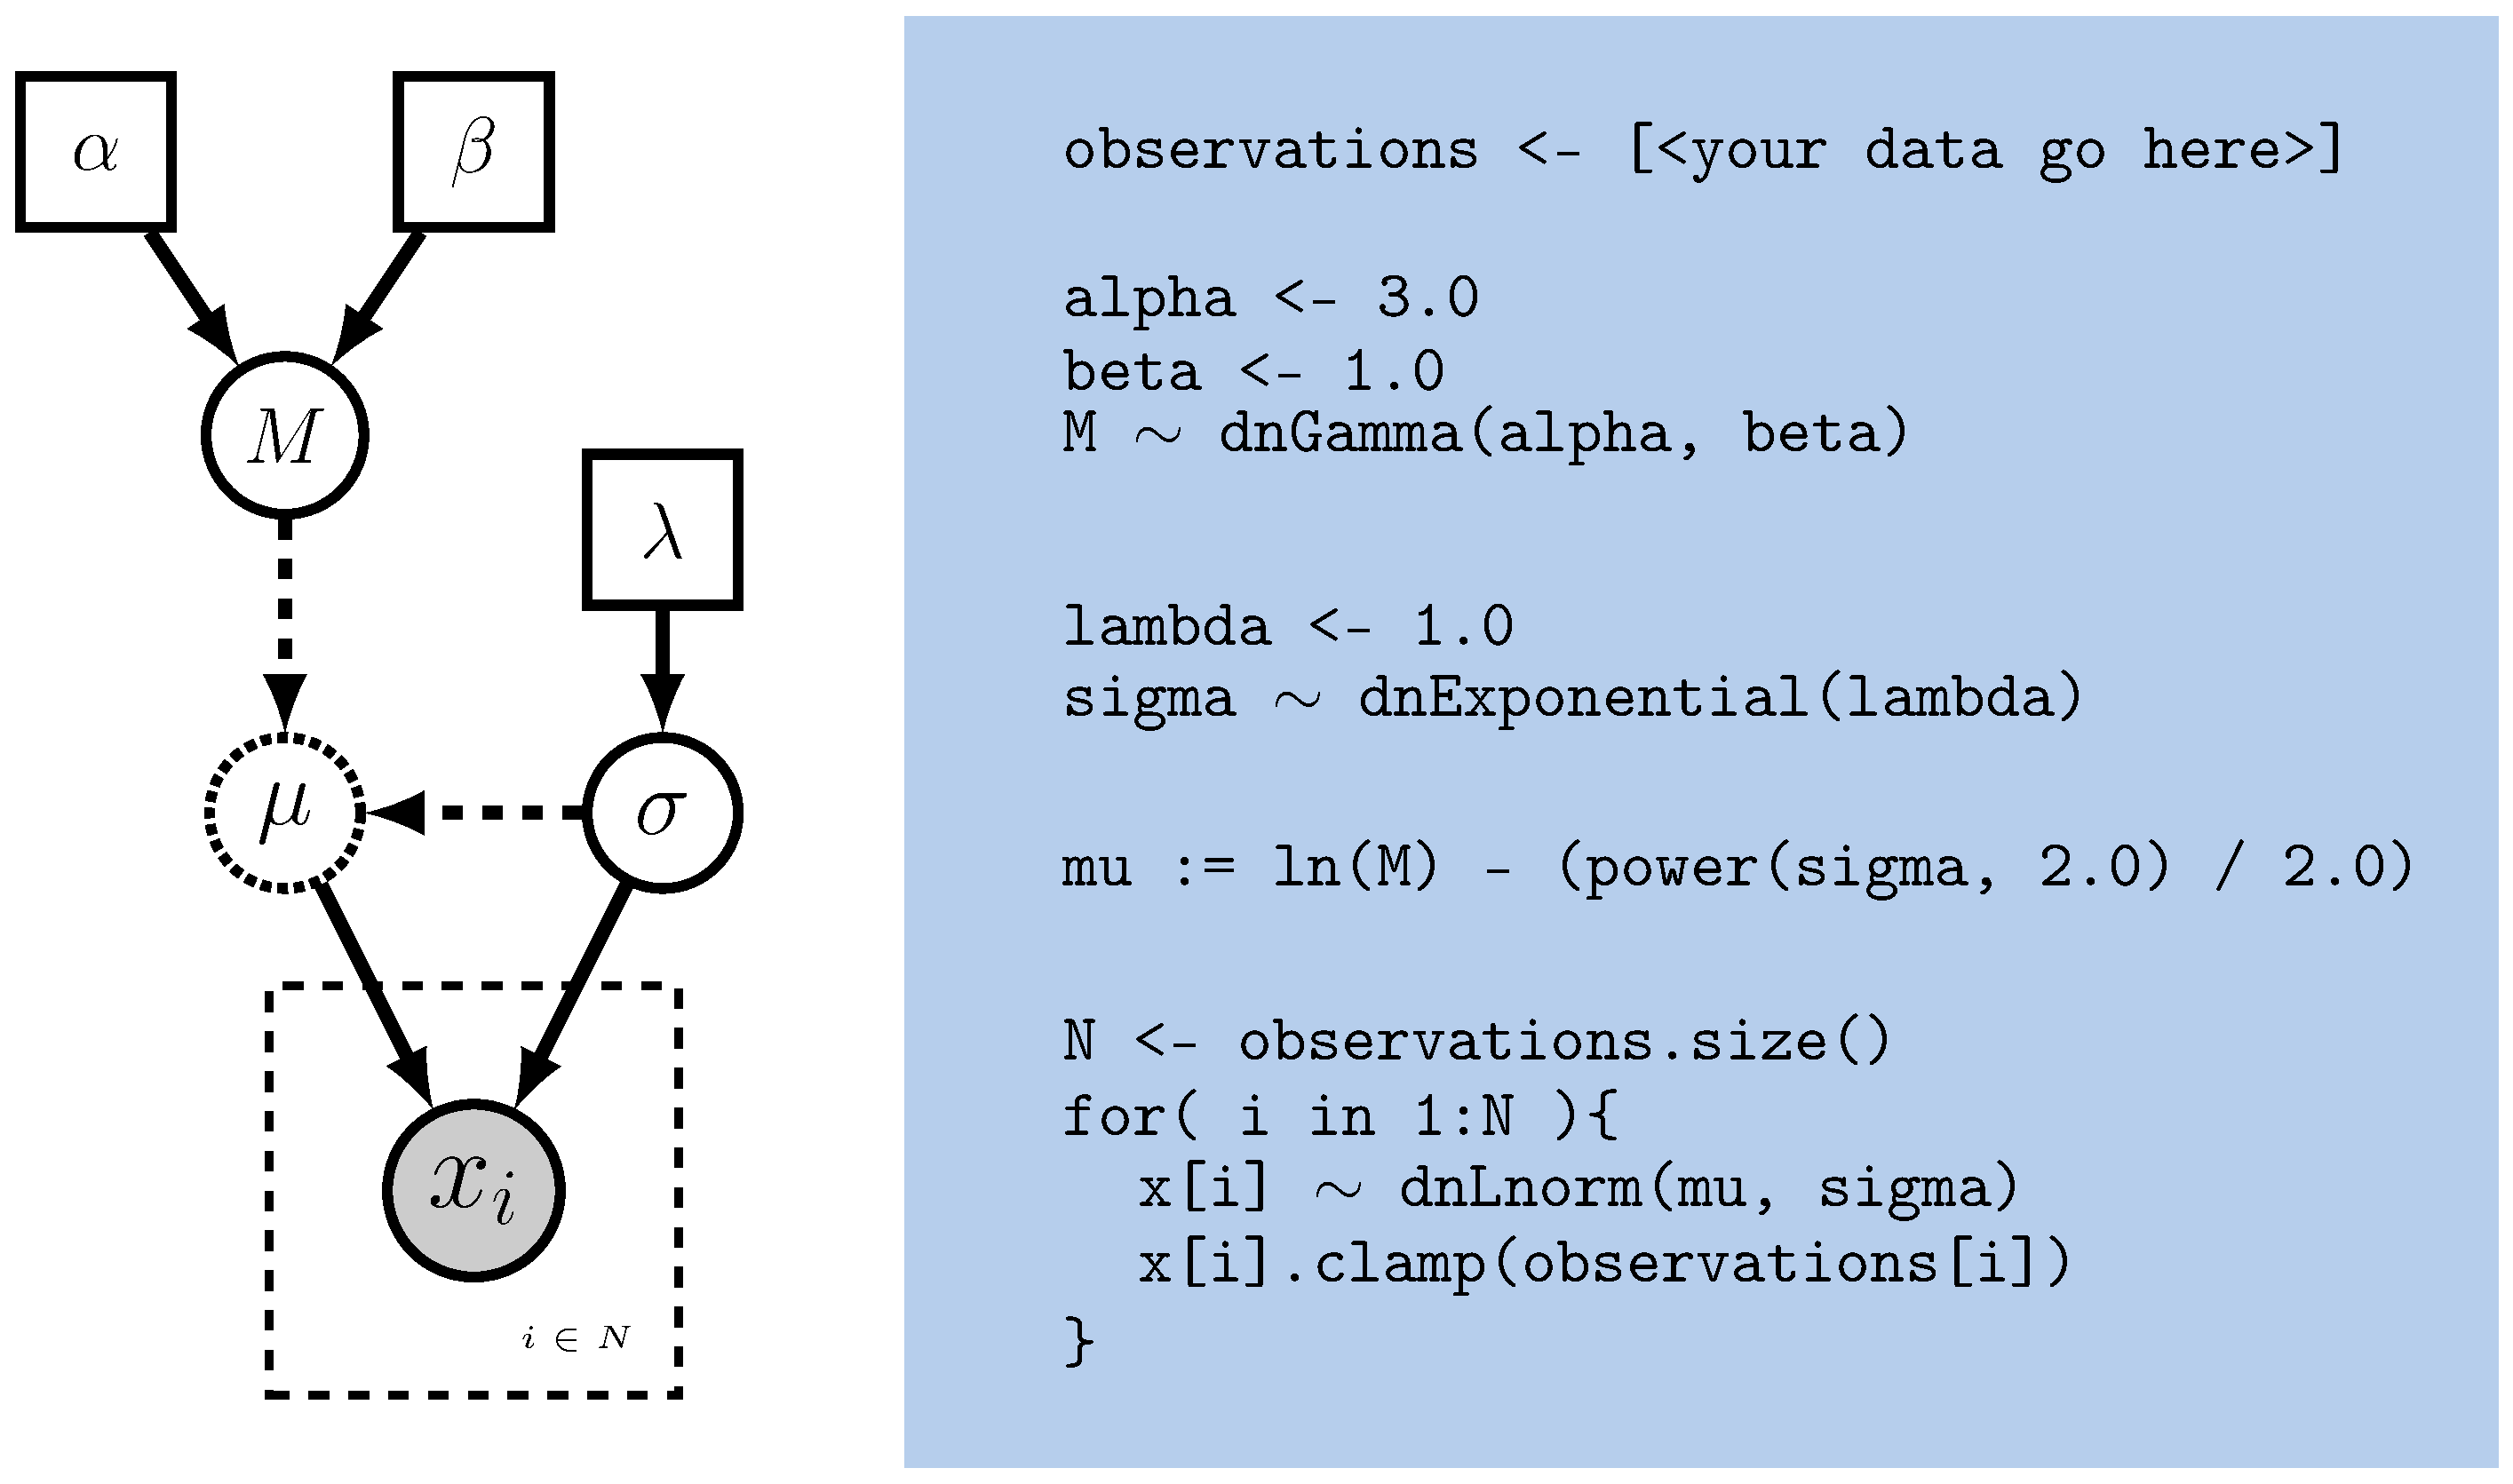
\includegraphics[width=5in,angle=0]{\ResourcePath figures/simple_GM_rev.eps}}
\caption{\small Specifying a model with \Rev. 
The graphical model of the observed parameter $x$ is shown on the left. 
In this example, $x$ is log-normally distributed with a location parameter of $\mu$ and a standard deviation of $\sigma$, thus $x \sim \mbox{Lognormal}(\mu, \sigma)$. 
The expected value of $x$ (or mean) is equal to $M$: $\mathbb{E}(x) = M$. 
In this model, $M$ and $\sigma$ are random variables and each are assigned hyperpriors. 
We assume that the mean is drawn from a gamma distribution with shape parameter $\alpha$ and rate parameter $\beta$: $M \sim \mbox{Gamma}(\alpha, \beta)$. 
The standard deviation of the lognormal distribution is assigned an exponential hyperprior with rate $\lambda$: $\sigma \sim \mbox{Exponential}(\lambda)$. 
Since we are conditioning our model on the \emph{expectation}, we must compute the location parameter ($\mu$) to 
calculate the probability of our model. 
Thus, $\mu$ is a deterministic node that is the result of the function$^*$ executed on $M$ and $\sigma$: $\mu = \ln(M) - \frac{\sigma^2}{2}$. 
Since we observe values of $x$, we \emph{clamp} this node.
}
\label{revgmexample}
\end{figure}

Deterministic variables are parameter transformations and initialized using the \cl{:=} operator followed by the function or formula for calculating the value. 
Previously we created a variable for the expectation of the lognormal distribution.
Now, if you have an exponentially distributed stochastic variable $\sigma$, you can create a deterministic variable for the mean $\mu$:
{\tt \begin{snugshade*}
\begin{lstlisting}
lambda <- 1.0
sigma ~ dnExponential(lambda)
mu := ln(M) - (sigma^2)/2.0
\end{lstlisting}
\end{snugshade*}}

Replication over lists of variables as a plate object is specified using \cl{for} loops. 
A for-loop is an iterator statement that performs a function a given number of times. 
In \Rev you can use this syntax to create a vector of 7 stochastic variables, each drawn from a lognormal distribution:
{\tt \begin{snugshade*}
\begin{lstlisting}
for( i in 1:7 ) {
  x[i] ~ dnLognormal(mu, sigma)
}
\end{lstlisting}
\end{snugshade*}}
The \cl{for} loop executes the statement \cl{x[i] $\sim$ dnLognormal(mu, sigma)} for different values of $i$ repeatedly, where $i$ takes the values 1 to 7.
Thus, we created a vector $x$ of seven variables, each being independent and identically distributed (\IID).

A clamped node/variable has observed data attached to it. 
Thus, you must first read in or input the data, then clamp it to a stochastic variable. 
In Figure \ref{revgmexample} the observations are assigned and clamped to the stochastic variables.
If we observed 7 values for \cl{x} we would create 7 clamped variables:
{\tt \begin{snugshade*}
\begin{lstlisting}
observations <- [0.20, 0.21, 0.03, 0.40, 0.65, 0.87, 0.22]
N <- observations.size()
for( i in 1:N ){
  x[i].clamp(observations[i])
}
\end{lstlisting}
\end{snugshade*}}
You may notice that the value of $x$ has now changed and is equal to the observations.



\section{Getting help in \RevBayes}

\RevBayes provides an elaborate help system. 
Most of the help is found online on our website \\
http://www.RevBayes.com.
Within \RevBayes you can display the help for a function, distribution or any other type using the \cl{?} symbol followed by the command you want help for:
{\tt \begin{snugshade*}
\begin{lstlisting}
?dnNorm
?mcmc
?mcmc.run
\end{lstlisting}
\end{snugshade*}}

Additionally, \RevBayes will print the correct usage of a function if you only type in its name and hit return:
{\tt \small \begin{snugshade*}
\begin{lstlisting}
mcmc
|*   MCMC function (Model model, Monitor[] monitors, Move[] moves, String moveschedule = "sequential" | "random" | "single", Natural nruns)
\end{lstlisting}
\end{snugshade*}}

If you typed in \cl{?dnNorm} and you didn't see the help but got instead an error message then you have most likely an incorrect path variable to the help directory.
You can check the current path to help directory by
{\tt \small \begin{snugshade*}
\begin{lstlisting}
getOption("helpdir")
|*   "/Users/hoehna/Software-Development/revbayes-development/help"
\end{lstlisting}
\end{snugshade*}}
Check where the help files on your system are and then set the correct path
{\tt \small \begin{snugshade*}
\begin{lstlisting}
setOption("helpdir", "/Users/hoehna/Software-Development/revbayes-development/help")
\end{lstlisting}
\end{snugshade*}}

\bigskip
\subsection{RevBayes Users' Forum}

An email list has been created for users of \RevBayes to discuss \RevBayes-related topics, including: \RevBayes installation and use, scripting and programming, phylogenetics, population genetics, models of evolution, graphical models, etc. The forum is hosted by Google Groups:

\exs{\href{http://bit.ly/107aW2R}{revbayes-users}}


\bibliographystyle{sysbio}
\bibliography{\GlobalResourcePath refs}



\chapter{Basic Commands}
\def \ResourcePath {RB_Basics_Tutorial/}
\include{RB_Basics_Tutorial/RB_Basics_Tutorial_content}

\chapter{Reading and manipulating data}
\def \ResourcePath {RB_Data_Tutorial/}
\section{Overview}


This tutorial describes the data formats that are used in \RevBayes.


\subsection*{Requirements}
We assume that you have read and hopefully completed the following tutorials:
\begin{itemize}
\item RB\_Getting\_Started
\end{itemize}



%
%
%
\newpage
\FloatBarrier
\section{Molecular Sequence Data}

\bigskip
\subsection{Getting Started}


\exs{Download data and output files from: \href{http://revbayes.github.io/tutorials.html}{http://revbayes.github.io/tutorials.html}}
\exs{Open the file \cl{primates\_cytb.nex} in your text editor. 
This file contains the nucleotide sequences of the cytochrome B gene sampled from 13 species (Box 1). 
The elements of the \cl{DATA} block indicate the data type, number of taxa, and sequence length.}


\begin{center}
Box 1: A fragment of the NEXUS file containing the ITS sequences for this exercise. \\
\end{center}
{\tt \scriptsize \begin{framed}
\begin{lstlisting}
#NEXUS 

Begin data;
Dimensions ntax=13 nchar=673;
Format datatype=DNA missing=? gap=-;
Matrix
Trig_excelsa   
TCGAAACCTG...
Fagus_engleriana   
TCGAAACCTG...
Fagus_crenata1   
TCGAAACCTG...
Fagus_japonica2   
TCGAAACCTG...
Fagus_japonica1   
TCGAAACCTG...
Fagus_orientalis   
TCGAAACCTG...
Fagus_sylvatica   
TCGAAACCTG...
Fagus_lucida1   
TCGAAACCTG...
Fagus_lucida2   
TCGAAACCTG...
Fagus_crenata2   
TCGAAACCTG...
Fagus_grandifolia   
TCGAAACCTG...
Fagus_mexicana   
TCGAAACCTG...
Fagus_longipetiolata   
TCGAAACCTG...
	;
End;
\end{lstlisting}
\end{framed}}


\subsection{Loading Molecular Sequence Data}
We can read the data into \RevBayes~ using the \cl{readDiscreteCharacterData()} function. 
%This function returns a \textit{vector} of data matrices and, even though there is only one element in the vector, we must index that element using the \cl{[1]} notation. 
%(You will also note that list indexing in Rev starts with \cl{1} like in the R language.)
{\tt \begin{snugshade*}
\begin{lstlisting}
data <- readDiscreteCharacterData("data/primates_cytb.nex")
\end{lstlisting}
\end{snugshade*}}

\subsection{Querrying Dataset Attributes}
When a dataset has been loaded into \RevBayes, we can query relevant \Rev~variables. 
To report the current value of any variable, simply type the variable name and press enter. 
For example, the \cl{data} variable returns general information about the sequence alignment:
{\tt \begin{snugshade*}
\begin{lstlisting}
data
|*   DNA character matrix with 23 taxa and 1141 characters
|*   =====================================================
|*   Origination:                      primates_cytb.nex
|*   Number of taxa:                   23
|*   Number of included taxa:          23
|*   Number of characters:             1141
|*   Number of included characters: 1141
|*   Datatype:                         DNA
\end{lstlisting}
\end{snugshade*}}

The \cl{data} variable has \textit{member functions} that we can use to retrieve specific attributes of the dataset. 
These member functions include the number of taxa (\cl{data.ntaxa()}), the sequence length (\cl{data.nchar()}), etc.
{\tt \begin{snugshade*}
\begin{lstlisting}
data.ntaxa()
|*   23
\end{lstlisting}
\end{snugshade*}}

Available \textit{member functions} for the data variable are listed in Table \ref{tab:mem_fns}.


\begin{table}[h!]
\centering
\caption{\small Available member functions for the data variable.} \label{tab:mem_fns}
\centering
\begin{tabularx}{\textwidth}{ll}
\toprule
	Function name 	  				& Type							 \\
	\midrule
	\cl{chartype} 	 					& 	 String function () 				\\ 
	 \rowcolor{gray!25}
 	\cl{excludeAll} 	 					& 	 void function () 				\\ 
 	\cl{excludeCharacter}	 			& 	 void function (Natural ) 			\\ 
	\rowcolor{gray!25}
 	\cl{excludeCharacter}	 			& 	 void function (Natural [ ]) 			\\ 
 	\cl{getEmpiricalBaseFrequencies} 	 	& 	 Simplex function ()				\\ 
	\rowcolor{gray!25}
 	\cl{getNumInvariantSites} 	 		& 	 Natural function ()				\\ 
 	\cl{includeAll} 	 					& 	 void function ()				\\ 
	\rowcolor{gray!25}
 	\cl{includeCharacter} 	 			& 	 void function (Natural )			\\ 
 	\cl{includeCharacter} 	 			& 	 void function (Natural [ ] )			 \\ 
	\rowcolor{gray!25}
 	\cl{ishomologous} 	 				& 	 Bool function ()				\\ 
 	\cl{methods} 	 					& 	 void function ()				\\ 
	\rowcolor{gray!25}
 	\cl{names} 	 					& 	 String [ ] function ()				\\ 
 	\cl{nchar} 	 					& 	 Natural function ()				\\ 
	\rowcolor{gray!25}
 	\cl{ntaxa} 	 						& 	 Natural function ()				\\ 
 	\cl{removeTaxa} 	 				& 	 void function (String )			\\ 
	\rowcolor{gray!25}
 	\cl{removeTaxa} 	 				& 	 void function (String [ ] )			\\ 
 	\cl{setCodonPartition} 	 			& 	 void function (Natural )			\\ 
	\rowcolor{gray!25}
 	\cl{setCodonPartition} 	 			& 	 void function (Natural [ ] )			\\ 
 	\cl{setNumStatesPartition} 	 		& 	 void function (Natural )			\\ 
	\rowcolor{gray!25}
 	\cl{setTaxonName} 	 				& 	 void function (String current, String new)	\\ 
 	\cl{show} 	 						& 	 void function ()				\\ 
	\rowcolor{gray!25}
 	\cl{size} 	 						& 	 Natural function ()				\\ 
	\bottomrule
\end{tabularx}
\end{table}


%{\tt \begin{snugshade*}
%\begin{lstlisting}
%data.names()	
%|*    [ "Saimiri_sciureus", "Callicebus_donacophilus", "Cebus_albifrons", ...]
%\end{lstlisting}
%\end{snugshade*}}
%

%BRM: I think we may want to provide a (semi) comprehensive list of member functions/attributes here, at least common ones, perhaps in a table?
%If so, can you tell me where to find them??

\subsection{Concatenating Sequences}
We can combine two or more datasets using the \cl{concatenate} function.
First, we will read in two datasets; the first is an alignment of primate cytb sequences, the second is an alignment of cox2 sequences:

{\tt \begin{snugshade*}
\begin{lstlisting}
data_cytb <- readDiscreteCharacterData("data/primates_cytb.nex")
data_cox2 <- readDiscreteCharacterData("data/primates_cox2.nex")
\end{lstlisting}
\end{snugshade*}}

Next, we will concatenate these two alignments using the \cl{concatenate} function. 
This returns a single data matrix that combines the sequences of both gene regions.

{\tt \begin{snugshade*}
\begin{lstlisting}
data <- concatenate(data_cytb, data_cox2)
\end{lstlisting}
\end{snugshade*}}

We can confirm this by querying the \cl{data} variable: 

{\tt \begin{snugshade*}
\begin{lstlisting}
data
|*      DNA character matrix with 23 taxa and 1852 characters
|* =====================================================
|* Origination:                   primates_cytb.nex
|* Number of taxa:                23
|* Number of included taxa:       23
|* Number of characters:          1852
|* Number of included characters: 1852
|* Datatype:                      DNA
\end{lstlisting}
\end{snugshade*}}
%BRM: note that the ``origination'' lists the name of the first gene in the concatenated alignment


\subsection{Excluding/Including Taxa}
We can exclude species from an alignment that is currently in memory using the \cl{removeTaxa} function.
For example, we could exclude the outgroup species \textit{Saimiri sciureus} from our concatenated primate alignment (\cl{data}) by typing:

{\tt \begin{snugshade*}
\begin{lstlisting}
data.removeTaxa("Saimiri_sciureus")
\end{lstlisting}
\end{snugshade*}}

We can then confirm the removal of a species by checking the number of remaining taxa:
{\tt \begin{snugshade*}
\begin{lstlisting}
data.ntaxa()
|*   22
\end{lstlisting}
\end{snugshade*}}
The number of species has decreased by one, as expected.
We can confirm that we have excluded \textit{Saimiri sciureus} by typing:
{\tt \begin{snugshade*}
\begin{lstlisting}
data.names()	
|*    [ "Callicebus_donacophilus", "Cebus_albifrons", "Alouatta_palliata", ...]
\end{lstlisting}
\end{snugshade*}}

\subsection{Excluding/Including Sites or Genes}
We can exclude a single site (or set of sites) from an alignment that is currently in memory using the \cl{excludeCharacter} function.
For example, we could exclude the first site in our concatenated primate alignment (\cl{data}) by typing:

{\tt \begin{snugshade*}
\begin{lstlisting}
excludeCharacter([1])
\end{lstlisting}
\end{snugshade*}}
[Note that sites of an alignment are indexed from 1 to $N$.]
We can confirm the removal of a site by checking the number of remaining sites:

{\tt \begin{snugshade*}
\begin{lstlisting}
data.nchar()
|*   1851
\end{lstlisting}
\end{snugshade*}}
The number of sites has decreased by one, as expected.
We can return the excluded site to our alignment using the \cl{includeCharacter} function:

{\tt \begin{snugshade*}
\begin{lstlisting}
includeCharacter([1])
\end{lstlisting}
\end{snugshade*}}

%We can then confirm the inclusion of the excluded site by checking the number of alignment length:
%{\tt \begin{snugshade*}
%\begin{lstlisting}
%data.nchar()
%|*   1852
%\end{lstlisting}
%\end{snugshade*}}
%The number of sites has increased by one, as expected.

We can similarly exclude/include a range of sites, {\it e.g.}, corresponding to a gene region.
Here, we will exclude all $1141$ sites comprising the cytb gene region from our concatenated alignment:
{\tt \begin{snugshade*}
\begin{lstlisting}
data.excludeCharacter(1:1141)
\end{lstlisting}
\end{snugshade*}}

We can check the number of remaining sites, which comprise the cox2 gene region:
{\tt \begin{snugshade*}
\begin{lstlisting}
data.nchar()
|*   711
\end{lstlisting}
\end{snugshade*}}

We can easily return the excluded cytb sequences by typing:
{\tt \begin{snugshade*}
\begin{lstlisting}
data.includeCharacter(1:1141)
\end{lstlisting}
\end{snugshade*}}

It is also possible to exclude/include all sites using the \cl{excludeAll} and \cl{includeAll} commands.



%\section{Discrete-Trait Data}
%
%
%
%\section{Continuous-Trait Data}
%

\section{Biogeographical Data}

For concreteness, this section focuses on the Hawaiian {\it Psychotria} dataset used in \citet{ree08}.

\subsection{Nexus file}

The data file contains a matrix of binary characters corresponding to the observed ranges of the study taxa.

\begin{framed}
\begin{lstlisting}
#NEXUS

begin data;
  dimensions ntax=19 nchar=4;
  format datatype=standard symbols = "01";
  matrix
    P_mariniana_Kokee2  1000
    P_mariniana_Oahu    0100
    ...
    P_hexandra_Oahu     0100
  ;
end;
\end{lstlisting}
\end{framed}

Geographic range data is stored in standard Nexus format.
In the {\tt data} block, the first line gives the dimensions of the data matrix and the second line indicates we will be using binary characters.
The four characters correspond to areas defined by the geography file (next subsection).
Rows in the {\tt matrix} block correspond to taxa and their geographic range data, while columns give in which areas each taxon is present (1) or absent (0).
For example, {\tt P\_hexandra\_Oahu} is endemic to area 2.

\subsection{Atlas file}

The atlas file describes the biogeographic state space as it might change over time.

\begin{framed}
\begin{lstlisting}[style=textboxSmall]
{
  "name":"HawaiianArchipelago5my",
  "epochs": [
  {
    "name":"epoch1",
    "start_age":100.0,
    "end_age":3.7,
    "areas":
      [{ "name":"K","latitude":19.6,"longitude":-155.5,"dispersalValues":[1,0,0,0]},
       { "name":"O","latitude":19.6,"longitude":-155.5,"dispersalValues":[0,0,0,0]},
       { "name":"M","latitude":19.6,"longitude":-155.5,"dispersalValues":[0,0,0,0]},
       { "name":"H","latitude":19.6,"longitude":-155.5,"dispersalValues":[0,0,0,0]}]
  },
  {
    "name":"epoch2",
    ...
  },
  {
    "name":"epoch3",
    ...
  },
  {
    "name":"epoch4",
    "start_age":0.5,
    "end_age":0.0,
    "areas":
      [{"name":"K","latitude":22.1,"longitude":-159.5,"dispersalValues":[1,1,1,1]},
       {"name":"O","latitude":21.5,"longitude":-158.0,"dispersalValues":[1,1,1,1]},
       {"name":"M","latitude":20.8,"longitude":-156.3,"dispersalValues":[1,1,1,1]},
       {"name":"H","latitude":19.6,"longitude":-155.5,"dispersalValues":[1,1,1,1]}]
    }
  ]
}
\end{lstlisting}
\end{framed}

The atlas stores information in JSON (JavaScript Object Notation) format.
JSON is a lightweight format used to assign values to variables in a hierarchical manner.
There are three main tiers to the hierarchy in the Atlas file: the atlas, the epoch, and the area.
In the lowest tier, each area corresponds to a character in the model and is assigned it's own properties.
In the middle tier, each epoch contains the set of homologous areas (characters) that may be part of a species' range, but importantly the properties of these areas may take on different values during different intervals of time, as given by the {\tt start\_age} and {\tt end\_age} variables.
Because the tree and range evolution model also operate on units of geological time, the rates of area gain and loss can condition on areas' properties as a function of time.
Sometimes these models are called stratified models or epochal models.
Finally, the atlas contains the array of epochs in the highest tier.

Each area is assigned a {\tt latitude} and {\tt longitude} to represent its geographical coordinates, ideally the centroid of the area.
If a centroid does not represent the distance between areas, splitting the area into multiple smaller areas is reasonable.
Here, the {\tt latitude} and {\tt longitude} change in each of the four epochs, where they begin at the current location of Hawaii and drift northwesterly until they reach their current positions.

In addition, each area is marked as habitable or not using the {\tt dispersalValues} array.
The elements in the array correspond to the other areas defined in the analysis.
For example, in {\tt epoch1}, Kauai's {\tt dispersalValues} is equal to {\tt [ 1,0,0,0 ]}, which indicates Kauai exists at that point in time but it is not in contact with any other areas, i.e. the range in that area cannot expand into other areas.
The {\tt dispersalValues} for Oahu, Maui, and Hawaii are all equal to {\tt [ 0,0,0,0 ]}, meaning no species may be present in that area during the time interval of {\t epoch1} during ages from 10.0 to 3.7. In contrast, {\tt epoch4}, from ages 0.5 to the present, range expansions may occur between any pair of areas and any area may be included in a species' range.


\vspace{5cm}
Questions about this tutorial can be directed to: \\\vspace{-10mm}
\begin{itemize}
\item Tracy Heath (email: \href{mailto:tracyh@berkeley.edu}{tracyh@berkeley.edu}) \\\vspace{-8mm}
\item Michael Landis (email: \href{mailto:mlandis@berkeley.edu}{mlandis@berkeley.edu}) \\\vspace{-8mm} 
\item Sebastian H\"{o}hna (email: \href{mailto:sebastian.hoehna@gmail.com}{sebastian.hoehna@gmail.com}) \\\vspace{-8mm}
\item Brian R. Moore (email: \href{mailto:brianmoore@ucdavis.edu}{brianmoore@ucdavis.edu}) \\\vspace{-8mm}
\end{itemize}


%\bibliographystyle{mbe}
%\bibliography{bib_tex/master_refs}




\part{Models of Molecular Evolution}

\chapter{Continuous Time Markov Model for Discrete Character Evolution}
\def \ResourcePath {RB_CTMC_Tutorial/}
\section{Overview}


This tutorial demonstrates how to set up and perform analyses using common nucleotide substitution models. 
The substitution models used in molecular evolution are continuous time Markov models, which are fully characterized by their instantaneous-rate matrix:
\begin{equation*}
Q = \begin{pmatrix} -\mu_A & \mu_{GA} & \mu_{CA} & \mu_{TA} \\
\mu_{AG} & -\mu_G  & \mu_{CG} & \mu_{TG} \\
\mu_{AC} & \mu_{GC} & -\mu_C  & \mu_{TC} \\
\mu_{AT} & \mu_{GT} & \mu_{CT} & -\mu_T 
\end{pmatrix} \mbox{  ,}
\end{equation*}
where $\mu_{ij}$ represents the instantaneous rate of substitution from state $i$ to state $j$. Given the instantaneous-rate matrix, $Q$, we can compute the corresponding transition probabilities for a branch of length $t$, $P(t)$, by exponentiating the rate matrix:
\begin{equation*}
P(t) = \begin{pmatrix}          
p_{AA}(t) & p_{GA}(t) & p_{CA}(t) & p_{TA}(t) \\
p_{AG}(t) & p_{GG}(t) & p_{CG}(t) & p_{TG}(t) \\
p_{AC}(t) & p_{GC}(t) & p_{CC}(t) & p_{TC}(t) \\
p_{AT}(t) & p_{GT}(t) & p_{CT}(t) & p_{TT}(t)
\end{pmatrix} = e^{Qt} = \sum_{j=0}^\infty\frac{tQ^j}{j!} \mbox{  .}
\end{equation*}
Each specific substitution model has a uniquely defined instantaneous-rate matrix, $Q$.


In this tutorial you will perform phylogeny inference under common models of DNA sequence evolution: JC, F81, HKY85, GTR, GTR+Gamma and GTR+Gamma+I.
For all of these substitution models, you will perform an MCMC analysis to estimate phylogeny and other model parameters.

\subsection*{Requirements}
We assume that you have read and hopefully completed the following tutorials:
\begin{itemize}
\item RB\_Getting\_Started
\item RB\_Basics\_Tutorial
\end{itemize}



%%%%%%%%
%%   Data   %%
%%%%%%%%
\section{Data and files}

We provide several data files which we will use in this tutorial.
You may want to use your own data instead.
In the \cl{data} folder, you will find the following files
\begin{itemize}
\item
\cl{primates\_cytb.nex}: Alignment of the \textit{cytochrome b} subunit from 23 primates representing 14 of the 16 families (\textit{Indriidae} and \textit{Callitrichidae} are missing).
\end{itemize}


%
%\subsection*{Analysis Functions}
%
\newpage
\FloatBarrier
\section{Example: Character Evolution under the Jukes-Cantor Substitution Model}

\bigskip
\subsection{Getting Started}

The first section of this exercise involves:
(1) setting up a Jukes-Cantor (JC) substitution model for an alignment of the cytochrome b subunit;
(2) approximating the posterior probability of the tree topology and branch lengths (and all other parameters) using MCMC, and; 
(3) summarizing the MCMC output by computing the maximum \textit{a posteriori} tree. 

\begin{figure}[h!]
\centering
\fbox{\includegraphics[width=\textwidth,angle=0]{\ResourcePath figures/jc_graphical_model.pdf}}
\caption{\small Graphical model representation of a simple phylogenetic model. 
The graphical model shows the dependencies between the parameters.
Here, the rate matrix $Q$ is a constant variable because it is fixed and does not depend on any parameters.
The only free parameters of this model, the unconstrained Jukes-Cantor model, are the tree topology $\Psi$ and the branch lengths $\nu_i$.}
\label{fig:jc}
\end{figure}

The general structure of the model is represented in Figure~\ref{fig:jc}.
We first consider the simplest substitution model described by \citet{Jukes1969}.
The instantaneous-rate matrix for the JC substitution model is defined as
\begin{equation*}
Q_{JC69} = \begin{pmatrix} 
{*} & {1} & {1} & {1} \\ 
{1} & {*} & {1} & {1} \\ 
{1} & {1} & {*} & {1} \\ 
{1} & {1} & {1} & {*}  
\end{pmatrix} \mbox{  ,}
\end{equation*}
which has the advantage that the transition probability matrix can be computed analytically:
\begin{equation*}
P_{JC69} = \begin{pmatrix} {{1\over4} + {3\over4}e^{-t\mu}} & {{1\over4} - {1\over4}e^{-t\mu}} & {{1\over4} - {1\over4}e^{-t\mu}} & {{1\over4} - {1\over4}e^{-t\mu}} \\\\ {{1\over4} - {1\over4}e^{-t\mu}} & {{1\over4} + {3\over4}e^{-t\mu}} & {{1\over4} - {1\over4}e^{-t\mu}} & {{1\over4} - {1\over4}e^{-t\mu}} \\\\ {{1\over4} - {1\over4}e^{-t\mu}} & {{1\over4} - {1\over4}e^{-t\mu}} & {{1\over4} + {3\over4}e^{-t\mu}} & {{1\over4} - {1\over4}e^{-t\mu}} \\\\ {{1\over4} - {1\over4}e^{-t\mu}} & {{1\over4} - {1\over4}e^{-t\mu}} & {{1\over4} - {1\over4}e^{-t\mu}} & {{1\over4} + {3\over4}e^{-t\mu}}  
\end{pmatrix} \mbox{  .}
\end{equation*}
In the later exercises you will be asked to specify more complex substitution models.
\textbf{Don't be scared by the math!}
\RevBayes~will take care of all the computations for you.
Here we only provide some of the equations for the models in case you might be interested in the details.
You will be able to complete the exercises without understanding the underlying math.


The files for this example analysis are provided for you, which can easily be run using the \cl{source()} function in the \RevBayes~console:
{\tt \begin{snugshade*}
\begin{lstlisting}
source("RevBayes_scripts/JukesCantor.Rev")
\end{lstlisting}
\end{snugshade*}}

If everything loaded properly, then you should see the program initiate the Markov chain Monte Carlo analysis that estimates the posterior distribution. 
If you continue to let this run, then you will see it output the states of the Markov chain once the MCMC analysis begins. 
(It is worth noting, however, that the file \cl{JukesCantor.Rev} performs shorter runs with fewer generations for the purposes of illustration.)

Ultimately, this is how you will execute most analyses in \RevBayes, with the full specification of the model and analyses contained in the sourced files. 
You could easily run this entire analysis on your own data by substituting your data file name for that in the model-specification file. 
However, it is important to understand the components of the model to be able to take full advantage of the flexibility and richness of \RevBayes.
Furthermore, without inspecting the \Rev~scripts sourced in \cl{JukesCantor.Rev}, you may end up inadvertently performing inappropriate analyses on your dataset, which would be a waste of your time and CPU cycles. 
The next steps will walk you through the full specification of the model and MCMC analyses. 

\bigskip

\subsection{Loading the Data}

\noindent \\ \impmark Download data and output files (if you don't have them already) from: \href{http://revbayes.github.io/tutorials.html}{http://revbayes.github.io/tutorials.html}


First load in the sequences using the \cl{readDiscreteCharacterData()} function. 
%This function returns a \textit{vector} of data matrices and, even though there is only one element in the vector, we must index that element using the \cl{[1]} notation. 
%(You will also note that list indexing in Rev starts with \cl{1} like in the R language.)
{\tt \begin{snugshade*}
\begin{lstlisting}
data <- readDiscreteCharacterData("data/primates_cytb.nex")
\end{lstlisting}
\end{snugshade*}}
Executing these lines initializes the data matrix as the respective \Rev~variables. 
To report the current value of any variable, simply type the variable name and press enter. For the \cl{data} matrix, this provides information about the alignment:
{\tt \begin{snugshade*}
\begin{lstlisting}
data
|*   DNA character matrix with 23 taxa and 1141 characters
|*   =====================================================
|*   Origination:                      primates_cytb.nex
|*   Number of taxa:                   23
|*   Number of included taxa:          23
|*   Number of characters:             1141
|*   Number of included characters: 1141
|*   Datatype:                         DNA
\end{lstlisting}
\end{snugshade*}}


Next we will specify some useful variables based on our dataset. The variable \cl{data} has \textit{member functions} that we can use to retrieve information about the dataset. 
These include the number of species (\cl{n\_species}), the tip labels (\cl{names}), and the number of internal branches (\cl{n\_branches}).
Each of these variables will be necessary for setting up different parts of our model.
{\tt \begin{snugshade*}
\begin{lstlisting}
n_species <- data.ntaxa()
names <- data.names()	
n_branches <- 2 * n_species - 3 
\end{lstlisting}
\end{snugshade*}}

Additionally, we set up a counter variable for the number of moves that we already added to our analysis.
[Recall that moves are algorithms used to propose new parameter values during the MCMC simulation.]
This will make it much easier if we extend the model or analysis to include additional moves or to remove some moves.
{\tt \begin{snugshade*}
\begin{lstlisting}
mi = 0 
\end{lstlisting}
\end{snugshade*}}
You may have noticed that we used the \cl{=} operator to create the move index.
This simply means that the variable is not part of the model.
You will later see that we use this operator more often, \EG when we create moves and monitors.

With the data loaded, we can now proceed to specify our Jukes-Cantor substitution model.

\subsection{Jukes-Cantor Substitution Model}

A given substitution model is defined by its corresponding instantaneous-rate matrix, $Q$.
The Jukes-Cantor substitution model does not have any free parameters (as the substitution rates are all assumed to be equal), so we can define it as a constant variable.
The function \cl{fnJC(n)} will create an instantaneous-rate matrix for character with $n$ states.
Since we use DNA data here, we create a 4x4 instantaneous-rate matrix:
{\tt \begin{snugshade*}
\begin{lstlisting}
Q <- fnJC(4) 
\end{lstlisting}
\end{snugshade*}}
You can see the rates of the $Q$ matrix by typing
{\tt \begin{snugshade*}
\begin{lstlisting}
Q
|*   [ [ -1.0000, 0.3333, 0.3333, 0.3333 ] ,
|*     0.3333, -1.0000, 0.3333, 0.3333 ] ,
|*     0.3333, 0.3333, -1.0000, 0.3333 ] ,
|*     0.3333, 0.3333, 0.3333, -1.0000 ] ]
\end{lstlisting}
\end{snugshade*}}
As you can see, all substitution rates are equal.


\subsection{Tree Topology and Branch Lengths}

The tree topology and branch lengths are stochastic nodes in our phylogenetic model. 
In Figure \ref{fig:jc}, the tree topology is denoted $\Psi$ and the length of the branch leading to node $i$ is $\nu_i$.

We will assume that all possible labeled, unrooted tree topologies have equal probability. This is the \cl{dnUniformTopology()} distribution in \RevBayes. Specify the \cl{topology} stochastic node by passing in the tip labels \cl{names} to the \cl{dnUniformTopology()} distribution:
{\tt \begin{snugshade*}
\begin{lstlisting}
topology ~ dnUniformTopology(names)
\end{lstlisting}
\end{snugshade*}}

Some types of stochastic nodes can be updated by a number of alternative moves. 
Different moves may explore parameter space in different ways, and it is possible to use multiple different moves for a given parameter to improve mixing (the efficiency of the MCMC simulation). 
In the case of our unrooted tree topology, for example, we can use both a nearest-neighbor interchange move (\cl{mvNNI}) and a subtree-prune and regrafting move (\cl{mvSPR}). 
These moves do not have tuning parameters associated with them, thus you only need to pass in the \cl{topology} node and proposal \cl{weight} 
{\tt \begin{snugshade*}
\begin{lstlisting}
moves[++mi] = mvNNI(topology, weight=1.0)
moves[++mi] = mvSPR(topology, weight=1.0)
\end{lstlisting}
\end{snugshade*}}
The weight specifies how often the move will be applied either on average per iteration or relative to all other moves.
Have a look at the MCMC tutorial for more details about moves and MCMC strategies: \href{http://revbayes.github.io/tutorials.html}{http://revbayes.github.io/tutorials.html}


Next we have to create a stochastic node for each of the $2N-3$ branches in our tree (where $N=$ \cl{n\_species}). 
We can do this using a \cl{for} loop --- this is a plate in our graphical model. In this loop, we can create each of the branch-length nodes and assign each move. 
Copy this entire block of \Rev~code into the console:
{\tt \small \begin{snugshade*}
\begin{lstlisting}
for (i in 1:n_branches) {
   br_lens[i] ~ dnExponential(10.0)
   moves[++mi] = mvScale(br_lens[i]) 
}
\end{lstlisting}
\end{snugshade*}}

It is convenient for monitoring purposes to add the tree length as deterministic variable. The tree length is simply the sum of all branch lengths.
Accordingly, the tree length can be computed using the \cl{sum()} function, which calculates the sum of any vector of values.
{\tt \begin{snugshade*}
\begin{lstlisting}
TL := sum(br_lens)
\end{lstlisting}
\end{snugshade*}}

Finally, we can create a \emph{phylogram} (a phylogeny in which the branch lengths are proportional to the expected number of substitutions/site) by combining the tree topology and branch lengths.
We do this using the \cl{treeAssembly()} function, which applies the value of the $i^{th}$ member of the \cl{br\_lens} vector to the branch leading to the $i^{th}$ node in \cl{topology}. 
Thus, the \cl{phylogeny} variable is a deterministic node: 

{\tt \begin{snugshade*}
\begin{lstlisting}
phylogeny := treeAssembly(topology, br_lens)
\end{lstlisting}
\end{snugshade*}}



\subsection{Putting it All Together}

%Having specified virtually all of our phylogenetic model parameters, we can now link all of the parts in the stochastic node that will be clamped by the data. 
%The sequence substitution model is a distribution called the \textit{phylogenetic continuous-time Markov chain}, and we use the \cl{PhyloCTMC} constructor function to create this node.
% The above two sentences are a bit unclear: I think we could say something like: 
We have fully specified all of the parameters of our phylogenetic model---the tree topology with branch lengths, and the substitution model that describes how the sequence data evolved over the tree with branch lengths.  
Collectively, these parameters comprise a distribution called the \textit{phylogenetic continuous-time Markov chain}, and we use the \cl{PhyloCTMC} constructor function to create this node.
This distribution requires several input arguments: 
(1) the \cl{tree} with branch lengths; 
(2) the instantaneous-rate matrix \cl{Q}, and; 
(3) the \cl{type} of character data.
{\tt \begin{snugshade*}
\begin{lstlisting}
seq ~ dnPhyloCTMC(tree=phylogeny, Q=Q, type="DNA")
\end{lstlisting}
\end{snugshade*}}


Once the \cl{PhyloCTMC} model has been created, we can attach our sequence data to the tip nodes in the tree.
{\tt \begin{snugshade*}
\begin{lstlisting}
seq.clamp(data)
\end{lstlisting}
\end{snugshade*}}
[Note that although we assume that our sequence data are random variables---they are realizations of our phylogenetic model---for the purposes of inference, we assume that the sequence data are ``clamped''.]
When this function is called, \RevBayes~sets each of the stochastic nodes representing the tips of the tree to the corresponding nucleotide sequence in the alignment. 
This essentially tells the program that we have observed data for the sequences at the tips. 

Finally, we wrap the entire model to provide convenient access to the DAG. 
To do this, we only need to give the \cl{model()} function a single node. 
With this node, the \cl{model()} function can find all of the other nodes by following the arrows in the graphical model:
{\tt \begin{snugshade*}
\begin{lstlisting}
mymodel = model(Q)
\end{lstlisting}
\end{snugshade*}}

Now we have specified a simple phylogenetic analysis---each parameter of the model will be estimated from every site in our alignment.
If we inspect the contents of \cl{mymodel} we can review all of the nodes in the DAG:
{\tt \begin{snugshade*}
\begin{lstlisting}
mymodel
\end{lstlisting}
\end{snugshade*}}

\bigskip
\subsection{Performing an MCMC Analysis Under the Uniform Model}

In this section, will describe how to set up the MCMC sampler and summarize the resulting posterior distribution of trees. 

\subsubsection{Specifying Monitors}

For our MCMC analysis, we need to set up a vector of \textit{monitors} to record the states of our Markov chain. 
The monitor functions are all called \cl{mn*}, where \cl{*} is the wildcard representing the monitor type.
First, we will initialize the model monitor using the \cl{mnModel} function. This creates a new monitor variable that will output the states for all model parameters when passed into a MCMC function. 
{\tt \begin{snugshade*}
\begin{lstlisting}
monitors[1] = mnModel(filename="output/primates_cytb_JC_posterior.log",printgen=10, separator = TAB)
\end{lstlisting}
\end{snugshade*}}

The \cl{mnFile} monitor will record the states for only the parameters passed in as arguments. We use this monitor to specify the output for our sampled trees and branch lengths.

{\tt \begin{snugshade*}
\begin{lstlisting}
monitors[2] = mnFile(filename="output/primates_cytb_JC_posterior.trees",printgen=10, separator = TAB, phylogeny)
\end{lstlisting}
\end{snugshade*}}


Finally, create a screen monitor that will report the states of specified variables to the screen with \cl{mnScreen}:
{\tt \begin{snugshade*}
\begin{lstlisting}
monitors[3] = mnScreen(printgen=1000, TL)
\end{lstlisting}
\end{snugshade*}}

\subsubsection{Initializing and Running the MCMC Simulation}

With a fully specified model, a set of monitors, and a set of moves, we can now set up the MCMC algorithm that will sample parameter values in proportion to their posterior probability. The \cl{mcmc()} function will create our MCMC object:
{\tt \begin{snugshade*}
\begin{lstlisting}
mymcmc = mcmc(mymodel, monitors, moves)
\end{lstlisting}
\end{snugshade*}}


We may wish to run the \cl{.burnin()} member function.
% if we wish to pre-run the chain and discard the initial states. 
% I think you might want to add a brief explanation here, something like:
Recall that this function \textbf{does not} specify the number of states that we wish to discard from the MCMC analysis as burnin (i.e., the samples collected before the chain converges to the stationary distribution).  
Instead, the \cl{.burnin()} function specifies a \textit{completely separate} preliminary MCMC analysis that is used to tune the scale of the moves to improve mixing of the MCMC analysis.
{\tt \begin{snugshade*}
\begin{lstlisting}
mymcmc.burnin(generations=10000,tuningInterval=1000)
\end{lstlisting}
\end{snugshade*}}


Now, run the MCMC:
{\tt \begin{snugshade*}
\begin{lstlisting}
mymcmc.run(generations=30000)
\end{lstlisting}
\end{snugshade*}}

When the analysis is complete, you will have the monitored files in your output directory.


Methods for visualizing the marginal densities of parameter values are not currently available in \RevBayes~itself. 
Thus, it is important to use programs like \texttt{Tracer} \citep{Rambaut2011} to evaluate mixing and non-convergence. (\RevBayes~does, however, have a tool for convergence assessment called \cl{beca}.)

\noindent \\ \impmark Look at the file called \cl{output/primates\_cytb\_JC\_posterior.log} in \texttt{Tracer}.


\subsection{Exercise 1}

We are interested in the phylogenetic relationship of the Tarsiers. Therefore, we need to summarize the trees sampled from the posterior distribution.
\RevBayes~can summarize the sampled trees by reading in the tree-trace file:
{\tt \begin{snugshade*}
\begin{lstlisting}
treetrace = readTreeTrace("output/primates_cytb_JC_posterior.trees",
                             treetype="non-clock")
treetrace.summarize()
\end{lstlisting}
\end{snugshade*}}
The \cl{mapTree()} function will summarize the tree samples and write the maximum \textit{a posteriori} tree to file:
{\tt \begin{snugshade*}
\begin{lstlisting}
mapTree(treetrace,"output/primates_cytb_JC.tree")
\end{lstlisting}
\end{snugshade*}}
Fill in the following table as you go through the tutorial.

\begin{Form}
\begin{table}[h!]
\centering
\caption{\small Posterior probabilities of phylogenetic relationship$^*$.}
\resizebox{\textwidth}{!}{%
\begin{tabular}{l c c c c c}
\hline
\textbf{Model} & \textit{Lemuroidea} & \textit{Lorisoidea} & \textit{Platyrrhini} & \textit{Catarrhini} & \textit{other} \\ 
\hline
\vspace{1mm}
Jukes-Cantor & \TextField[name=pp11,backgroundcolor={.85 .85 .85},color={1 0 0},height=4ex]{}  & \TextField[name=pp12,backgroundcolor={.85 .85 .85},color={0 0 1},height=4ex]{}  & \TextField[name=pp13,backgroundcolor={.85 .85 .85},color={0 0 1},height=4ex]{}  & \TextField[name=pp14,backgroundcolor={.85 .85 .85},color={0 0 1},height=4ex]{} & \TextField[name=pp15,backgroundcolor={.85 .85 .85},color={0 0 1},height=4ex]{} \\
\hline
\vspace{1mm}
HKY85 & \TextField[name=pp21,backgroundcolor={.85 .85 .85},color={1 0 0},height=4ex]{}  & \TextField[name=pp22,backgroundcolor={.85 .85 .85},color={0 0 1},height=4ex]{}  & \TextField[name=pp23,backgroundcolor={.85 .85 .85},color={0 0 1},height=4ex]{}  & \TextField[name=pp24,backgroundcolor={.85 .85 .85},color={0 0 1},height=4ex]{} & \TextField[name=pp25,backgroundcolor={.85 .85 .85},color={0 0 1},height=4ex]{} \\
\hline
\vspace{1mm}
F81 & \TextField[name=pp31,backgroundcolor={.85 .85 .85},color={1 0 0},height=4ex]{}  & \TextField[name=pp32,backgroundcolor={.85 .85 .85},color={0 0 1},height=4ex]{}  & \TextField[name=pp33,backgroundcolor={.85 .85 .85},color={0 0 1},height=4ex]{}  & \TextField[name=pp34,backgroundcolor={.85 .85 .85},color={0 0 1},height=4ex]{} & \TextField[name=pp35,backgroundcolor={.85 .85 .85},color={0 0 1},height=4ex]{} \\
\hline
\vspace{1mm}
GTR & \TextField[name=pp41,backgroundcolor={.85 .85 .85},color={1 0 0},height=4ex]{}  & \TextField[name=pp42,backgroundcolor={.85 .85 .85},color={0 0 1},height=4ex]{}  & \TextField[name=pp43,backgroundcolor={.85 .85 .85},color={0 0 1},height=4ex]{}  & \TextField[name=pp44,backgroundcolor={.85 .85 .85},color={0 0 1},height=4ex]{} & \TextField[name=pp45,backgroundcolor={.85 .85 .85},color={0 0 1},height=4ex]{} \\
\hline
\vspace{1mm}
GTR+$\Gamma$ & \TextField[name=pp51,backgroundcolor={.85 .85 .85},color={1 0 0},height=4ex]{}  & \TextField[name=pp52,backgroundcolor={.85 .85 .85},color={0 0 1},height=4ex]{}  & \TextField[name=pp53,backgroundcolor={.85 .85 .85},color={0 0 1},height=4ex]{}  & \TextField[name=pp54,backgroundcolor={.85 .85 .85},color={0 0 1},height=4ex]{} & \TextField[name=pp55,backgroundcolor={.85 .85 .85},color={0 0 1},height=4ex]{} \\
\hline
\vspace{1mm}
GTR+$\Gamma$+I & \TextField[name=pp61,backgroundcolor={.85 .85 .85},color={1 0 0},height=4ex]{}  & \TextField[name=pp62,backgroundcolor={.85 .85 .85},color={0 0 1},height=4ex]{}  & \TextField[name=pp63,backgroundcolor={.85 .85 .85},color={0 0 1},height=4ex]{}  & \TextField[name=pp64,backgroundcolor={.85 .85 .85},color={0 0 1},height=4ex]{} & \TextField[name=pp65,backgroundcolor={.85 .85 .85},color={0 0 1},height=4ex]{} \\
\hline
\vspace{1mm}
Your model 1 & \TextField[name=pp71,backgroundcolor={.85 .85 .85},color={1 0 0},height=4ex]{}  & \TextField[name=pp72,backgroundcolor={.85 .85 .85},color={0 0 1},height=4ex]{}  & \TextField[name=pp73,backgroundcolor={.85 .85 .85},color={0 0 1},height=4ex]{}  & \TextField[name=pp74,backgroundcolor={.85 .85 .85},color={0 0 1},height=4ex]{} & \TextField[name=pp75,backgroundcolor={.85 .85 .85},color={0 0 1},height=4ex]{} \\
\hline
\vspace{1mm}
Your model 2 & \TextField[name=pp81,backgroundcolor={.85 .85 .85},color={1 0 0},height=4ex]{}  & \TextField[name=pp82,backgroundcolor={.85 .85 .85},color={0 0 1},height=4ex]{}  & \TextField[name=pp83,backgroundcolor={.85 .85 .85},color={0 0 1},height=4ex]{}  & \TextField[name=pp84,backgroundcolor={.85 .85 .85},color={0 0 1},height=4ex]{} & \TextField[name=pp85,backgroundcolor={.85 .85 .85},color={0 0 1},height=4ex]{} \\
\hline
\vspace{1mm}
Your model 3 & \TextField[name=pp91,backgroundcolor={.85 .85 .85},color={1 0 0},height=4ex]{}  & \TextField[name=pp92,backgroundcolor={.85 .85 .85},color={0 0 1},height=4ex]{}  & \TextField[name=pp93,backgroundcolor={.85 .85 .85},color={0 0 1},height=4ex]{}  & \TextField[name=pp94,backgroundcolor={.85 .85 .85},color={0 0 1},height=4ex]{} & \TextField[name=pp95,backgroundcolor={.85 .85 .85},color={0 0 1},height=4ex]{} \\
\hline
{\footnotesize{$^*$you can edit this table}}\\
\end{tabular}}
\label{tab:pp}
\end{table}
\end{Form}




\newpage
\section{The Hasegawa-Kishino-Yano (HKY) 1985 Substitution Model}

The Jukes-Cantor model assumes that all substitution rates are equal, which also implies that the stationary frequencies of the four nucleotide bases are equal.
These assumptions are not very biologically reasonable, so we might wish to consider a more realistic substitution model that relaxes some of these assumptions.
For example, we might allow stationary frequencies, $\pi$, to be unequal, and allow rates of transition and transversion substitutions to differ, $\kappa$.
This corresponds to the substitution model proposed by \citet[][HKY]{Hasegawa1985}, which is specified with the following instantaneous-rate matrix: 
\begin{equation*}
Q_{HKY} = \begin{pmatrix} 
{\cdot} 			& {\kappa\pi_C} 	& {\pi_G} 			& {\pi_T} \\ 
{\kappa\pi_A} 		& {\cdot} 			& {\pi_C} 			& {\pi_T} \\ 
{\pi_A} 			& {\pi_C} 			& {\cdot} 			& {\kappa\pi_T} \\ 
{\pi_A} 			& {\pi_C} 			& {\kappa\pi_G} 	& {\cdot}  
\end{pmatrix} \mbox{  .}
\end{equation*}
[The diagonal ${\cdot}$ entries are equal to the negative sum of the elements in the corresponding row.] 

\noindent \\ \impmark Use the file \cl{JukesCantor.Rev} as a starting point for the HKY analysis.

Note that we are adding two new variables to our model.
We can define a variable \cl{pi} for the stationary frequencies that are drawn from a flat Dirichlet distribution by
{\tt \begin{snugshade*}
\begin{lstlisting}
pi_prior <- v(1,1,1,1) 
pi ~ dnDirichlet(pi_prior)
\end{lstlisting}
\end{snugshade*}}
Since \cl{pi} is a stochastic variable, we need to specify a move to propose updates to it.
A good move on variables drawn from a Dirichlet distribution is the \cl{mvSimplexElementScale}.
This move randomly takes an element from the simplex, proposes a new value for it drawn from a Beta distribution, and then rescales all values of the simplex to sum to 1 again.
{\tt \begin{snugshade*}
\begin{lstlisting}
moves[++mi] = mvSimplexElementScale(pi)
\end{lstlisting}
\end{snugshade*}}

The second new variable is $\kappa$, which specifies the ratio of transition-transversion rates.
The $\kappa$ parameter must be a positive-real number and a natural choice as the prior distribution is the lognormal distribution:
{\tt \begin{snugshade*}
\begin{lstlisting}
kappa ~ dnLnorm(0.0,1.25)
\end{lstlisting}
\end{snugshade*}}
Again, we need to specify a move for this new stochastic variable.
A simple scaling move should do the job.
{\tt \begin{snugshade*}
\begin{lstlisting}
moves[++mi] = mvScale(kappa)
\end{lstlisting}
\end{snugshade*}}

Finally, we need to create the HKY instantaneous-rate matrix using the \cl{fnHKY} function:
{\tt \begin{snugshade*}
\begin{lstlisting}
Q := fnHKY(kappa,pi)
\end{lstlisting}
\end{snugshade*}}
This should be all for the HKY model.

\noindent \\ \impmark Don't forget to change the output file names, otherwise your old analyses files will be overwritten.

\subsection{Exercise 2}

\begin{itemize}
\item Copy the file called  \cl{JukesCantor.Rev} and modify it by including the necessary parameters to specify the HKY substitution model.
\item Run an MCMC analysis to estimate the posterior distribution under the HKY substitution model.
\item Are the resulting estimates of the base frequencies equal? 
	If not, how much do they differ? 
	Are the estimated base frequencies similar to the empirical base frequencies? 
	The empirical base frequencies are the frequencies of the characters in the alignment, which can be computed with \RevBayes~by \cl{data.getEmpiricalBaseFrequencies()}.
\item Is the inferred rate of transition substitutions higher than the rate of transversion substitutions? If so, by how much?
\item Like the HKY model, the Felsenstein 1981 (F81) substitution model has unequal stationary frequencies, but it assumes equal transition-transversion rates \citep{Felsenstein1981}.
	Can you set up the F81 model and run an analysis?
\item Complete the table of the phylogenetic relationship of Tarsiers.
\end{itemize}






\newpage
\section{The General Time-Reversible (GTR) Substitution Model}

The HKY substitution model can accommodate unequal base frequencies and different rates of transition and transversion substitutions.
Despite these extensions, the HKY model may still be too simplistic for many real datasets.
Here, we extend the HKY model to specify the General Time Reversible (GTR) substitution model \citep{Tavare1986}, which allows all six exchangeability rates to differ (Figure \ref{fig:gtr}).

The instantaneous-rate matrix for the GTR substitution model is:
\begin{equation*}
\resizebox{4in}{!}{%  
$Q_{GTR} = \begin{pmatrix}
{\cdot}	   & {r_{AC}\pi_C} & {r_{AG}\pi_G} & {r_{AT}\pi_T} \\
{r_{AC}\pi_A} & {\cdot}       & {r_{CG}\pi_G} & {r_{CT}\pi_T} \\
{r_{AC}\pi_A} & {r_{CG}\pi_C} & {\cdot}       & {r_{GT}\pi_T} \\
{r_{AC}\pi_A} & {r_{CT}\pi_C} & {r_{GT}\pi_G} & {\cdot}       \\
\end{pmatrix} \mbox{  ,} $}
\end{equation*}

where the six exchangeability parameters, $r_{ij}$, specify the relative rates of change between states $i$ and $j$.  


\begin{figure}[h!]
\centering
\fbox{\includegraphics[width=\textwidth,angle=0]{\ResourcePath figures/gtr_graphical_model.pdf}}
\caption{\small Graphical model representation of the General Time Reversible (GTR) phylogenetic model.}
\label{fig:gtr}
\end{figure}


\subsection{Exchangeability Rate Parameters}

The GTR model requires that we define and specify a prior on the six exchangeability rates, which we will describe using a flat Dirichlet distribution.
As we did previously for the Dirichlet prior on base frequencies, we first define a constant node specifying the vector of concentration-parameter values using the \cl{v()} function:
{\tt \begin{snugshade*}
\begin{lstlisting}
er_prior <- v(1,1,1,1,1,1) 
\end{lstlisting}
\end{snugshade*}}
This node defines the concentration-parameter values of the Dirichlet prior distribution on the exchangeability rates. 
Now, we can create a stochastic node for the exchangeability rates using the \cl{dnDirichlet()} function, which takes the vector of concentration-parameter values as an argument and the \cl{\rbdn} operator. 
Together, these create a stochastic node named \cl{er} ($\theta$ in Figure \ref{fig:gtr}): 
{\tt \begin{snugshade*}
\begin{lstlisting}
er ~ dnDirichlet(er_prior)
\end{lstlisting}
\end{snugshade*}}


The Dirichlet distribution assigns probability densities to a group of parameters: e.g., those that measure proportions and must sum to 1. 
Here, we have specified a six-parameter Dirichlet prior, where each value describes one of the six relative rates of the GTR model: 
(1) $A\leftrightarrows C$; (2) $A\leftrightarrows G$; (3) $A\leftrightarrows T$; (4) $C\leftrightarrows G$; (5) $C\leftrightarrows T$; (6) $G\leftrightarrows T$. 
The input 
% why not describe these as hyperparameters?
parameters of a Dirichlet distribution are called shape (or concentration) parameters. 
The expectation and variance for each variable are related to the sum of the shape parameters.
The prior we specified above is a `flat' or symmetric Dirichlet distribution; all of the shape parameters are equal (1,1,1,1,1,1).
This describes a model that allows for equal rates of change between nucleotides, such that the expected rate for each is equal to $\frac{1}{6}$ (Figure \ref{dirichletFig}a).
%Figure \ref{dirichletFig}a shows the probability density of each rate under this model.
We might also parameterize the Dirichlet distribution such that all of the shape parameters were equal to 100, which would also specify a prior with an expectation of equal exchangeability rates (Figure \ref{dirichletFig}b). 
However, by increasing the values of the shape parameters, \cl{er\_prior <- v(100,100,100,100,100,100)}, the Dirichlet distribution will more strongly favor equal exchangeability rates; ({\it i.e.}, providing is a relatively {\em informative} prior). 
Alternatively, we might consider an asymmetric Dirichlet parameterization that could reflect a strong prior belief that transition and transversion substitutions occur at different rates.
For example, we might specify the prior density \cl{er\_prior <- v(4,8,4,4,8,4)}.   
Under this model, the expected rate for transversions would be $\frac{4}{32}$ and that for transitions would be $\frac{8}{32}$, and there would be greater prior probability on sets of GTR rates that matched this configuration (Figure \ref{dirichletFig}c). 
Yet another aymmetric prior could specify that each of the six GTR rates had a different value conforming to a Dirichlet(2,4,6,8,10,12). 
This would lead to a different prior probability density for each rate parameter (Figure \ref{dirichletFig}d).
Without strong prior knowledge about the pattern of relative rates, however, we can better reflect our uncertainty by using a vague prior on the GTR rates. 
Notably, all patterns of relative rates have the same probability density under \cl{er\_prior <- v(1,1,1,1,1,1)}.
\begin{figure}[h!]
\centering
\fbox{\includegraphics[width=5in]{\ResourcePath figures/dirichlet_rates.pdf}}
\caption{\small Four different examples of Dirichlet priors on exchangeability rates.}
\label{dirichletFig}
\end{figure}


For each stochastic node in our model, we must also specify a proposal mechanism if we wish to estimate that parameter. 
The Dirichlet prior on our parameter \cl{er} creates a \href{http://en.wikipedia.org/wiki/Simplex}{\textit{simplex}} of values that sum to 1. 

{\tt\small \begin{snugshade*}
\begin{lstlisting}
moves[++mi] = mvSimplexElementScale(er) 
\end{lstlisting}
\end{snugshade*}}

We can use the same type of distribution as a prior on the 4 stationary frequencies ($\pi_A, \pi_C, \pi_G, \pi_T$) since these parameters also represent proportions. 
Specify a flat Dirichlet prior density on the base frequencies:
{\tt \begin{snugshade*}
\begin{lstlisting}
pi_prior <- v(1,1,1,1) 
pi ~ dnDirichlet(pi_prior)
\end{lstlisting}
\end{snugshade*}}

The node \cl{pi} represents the $\pi$ node in Figure \ref{fig:gtr}.
Now add the simplex scale move on the stationary frequencies to the moves vector:
{\tt \small \begin{snugshade*}
\begin{lstlisting}
moves[++mi] = mvSimplexElementScale(pi)  
\end{lstlisting}
\end{snugshade*}}

We can finish setting up this part of the model by creating a deterministic node for the GTR instantaneous-rate matrix \cl{Q}. 
The \cl{fnGTR()} function takes a set of exchangeability rates and a set of base frequencies to compute the instantaneous-rate matrix used when calculating the likelihood of our model.
{\tt \begin{snugshade*}
\begin{lstlisting}
Q := fnGTR(er,pi)
\end{lstlisting}
\end{snugshade*}}




\subsection{Execise 3}

\begin{itemize}
\item Use one of your previous analysis files---either the \cl{JukesCantor.Rev} or \cl{HKY.Rev}---to specify a GTR analysis in a new file called \cl{GTR.Rev}.
	Adapt the old analysis to be performed under the GTR substitution model. 
\item Run an MCMC analysis to estimate the posterior distribution.
\item Complete the table of the phylogenetic relationship of Tarsiers.
\end{itemize}






\newpage
\section{The Discrete Gamma Model of Among Site Rate Variation}


Members of the GTR family of substitution models assume that rates are homogeneous across sites, an assumption that is often violated by real data.
We can accommodate variation in substitution rate among sites (ASRV) by adopting the discrete-gamma model \citep{yang94a}.
This model assumes that the substitution rate at each site is a random variable that is described by a discretized gamma distribution, which has two parameters: the shape parameter, $\alpha$, and the rate parameter, $\beta$. 
In order that we can interpret the branch lengths as the expected number of substitutions per site, this model assumes that the mean site rate is equal to 1.
%Consequently, we wish to specify a gamma distribution with a mean of 1.
The mean of the gamma is equal to $\alpha/\beta$, so a mean-one gamma is specified by setting the two parameters to be equal, $\alpha=\beta$.
This means that we can fully describe the gamma distribution with the single shape parameter, $\alpha$. 
The degree of among-site substitution rate variation is inversely proportional to the value of the $\alpha$-shape parameter.
As the value of the $\alpha$-shape increases, the gamma distribution increasingly resembles a normal distribution with decreasing variance, which therefore corresponds to decreasing levels of ASRV (Figure \ref{asrhGammaFig}).
%If $\alpha = 1$, then the gamma distribution collapses to an exponential distribution with a rate parameter equal to $\beta$.
% Is it too much detail to describe the special case of |alpha = 1?
By contrast, when the value of the $\alpha$-shape parameter is $< 1$, the gamma distribution assumes a concave distribution that concentrates most of the prior density on low rates, but retains some prior mass on sites with very high rates, which therefore corresponds to high levels of ASRV (Figure \ref{asrhGammaFig}).
Note that, when $\alpha = 1$, the gamma distribution collapses to an exponential distribution with a rate parameter equal to $\beta$.


\begin{figure}[h]
\centering
\fbox{\includegraphics[width=3.5in]{\ResourcePath figures/asrh_gamma.pdf}}
\caption{\small The probability density of mean-one gamma-distributed rates for different values of the $\alpha$-shape parameter.}
\label{asrhGammaFig}
\end{figure}

We typically lack prior knowledge regarding the degree of ASRV for a given alignment.
Accordingly, rather than specifying a precise value of $\alpha$, we can instead estimate the value of the $\alpha$-shape parameter from the data.
This requires that we specify a diffuse (relatively `uninformative') prior on the $\alpha$-shape parameter.
% I think we should be careful with the our use of `uninformative' and `informative' priors---even a very vague prior can still impact the posterior, and so it is technically informative.
% This can lead to misconceptions that `flat' priors are necessarily `uninformative', which is often misleading.  So, it may be better to describe priors as more or less diffuse/informative.
For this analysis, we will use an exponential distribution with a rate parameter, \cl{shape\_prior}, equal to \cl{0.05}.
An exponential prior assigns non-zero probability on values of $\alpha$ ranging from 0 to $\infty$. 
The rate parameter of an exponential distribution, often denoted $\lambda$, controls both the mean and variance of this distribution, such that the expected (or mean) value of $\alpha$ is:
$\mathbb{E}[\alpha] = \frac{1}{\lambda}.$
Thus, if we set $\lambda=0.05$, then $\mathbb{E}[\alpha] = 20$.

This approach for accommodating ASRV is another example of a hierarchical model (Figure \ref{fig:gtrg}).
That is, variation in substitution rates across sites is addressed by applyig a site-specific rate multiplier to each of the $j$ sites, $r_j$.
These rate-multipliers are drawn from a discrete, mean-one gamma distribution; the shape of this prior distribution (and the corresponding degree of ASRV) is governed by the $\alpha$-shape parameter.
The $\alpha$-shape parameter, in turn, is treated as an exponentially distributed random variable.
Finally, the shape of the exponential prior is governed by the rate parameter, $\lambda$, which is set to a fixed value.   

\begin{figure}[h!]
\centering
\fbox{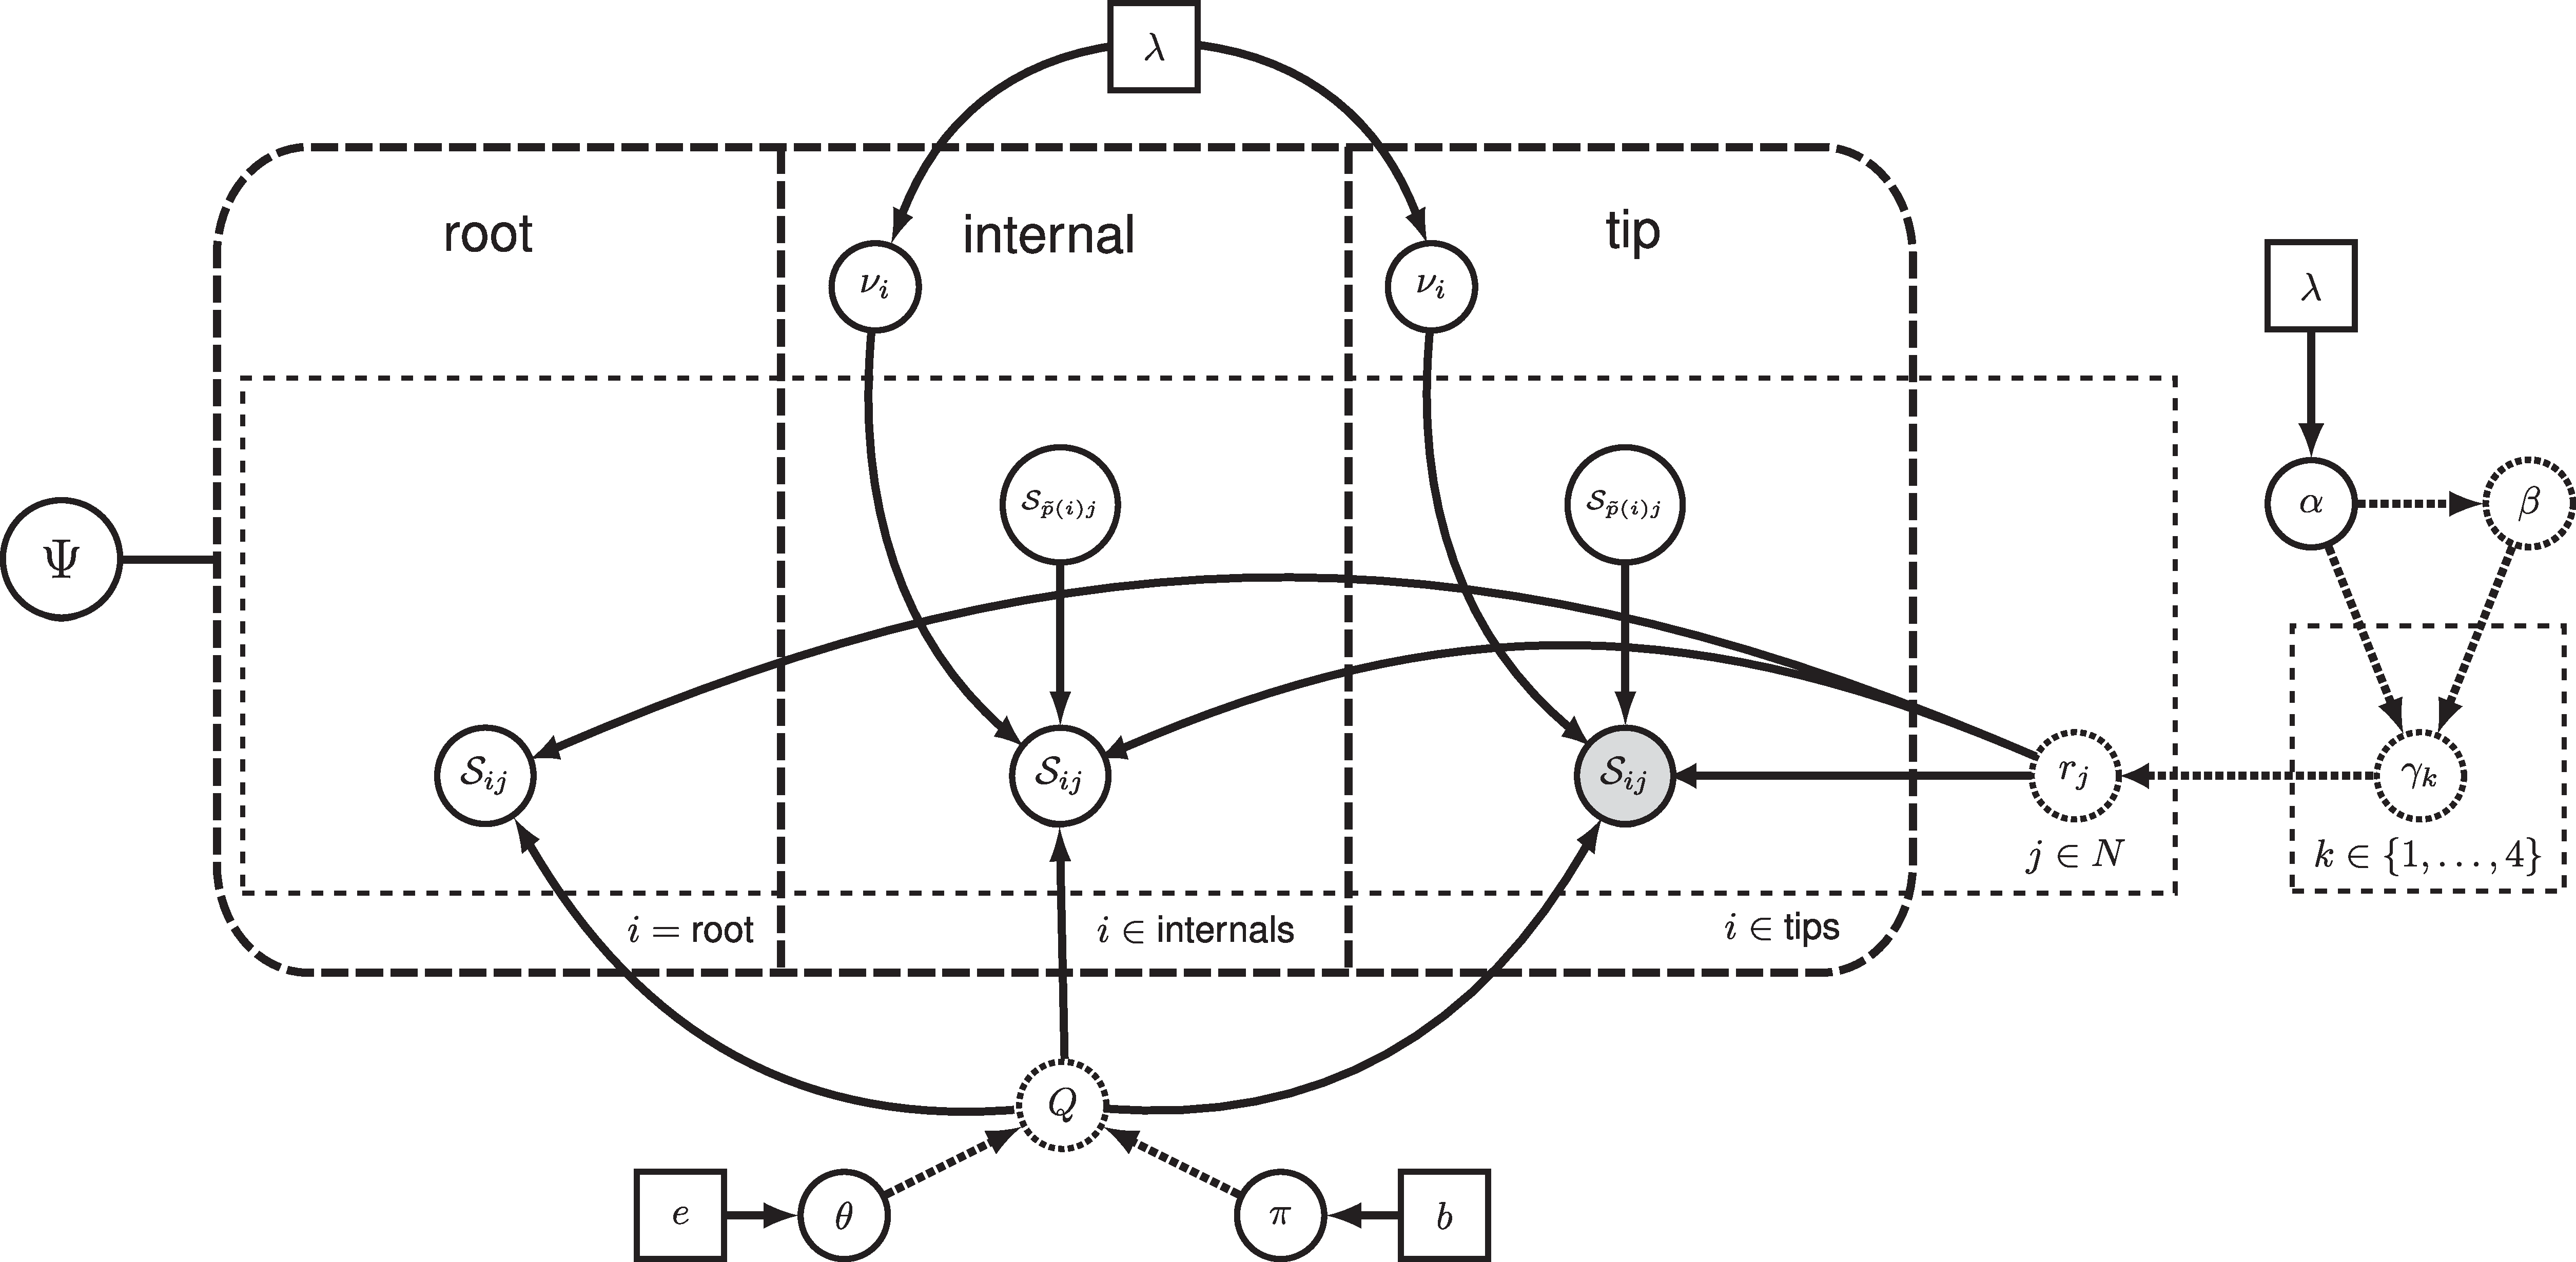
\includegraphics[width=\textwidth,angle=0]{\ResourcePath figures/gtrg_graphical_model_2.pdf}}
\caption{\small Graphical model representation of the General Time Reversible (GTR) + Gamma phylogenetic model.}
\label{fig:gtrg}
\end{figure}

\subsection{Setting up the Gamma Model in \RevBayes}

Create a constant node called \cl{shape\_prior} for the rate parameter of the exponential prior on the gamma-shape parameter (this is represented as the constant $\lambda$-rate parameter in Figure \ref{fig:gtrg}):
{\tt\begin{snugshade*}
\begin{lstlisting}
shape_prior <- 0.05                                                                             
\end{lstlisting}
\end{snugshade*}}
% I changed this from ``alpha_prior'' to match the description in the text

Then create a stochastic node called \cl{alpha} with an exponential prior (this represents the stochastic node for the $\alpha$-shape parameter in Figure \ref{fig:gtrg}):
% The GTR+G graphical model figure was not previously included...I added a modified version below that 
% horizontally compressed the GTR part of the model; the modified version is called `gtrg_graphical_model_2.'
% I changed this from \cl{shape} in tis sentence to \cl{alpha} so that it matched the description in the code and the GTR + G graphical model description
{\tt\begin{snugshade*}
\begin{lstlisting}
alpha ~ dnExponential(shape_prior)
\end{lstlisting}
\end{snugshade*}}
% I changed this from ``alpha_prior'' to match the description in the txt

The way the ASRV model is implemented involves discretizing the mean-one gamma distribution into a set number of rate categories, $k$. 
Thus, we can analytically marginalize over the uncertainty in the rate at each site. 
The likelihood of each site is averaged over the $k$ rate categories, where the rate multiplier is the mean (or median) of each of the discrete $k$ categories. 
To specify this, we need a deterministic node that is a vector that will hold the set of $k$ rates drawn from the gamma distribution with $k$ rate categories. 
The \cl{fnDiscretizeGamma()} function returns this deterministic node and takes three arguments: the shape and rate of the gamma distribution and the number of categories. 
Since we want to discretize a mean-one gamma distribution, we can pass in \cl{alpha} for both the shape and rate.
% I changed this from \cl{shape} in tis sentence to \cl{alpha} so that it matched the description in the code and the GTR + G graphical model description

Initialize the \cl{gamma\_rates} deterministic node vector using the  \cl{fnDiscretizeGamma()} function with \cl{4} bins:
{\tt \begin{snugshade*}
\begin{lstlisting}
gamma_rates := fnDiscretizeGamma( alpha, alpha, 4 )
\end{lstlisting}
\end{snugshade*}}

Note that here, by convention, we set $k = 4$.
The random variable that controls the rate variation is the stochastic node \cl{alpha}. 
% I changed this from \cl{shape} in tis sentence to \cl{alpha} so that it matched the description in the code and the GTR + G graphical model description
We will apply a simple scale move to this parameter.
{\tt \begin{snugshade*}
\begin{lstlisting}
moves[++mi] = mvScale(alpha, weight=2.0)
\end{lstlisting}
\end{snugshade*}}

Remember that you need to call the \cl{PhyloCTMC} constructor to include the new site-rate parameter:
% This sentence was incomplete previously; I think the revised version is correct.
{\tt \begin{snugshade*}
\begin{lstlisting}
seq ~ dnPhyloCTMC(tree=phylogeny, Q=Q, siteRates=gamma_rates , type="DNA")
\end{lstlisting}
\end{snugshade*}}


\subsection{Execise 4}

Modify the previous GTR analysis to specify the GTR+Gamma model. 
Run an MCMC simulation to estimate the posterior distribution.
\begin{itemize}
\item Is there an impact on the estimated phylogeny compared with the previous analyses? 
	Look at the MAP tree and the posterior probabilities of the clades.
\item What is the estimated tree length? 
	Is the estimate different to the previous analysis? What could cause this?
\item Complete the table of the phylogenetic relationship of Tarsiers.
\end{itemize}



\newpage
\section{Modeling Invariable Sites}
All of the substitution models described so far assume that the sequence data are potentially variable.
That is, we assume that the sequence data are random variables; specifically, we assume that they are realizations of the specified \cl{PhyloCTMC} distribution. 
However, some sites may not be free to vary---when the substitution rate of a site is zero, it is said to be \emph{invariable}.
Invariable sites are often confused with \emph{invariant} sites---when each species exhibits the same state, it is said to be invariant.
The concepts are related but distinct.
If a site is truly invariable, it will necessarily give rise to an invariant site pattern, as such sites will always have a zero substitution rate.
However, an invariant site pattern may be achieved via multiple substitutions that happen to end in the same state for every species.

Here we describe an extension to our phylogenetic model to accommodate invariable sites.
Under the invariable-sites model \citep[][]{Hasegawa1985}, each site is invariable with probability \cl{pinvar}, and variable with probability $1-$\cl{pinvar}.

First, let's have a look at the data and see how many invariant sites we have:
{\tt \begin{snugshade*}
\begin{lstlisting}
data.getNumInvariantSites()
\end{lstlisting}
\end{snugshade*}}
There seem to be a substantial number of invariant sites.

Now let's specify the invariable-sites model in \RevBayes.
We need to specify the prior probability that a site is invariable.
A Beta distribution is a common choice for parameters representing probabilities.
{\tt \begin{snugshade*}
\begin{lstlisting}
pinvar ~ dnBeta(1,1)
\end{lstlisting}
\end{snugshade*}}
The \cl{Beta(1,1)} distribution is a flat prior distribution that specifies equal probability for all values between 0 and 1.

Then, as usual, we add a move to change this stochastic variable; we'll used a simple sliding window move.
{\tt \begin{snugshade*}
\begin{lstlisting}
moves[mi++] = mvSlide(pinvar)
\end{lstlisting}
\end{snugshade*}}

Finally, that you need to call the \cl{PhyloCTMC} constructor to include the new\cl{pinvar} parameter:
{\tt \begin{snugshade*}
\begin{lstlisting}
seq ~ dnPhyloCTMC(tree=phylogeny, Q=Q, siteRates=gamma_rates , pInv=pinvar, type="DNA")
\end{lstlisting}
\end{snugshade*}}

\subsection{Exercise 5}

\begin{itemize}
\item Extend the GTR model to account for invariable sites and run an analysis.
\item What is the estimated probability of invariable sites and how does it relate to the ratio of invariant sites to the total number of sites?
\item Extend the GTR+$\Gamma$ model to account for invariable sites and run an analysis.
\item What is the estimated probability of invariable sites now?
\item Complete the table of the phylogenetic relationship of Tarsiers.
\end{itemize} 

\vspace{5cm}
Questions about this tutorial can be directed to: \\\vspace{-10mm}
\begin{itemize}
\item Tracy Heath (email: \href{mailto:tracyh@berkeley.edu}{tracyh@berkeley.edu}) \\\vspace{-8mm}
\item Sebastian H\"{o}hna (email: \href{mailto:sebastian.hoehna@gmail.com}{sebastian.hoehna@gmail.com}) \\\vspace{-8mm}
\item Michael Landis (email: \href{mailto:mlandis@berkeley.edu}{mlandis@berkeley.edu}) \\\vspace{-8mm} 
\item Brian R. Moore (email: \href{mailto:brianmoore@ucdavis.edu}{brianmoore@ucdavis.edu}) \\\vspace{-8mm}
\end{itemize}

\bibliographystyle{sysbio}
\bibliography{\ResourcePath refs}


\chapter{Data Partitioning}
\def \ResourcePath {RB_Partition_Tutorial/}
\section{Overview}

This tutorial provides the second protocol from our recent publication \citep{Hoehna2017a}.
The first protocol is described in the \href{https://github.com/revbayes/revbayes_tutorial/raw/master/tutorial_TeX/RB_CTMC_Tutorial/RB_CTMC_Tutorial.pdf}{Substitution model tutorial} and the third protocol is described in the \href{https://github.com/revbayes/revbayes_tutorial/raw/master/tutorial_TeX/RB_BayesFactor_Tutorial/RB_BayesFactor_Tutorial.pdf}{Bayes factor tutorial}.

This tutorial demonstrates how to accommodate variation in the substitution process across sites of an alignment.
In the preceding tutorials, we assumed that all sites in an alignment evolved under an identical substitution process.
This assumption is likely to be violated biologically, since different nucleotide sites are subject to different selection pressures, such as depending on which gene or codon position the site belongs to.
Here, we will demonstrate how to specify---and select among---alternative \emph{data partition schemes} using \RevBayes.
This is commonly referred to as partitioned-data analysis, where two or more subsets of sites in our alignment are assumed to evolve under distinct processes.

This tutorial will construct three multi-gene models.
The first model, Partition\_uniform, assumes all genes evolve under the same process parameters.
The second model, Partition\_gene, assumes all genes evolve according to the same process, but each gene has it's own set of process parameters.
The third model, Partition\_codon, partitions the data not only by gene, but also by codon position.
Each analysis will generate a \emph{maximum a posteriori} tree to summarize the inferred phylogeny.
An advanced exercise introduces how to compute Bayes factors to select across various partitioning schemes.

All of the files for this analysis are provided for you and you can run these without significant effort using the \cl{source()} function in the \RevBayes console, \EG
{\tt \begin{snugshade*}
\begin{lstlisting}
source("scripts/mcmc_Partition_uniform.Rev")
\end{lstlisting}
\end{snugshade*}}

If everything loaded properly, then you should see the program begin running the Markov chain Monte Carlo analysis needed for estimating the posterior distribution. 
If you continue to let this run, then you will see it output the states of the Markov chain once the MCMC analysis begins.

\subsection{Requirements}
We assume that you have read and hopefully completed the following tutorials:
\begin{itemize}
\item \href{https://github.com/revbayes/revbayes_tutorial/raw/master/tutorial_TeX/RB_Getting_Started/RB_Getting_Started.pdf}{Getting started}
\item \href{https://github.com/revbayes/revbayes_tutorial/raw/master/tutorial_TeX/RB_Basics_Tutorial/RB_Basics_Tutorial.pdf}{\Rev basics}
\item \href{https://github.com/revbayes/revbayes_tutorial/raw/master/tutorial_TeX/RB_CTMC_Tutorial/RB_CTMC_Tutorial.pdf}{Substitution model}
\item \href{https://github.com/revbayes/revbayes_tutorial/raw/master/tutorial_TeX/RB_BayesFactor_Tutorial/RB_BayesFactor_Tutorial.pdf}{Model selection using Bayes factors}
\end{itemize}
Note that the \href{https://github.com/revbayes/revbayes_tutorial/raw/master/tutorial_TeX/RB_Basics_Tutorial/RB_Basics_Tutorial.pdf}{\Rev basics tutorial} introduces the basic syntax of \Rev but does not cover any phylogenetic models.
You may skip the \href{https://github.com/revbayes/revbayes_tutorial/raw/master/tutorial_TeX/RB_Basics_Tutorial/RB_Basics_Tutorial.pdf}{\Rev basics tutorial} if you have some familiarity with \R.
We tried to keep this tutorial very basic and introduce all the language concepts and theory on the way.
You may only need the \href{https://github.com/revbayes/revbayes_tutorial/raw/master/tutorial_TeX/RB_Basics_Tutorial/RB_Basics_Tutorial.pdf}{\Rev basics tutorial} for a more in-depth discussion of concepts in \Rev.



%%%%%%%%
%%   Data   %%
%%%%%%%%
\section{Data and files}

We provide several data files that we will use in this tutorial; these are the same datasets that we have used in previous tutorials.
In the \cl{data} folder, you will find the following files
\begin{itemize}
\item
\cl{primates\_cytb.nex}: Alignment of the \textit{cytochrome b} subunit from 23 primates representing 14 of the 16 families (\textit{Indriidae} and \textit{Callitrichidae} are missing).
\item
\cl{primates\_cox2.nex}: Alignment of the \textit{COX-II} gene from the same 23 primates species.
\end{itemize}



\section{Introduction \& Background}

Variation in the evolutionary process across the sites of nucleotide sequence alignments is well established, and is an increasingly pervasive feature of datasets composed of gene regions sampled from multiple loci and/or different genomes.
Inference of phylogeny from these data demands that we adequately model the underlying process heterogeneity; failure to do so can lead to biased estimates of phylogeny and other parameters \citep{Brown2007}.

Accounting for process heterogeneity involves adopting a partitioned data approach (sometimes also called a `mixed-model' approach \citep{Ronquist2003}), in which the sequence alignment is first parsed into a number of data subsets that are intended to capture plausible process heterogeneity within the data.
The determination of the partitioning scheme is guided by biological considerations regarding the dataset at hand.
For example, we might wish to evaluate possible variation in the evolutionary process within a single gene region (\EG between stem and loop regions of ribosomal sequences), or among gene regions in a concatenated alignment (\EG comprising multiple nuclear loci and/or gene regions sampled from different genomes).
The choice of partitioning scheme is up to the investigator and many possible partitions might be considered for a typical dataset.

In this exercise, we assume that each data subset evolved under an independent general-time reversible model with gamma-distributed rates across sites (GTR+$\Gamma$). 
Under this model the observed data are conditionally dependent on the exchangeability rates ($\theta$), stationary base frequencies ($\pi$), and the degree of gamma-distributed among-site rate variation ($\alpha$), as well as the rooted tree ($\Psi$) and branch lengths.
We show the graphical model representation of the GTR+$\Gamma$ mode in Figure \ref{fig:pipeline}. 
When we assume different GTR+$\Gamma$ models for each data subset, this results in a composite model, in which all sites are assumed to share a common, rooted tree topology and proportional branch lengths, but subsets of sites are assumed to have independent substitution model parameters.
Finally, we perform a separate MCMC simulation to approximate the joint posterior probability density of the phylogeny and other parameters. 

For most sequence alignments, several (possibly many) partition schemes of varying complexity are plausible \emph{a priori}, which therefore requires a way to objectively identify the partition scheme that balances estimation bias and error variance associated with under- and over-parameterized mixed models, respectively.
Increasingly, partition-model selection is based on \textit{Bayes factors} \citep[\EG][]{Suchard2001}, which involves first calculating the marginal likelihood under each candidate partition scheme and then comparing the ratio of the marginal likelihoods for the set of candidate partition schemes \citep{Brandley2005,Nylander2004,Mcguire2007}.
The analysis pipeline that we will use in this tutorial is depicted in Figure \ref{fig:pipeline}.

\begin{figure}[ht!]
\centering
\fbox{\includegraphics[width=6.8in,angle=0]{\ResourcePath figures/pipeline.eps}}
\caption{\small The analysis pipeline for Exercise 1. We will explore three partition schemes for the primates dataset.
The first model (the `uniform model', $M_0$) assumes that all sites evolved under a common GTR+$\Gamma$ substitution model.
The second model (the `moderately partitioned' model, $M_1$) invokes two data subsets corresponding to the two gene regions (cytB and cox2), and assumes each subset of sites evolved under an independent GTR+$\Gamma$ model.
The final partition model (the `highly partitioned' model, $M_2$) invokes four data subsets---the first two subsets corresponds to the cytB gene region, where the first and second codon position sites are combined into one subset distinct from the third codon position sites, and the cox2 has two subsets of its own, partitioned by codon positions in the same way---and each data subset is assumed evolved under an independent GTR+$\Gamma$ substitution model.
Note that we assume that all sites share a common tree topology, $\Psi$, and branch-length proportions, for each of the candidate partition schemes.
We perform two separate sets of analyses for each partition model---a MCMC simulation to approximate the joint posterior probability density of the partition-model parameters, and a `power-posterior' MCMC simulation to approximate the marginal likelihood for each mixed model.
The resulting marginal-likelihood estimates are then evaluated using Bayes factors to assess the fit of the data to the three candidate partition models.  
}
\label{fig:pipeline}
\end{figure}
\newpage



\section{Concatenated, Non-partitioned}\label{sec:unif} 

Our first exercise is to construct a multi-gene analysis where all genes evolve under the same process and parameters.

\subsection{Setting up the model}

\subsubsection{Loading and preparing the data}

To begin, load in the sequences using the \cl{readDiscreteCharacterData()} function. 
{\tt \begin{snugshade*}
\begin{lstlisting}
data_cox2 = readDiscreteCharacterData("data/primates_cox2.nex")
data_cytb = readDiscreteCharacterData("data/primates_cytb.nex")
\end{lstlisting}
\end{snugshade*}}

Since the first step in this exercise is to assume a single model across genes, we need to combine the two datasets using {\tt concatenate()}

{\tt \begin{snugshade*}
\begin{lstlisting}
data = concatenate( data_cox2, data_cytb )
\end{lstlisting}
\end{snugshade*}}

Typing \cl{data} reports the dimensions of the concatenated matrix, this provides information about the alignment:


{\tt \begin{snugshade*}
\begin{lstlisting}

   DNA character matrix with 23 taxa and 1852 characters
   =====================================================
   Origination:                   primates_cox2.nex
   Number of taxa:                23
   Number of included taxa:       23
   Number of characters:          1852
   Number of included characters: 1852
   Datatype:                      DNA

\end{lstlisting}
\end{snugshade*}}

For later use, we will store the taxon information (\cl{taxa}) and the number of taxa and branches.
{\tt \begin{snugshade*}
\begin{lstlisting}
n_species <- data.ntaxa()
n_branches <- 2 * n_species - 3
taxa <- data.taxa()
\end{lstlisting}
\end{snugshade*}}

Additionally, we will create some move and monitor index variables to create our move and monitor vectors.
{\tt \begin{snugshade*}
\begin{lstlisting}
mvi = 0
mni = 0
\end{lstlisting}
\end{snugshade*}}

\subsubsection{Substitution model}

Now we can proceed with building our GTR$+\Gamma$ model.
First, we will define and specify a prior on the exchangeability rates of the GTR model

{\tt \begin{snugshade*}
\begin{lstlisting}
er_prior <- v(1,1,1,1,1,1) 
er ~ dnDirichlet( er_prior )
\end{lstlisting}
\end{snugshade*}}

and assign its moves

{\tt \begin{snugshade*}
\begin{lstlisting}
moves[++mvi] = mvBetaSimplex(er, alpha=10, tune=true, weight=3) 
moves[++mvi] = mvDirichletSimplex(er, alpha=10.0, tune=true, weight=1.0)
\end{lstlisting}
\end{snugshade*}}

We can use the same type of distribution as a prior on the 4 stationary frequencies ($\pi_A, \pi_C, \pi_G, \pi_T$) since these parameters also represent proportions. 
Specify a flat Dirichlet prior density on the base frequencies:
{\tt \begin{snugshade*}
\begin{lstlisting}
pi_prior <- v(1,1,1,1) 
pi ~ dnDirichlet( pi_prior )
\end{lstlisting}
\end{snugshade*}}

The node \cl{pi} represents the $\pi$ node in Figure \ref{pipeline}.
Now add the simplex scale move on the stationary frequencies to the moves vector

{\tt \small \begin{snugshade*}
\begin{lstlisting}
moves[++mvi] = mvBetaSimplex(pi, alpha=10, tune=true, weight=2) 
moves[++mvi] = mvDirichletSimplex(pi, alpha=10.0, tune=true, weight=1.0)
\end{lstlisting}
\end{snugshade*}}

We can finish setting up this part of the model by creating a deterministic node for the GTR rate matrix \cl{Q}. 
The \cl{fnGTR()} function takes a set of exchangeability rates and a set of base frequencies to compute the rate matrix used when calculating the likelihood of our model.
{\tt \begin{snugshade*}
\begin{lstlisting}
Q := fnGTR(er,pi)
\end{lstlisting}
\end{snugshade*}}


\subsubsection{Among site rate variation}

We will also assume that the substitution rates vary among sites according to an one-parametric gamma distribution, \IE where the shape equals the rate ($\alpha=\beta$) and thus with mean 1.0 \citep{Yang1994a}. 
Since we do not have good prior knowledge about the variance in site rates, thus we can place a relative diffuse lognormal prior on the shape parameter.
Create a constant node called \cl{alpha\_prior\_mean} for the mean parameter and a constant node called \cl{alpha\_prior\_sd} for the standard deviation of the lognormal prior on the gamma-shape parameter (this is represented as the constant $m_\alpha$ and $sd_\alpha$ parameters in Figure \ref{fig:gtrg}):
{\tt\begin{snugshade*}
\begin{lstlisting}
alpha_prior_mean <- ln(2.0)
alpha_prior_sd <- 0.587405
\end{lstlisting}
\end{snugshade*}}

Then create a stochastic node called \cl{alpha} with a lognormal prior:
{\tt\begin{snugshade*}
\begin{lstlisting}
alpha ~ dnLognormal( alpha_prior_mean, alpha_prior_sd )
\end{lstlisting}
\end{snugshade*}}

The way the ASRV model is implemented involves discretizing the mean-one gamma distribution into a set number of rate categories. 
Thus, we can analytically marginalize over the uncertainty in the rate at each site. 
To do this, we need a deterministic node that is a vector of rates calculated from the gamma distribution and the number of rate categories. 
The \cl{fnDiscretizeGamma()} function returns this deterministic node and takes three arguments: the shape and rate of the gamma distribution and the number of categories. 
Since we want to discretize a mean-one gamma distribution, we can pass in \cl{alpha} for both the shape and rate.

Initialize the \cl{gamma\_rates} deterministic node vector using the  \cl{fnDiscretizeGamma()} function with \cl{4} bins:
{\tt \begin{snugshade*}
\begin{lstlisting}
gamma_rates := fnDiscretizeGamma( alpha, alpha, 4, false )
\end{lstlisting}
\end{snugshade*}}

The random variable that controls the rate variation is the stochastic node \cl{alpha}. 
This variable is a single, real positive value (\cl{RevType = RealPos}). 
We will apply a simple scale move to this parameter.
The scale move's tuning parameter is called \cl{lambda} and this value dictates the size of the proposal.
{\tt \begin{snugshade*}
\begin{lstlisting}
moves[++mvi] = mvScale(alpha, lambda=0.1, tune=false, weight=4.0)
\end{lstlisting}
\end{snugshade*}}

\subsubsection{Invariant sites}

Invariant sites (sites that remain fixed throughout their evolutionary history) may be seen as an extreme case of among-site rate variation.
In contrast to $+ \Gamma$ models, the $+I$ model allows site some probability of having substitution rate equal to zero.
Here, we give the probability of a site being invariant with \cl{pinvar}
{\tt \begin{snugshade*}
\begin{lstlisting}
pinvar ~ dnBeta(1,1)
moves[++mvi] = mvScale(pinvar, lambda=0.1, tune=false, weight=2.0)
moves[++mvi] = mvSlide(pinvar, delta=10.0, tune=false, weight=2.0)
\end{lstlisting}
\end{snugshade*}}



\subsubsection{Tree prior}

The tree topology and branch lengths are also stochastic nodes in our model. 
In Figure \ref{pipeline}, the tree topology is denoted $\Psi$ and the length of the branch leading to node $i$ is $\nu_i$.

For simplicity, we will use the same prior distribution on the tree topology, a uniform topology prior, and branch lengths, independent exponential prior distributions, as done in the \href{https://github.com/revbayes/revbayes_tutorial/raw/master/tutorial_TeX/RB_CTMC_Tutorial/RB_CTMC_Tutorial.pdf}{substitution model tutorial}.

We will assume that all possible labeled, unrooted tree topologies have equal probability. 
This is the \cl{dnUniformTopology()} distribution in \RevBayes. 
Note that in \RevBayes it is advisable to specify the outgroup for your study system if you use an unrooted tree prior, whereas other software, \EG \MrBayes uses the first taxon in the data matrix file as the outgroup.
Specify the \cl{topology} stochastic node by passing in the tip labels \cl{names} to the \cl{dnUniformTopology()} distribution:
{\tt \begin{snugshade*}
\begin{lstlisting}
out_group = clade("Galeopterus_variegatus")
topology ~ dnUniformTopology(taxa, outgroup=out_group)
\end{lstlisting}
\end{snugshade*}}

To update the unrooted tree topology, we can use both a nearest-neighbor interchange move (\cl{mvNNI}) and a subtree-prune and regrafting move (\cl{mvSPR}). 
These moves do not have tuning parameters associated with them, thus you only need to pass in the \cl{topology} node and proposal \cl{weight}. 
{\tt \begin{snugshade*}
\begin{lstlisting}
moves[++mvi] = mvNNI(topology, weight=1.0)
moves[++mvi] = mvSPR(topology, weight=1.0)
\end{lstlisting}
\end{snugshade*}}
The weight specifies how often the move will be applied either on average per iteration or relative to all other moves.
Have a look at the \href{https://github.com/revbayes/revbayes_tutorial/raw/master/tutorial_TeX/RB_MCMC_Tutorial/RB_MCMC_Tutorial.pdf}{MCMC Diagnosis tutorial} for more details about moves and MCMC strategies (found on the \href{http://revbayes.github.io/tutorials.html}{\RevBayes~Tutorials Website}).


Next we have to create a stochastic node for each of the $2N-3$ branches in our tree (where $N=$ \cl{n\_species}). 
We can do this using a \cl{for} loop --- this is a plate in our graphical model. In this loop, we can create each of the branch-length nodes and assign each move. 
Copy this entire block of \Rev~code into the console:
{\tt \small \begin{snugshade*}
\begin{lstlisting}
for (i in 1:n_branches) {
   br_lens[i] ~ dnExponential(10.0)
   moves[++mvi] = mvScale(br_lens[i]) 
}
\end{lstlisting}
\end{snugshade*}}

It is convenient for monitoring purposes to add the tree length as deterministic variable. 
The tree length is simply the sum of all branch lengths. .
Accordingly, the tree length can be computed using the \cl{sum()} function, which calculates the sum of any vector of values.
{\tt \begin{snugshade*}
\begin{lstlisting}
TL := sum(br_lens)
\end{lstlisting}
\end{snugshade*}}


Finally, we can create a \emph{phylogram} (a phylogeny in which the branch lengths are proportional to the expected number of substitutions/site) by combining the tree topology and branch lengths.
We do this using the \cl{treeAssembly()} function, which applies the value of the $i^{th}$ member of the \cl{br\_lens} vector to the branch leading to the $i^{th}$ node in \cl{topology}. 
Thus, the \cl{phylogeny} variable is a deterministic node: 
{\tt \begin{snugshade*}
\begin{lstlisting}
phylogeny := treeAssembly(topology, br_lens)
\end{lstlisting}
\end{snugshade*}}

\impmark{Fore more information on tree priors please read the \href{https://github.com/revbayes/revbayes_tutorial/raw/master/tutorial_TeX/RB_DiversificationRate_Tutorial/RB_DiversificationRate_Tutorial.pdf}{RB\_DiversificationRate\_Tutorial}.}


\subsection{Putting it All Together}

We now have all the parameters needed to model the phylogenetic molecular substitution process

{\tt \begin{snugshade*}
\begin{lstlisting}
phyloSeq ~ dnPhyloCTMC(tree=psi, Q=Q,  siteRates=gamma_rates, pInv=pinvar, type="DNA")
\end{lstlisting}
\end{snugshade*}}

To compute the likelihood, we condition the process on the data observed at the tips of the tree

{\tt \begin{snugshade*}
\begin{lstlisting}
phyloSeq.clamp(data)
\end{lstlisting}
\end{snugshade*}}

Since the model is now specified, we wrap the components in a {\tt Model} object.

{\tt \begin{snugshade*}
\begin{lstlisting}
mymodel = model(Q)
\end{lstlisting}
\end{snugshade*}}


\subsubsection{Specifying Monitors}

For our MCMC analysis we need to set up a vector of \textit{monitors} to save the states of our Markov chain. 
The monitor functions are all called \cl{mn*}, where \cl{*} is the wildcard representing the monitor type.
First, we will initialize the model monitor using the \cl{mnModel} function. This creates a new monitor variable that will output the states for all model parameters when passed into a MCMC function. 
{\tt \begin{snugshade*}
\begin{lstlisting}
monitors[++mni] = mnModel(filename="output/PS_uniform.log",printgen=10)
\end{lstlisting}
\end{snugshade*}}

The \cl{mnFile} monitor will record the states for only the parameters passed in as arguments. We use this monitor to specify the output for our sampled trees and branch lengths.

{\tt \begin{snugshade*}
\begin{lstlisting}
monitors[++mni] = mnFile(psi, filename="output/PS_uniform.trees", printgen=10)
\end{lstlisting}
\end{snugshade*}}

Finally, create a screen monitor that will report the states of specified variables to the screen with \cl{mnScreen}:
{\tt \begin{snugshade*}
\begin{lstlisting}
monitors[++mni] = mnScreen(alpha, pinvar, TL, printgen=1000)
\end{lstlisting}
\end{snugshade*}}


\subsubsection{Initializing and Running the MCMC Simulation}

With a fully specified model, a set of monitors, and a set of moves, we can now set up the MCMC algorithm that will sample parameter values in proportion to their posterior probability. The \cl{mcmc()} function will create our MCMC object:
{\tt \begin{snugshade*}
\begin{lstlisting}
mymcmc = mcmc(mymodel, monitors, moves, nruns=2)
\end{lstlisting}
\end{snugshade*}}
Note that this will automatically run two independent replicated MCMC simulations because we specified \cl{nruns=2}.

We can run the \cl{.burnin()} member function if we wish to pre-run the chain and discard the initial states. 
{\tt \begin{snugshade*}
\begin{lstlisting}
mymcmc.burnin(generations=10000,tuningInterval=100)
\end{lstlisting}
\end{snugshade*}}


Now, run the MCMC:
{\tt \begin{snugshade*}
\begin{lstlisting}
mymcmc.run(generations=30000)
\end{lstlisting}
\end{snugshade*}}

When the analysis is complete, you will have the monitor files in your output directory.

\RevBayes~can also summarize the tree samples by reading in the tree-trace file:
{\tt \begin{snugshade*}
\begin{lstlisting}
treetrace = readTreeTrace("output/PS_uniform.trees", treetype="non-clock")
treetrace.summarize()
\end{lstlisting}
\end{snugshade*}}


The \cl{mapTree()} function will summarize the tree samples and write the maximum a posteriori tree to file:
{\tt \begin{snugshade*}
\begin{lstlisting}
map_tree = mapTree(treetrace,"output/PS_uniform_map.tre")
\end{lstlisting}
\end{snugshade*}}

This completes the uniform partition analysis.
The next two sections will implement more complex partitioning schemes in a similar manner.


\section{Partitioning by Gene Region}\label{secByGene}

The uniform model used in the previous section assumes that all sites in the alignment evolved under the same process described by a shared tree, branch length proportions, and parameters of the GTR+$\Gamma$ substitution model.
However, our alignment contains two distinct gene regions---cytB and cox2---so we may wish to explore the possibility that the substitution process differs between these two gene regions.
This requires that we first specify the data partitions corresponding to these two genes, then define an independent substitution model for each data partition. 

First, we'll clear the workspace of all declared variables
{\tt \begin{snugshade*}
\begin{lstlisting}
clear()
\end{lstlisting}
\end{snugshade*}}

Since we wish to avoid individually specifying each parameter of the GTR+$\Gamma$ model for each of our data partitions, we can \textit{loop} over our datasets and create vectors of nodes.
To do this, we begin by creating a vector of data file names:
{\tt \begin{snugshade*}
\begin{lstlisting}
filenames <- v("data/primates_cox2.nex", "data/primates_cytb.nex")
\end{lstlisting}
\end{snugshade*}}

Set a variable for the number of partitions:
{\tt \begin{snugshade*}
\begin{lstlisting}
n_data_subsets <- filenames.size()
\end{lstlisting}
\end{snugshade*}}

And create a vector of data matrices called \cl{data}:
{\tt \begin{snugshade*}
\begin{lstlisting}
for (i in 1:n_data_subsets){
   data[i] = readDiscreteCharacterData(filenames[i])
}
\end{lstlisting}
\end{snugshade*}}

Next, we can initialize some important variables. This does require, however, that both of our alignments have the same number of species and matching tip names.
{\tt \begin{snugshade*}
\begin{lstlisting}
taxa <- data[1].taxa()
\end{lstlisting}
\end{snugshade*}}

{\tt \begin{snugshade*}
\begin{lstlisting}
mvi = 0 
mni = 0
\end{lstlisting}
\end{snugshade*}}


\subsection{Specify the Parameters by Looping Over Partitions}

We can avoid creating unique names for every node in our model if we use a \cl{for} loop to iterate over our partitions. Thus, we will only have to type in our entire GTR+$\Gamma$ model parameters once. 
This will produce a vector for each of the unlinked parameters ---\EG there will be a vector of \cl{alpha} nodes where the stochastic node for the first partition (cytB) will be \cl{alpha[1]} and the stochastic node for the second partition (cox2) will be called \cl{alpha[2]}.

The script for the model, {\tt RevBayes\_scripts/mcmc\_Partition\_gene.Rev}, creates the model parameters for each partition in one large loop.
Here, we will split the loop into smaller parts to achieve the same end.

First, we will create the GTR rate matrix for partition $i$ by first creating exchangeability rates
{\tt \small \begin{snugshade*}
\begin{lstlisting}
for (i in 1:n_data_subsets) {
  er_prior[i] <- v(1,1,1,1,1,1)
  er[i] ~ dnDirichlet(er_prior[i])
  moves[++mvi] = mvBetaSimplex(er[i], alpha=10, tune=true, weight=3) 
}
\end{lstlisting}
\end{snugshade*}}

and stationary frequencies

{\tt \small \begin{snugshade*}
\begin{lstlisting}
for (i in 1:n_data_subsets) {
  pi_prior[i] <- v(1,1,1,1)
  pi[i] ~ dnDirichlet(pi_prior[i])
  moves[++mvi] = mvBetaSimplex(pi[i], alpha=10, tune=true, weight=2)
}
\end{lstlisting}
\end{snugshade*}}

then passing those parameters into a rate matrix function

{\tt \small \begin{snugshade*}
\begin{lstlisting}
for (i in 1:n_data_subsets) {
  Q[i] := fnGTR(er[i],pi[i]) 
}
\end{lstlisting}
\end{snugshade*}}

which states the rate matrix ({\tt Q[i]}) for partition $i$ is determined by the exchangeability rates ({\tt er[i]}) and stationary frequencies ({\tt pi[i]}) also defined for partition $i$.
Following this format, we construct the remaining partition parameters: the $+\Gamma$ mixture model

{\tt \small \begin{snugshade*}
\begin{lstlisting}
for (i in 1:n_data_subsets) {
    alpha_prior_mean[i] <- ln(2.0)
    alpha_prior_sd[i] <- 0.587405
    alpha[i] ~ dnLognormal( alpha_prior_mean[i], alpha_prior_sd[i] )
    gamma_rates[i] := fnDiscretizeGamma( alpha[i], alpha[i], 4, false )

    moves[++mvi] = mvScale(alpha[i],weight=2)
}
\end{lstlisting}
\end{snugshade*}}

the $+I$ invariant sites model

{\tt \small \begin{snugshade*}
\begin{lstlisting}
for (i in 1:n_data_subsets) {
  pinvar[i] ~ dnBeta(1,1)
  moves[++mvi] = mvScale(pinvar[i], lambda=0.1, tune=true, weight=2.0)
  moves[++mvi] = mvSlide(pinvar[i], delta=0.1, tune=true, weight=2.0)
}
\end{lstlisting}
\end{snugshade*}}

and the per-partition substitution rate multipliers 
{\tt \small \begin{snugshade*}
\begin{lstlisting}
# specify a rate multiplier for each partition
part_rate_mult ~ dnDirichlet( rep(1.0, n_data_subsets) )
moves[++mvi] = mvBetaSimplex(part_rate_mult, alpha=1.0, tune=true, weight=n_data_subsets)
moves[++mvi] = mvDirichletSimplex(part_rate_mult, alpha=1.0, tune=true, weight=2.0)

# note that we use here a vector multiplication, 
# i.e., multiplying each element of part_rate_mult by n_data_subsets
part_rate := part_rate_mult * n_data_subsets\end{lstlisting}
\end{snugshade*}}


\begin{framed}
\textbf{Different Substitution Models for each Gene}\\
Alternatively, we might be interested in applying different substitution models for each gene independently instead of assuming the same substitution albeit with different parameters for each gene.
In this two gene case this is rather simple to do by specifying the substitution model for each gene independently.
For many genes this might become lengthy and you might want to write a script to generate this section (note: we may provide such scripts soon).

For simplicity and sake of demonstration, we assume that the cytochrome b region evolves under a Jukes-Cantor substitution model and the COX-II gene under an HKY substitution model.
We begin with the cytochrome b gene and the Jukes-Cantor substitution model:
{\tt \small \begin{snugshade*}
\begin{lstlisting}
# specify the JC rate matrix
Q[1] <- fnJC(4)
\end{lstlisting}
\end{snugshade*}}

Second, we specify the HKY substitution model for the COX-II gene:
{\tt \begin{snugshade*}
\begin{lstlisting}
pi_prior <- v(1,1,1,1) 
pi ~ dnDirichlet(pi_prior)

# specify a move to propose updates to on pi
moves[++mvi] = mvBetaSimplex(pi, weight=2)
moves[++mvi] = mvDirichletSimplex(pi, weight=1)

# specify a lognormal distribution as the prior distribution on kappa
kappa ~ dnLognormal(0.0,1.25)

# a simple scaling move to update kappa
moves[++mvi] = mvScale(kappa)

# Finally, create the HKY rate matrix
Q[2] := fnHKY(kappa,pi)
\end{lstlisting}
\end{snugshade*}}
Note that we specified manually in this way our vector of rate matrices \cl{Q}.
We can thus specify any substitution model manually for a given gene.
We hope that this brief example conveys the idea how to specify gene-specific substitution models.
You can add rate-variation among sites and/or probabilities for a site being invariant for each gene too.
Finally, you can then either loop over all genes to create the \cl{dnPhyloCTMC} distribution (see below) if the structure of the model allows it (\IE if all models have a variable for site-rate-variation and probabilities for invariant site), or you efficiently set these variables to default values (\EG \cl{pinvar[i]=0.0} if there is no probability for a site being invariant for this gene), or you create the \cl{seq[i] $\sim$ dnPhyloCTMC(...)} manually outside a loop as well. 
\end{framed}


\subsubsection{Tree prior}

We assume that both genes evolve along the same tree.
Hence, we need to specify a random variable for our tree parameter which is the same as was specified for {\tt mcmc\_Partition\_uniform.Rev}.
{\tt \begin{snugshade*}
\begin{lstlisting}
out_group = clade("Galeopterus_variegatus")
# Prior distribution on the tree topology	
topology ~ dnUniformTopology(taxa, outgroup=out_group)
moves[++mvi] = mvNNI(topology, weight=5.0)
moves[++mvi] = mvSPR(topology, weight=1.0)

# Branch length prior
for (i in 1:n_branches) {
    bl[i] ~ dnExponential(10.0)
	moves[++mvi] = mvScale(bl[i])
}

TL := sum(bl)
	
psi := treeAssembly(topology, bl)
\end{lstlisting}
\end{snugshade*}}


\subsection{Putting it all together}

Since we have a rate matrix and a site-rate model for each partition, we must create a phylogenetic CTMC for each gene. 
Additionally, we must fix the values of these nodes by attaching their respective data matrices.
These two nodes are linked by the \cl{psi} node and their log-likelihoods are added to get the likelihood of the whole DAG.
{\tt \begin{snugshade*}
\begin{lstlisting}
for (i in 1:n_data_subsets) {
  phyloSeq[i] ~ dnPhyloCTMC(tree=psi, Q=Q[i], branchRates=part_rate_mult[i], siteRates=norm_gamma_rates[i], pInv=pinvar[i], type="DNA")
  phyloSeq[i].clamp(data[i])
}
\end{lstlisting}
\end{snugshade*}}

The remaining steps should be familiar:
wrap the model components in a model object

{\tt \begin{snugshade*}
\begin{lstlisting}
mymodel = model(psi)
\end{lstlisting}
\end{snugshade*}}

\subsection{Create monitors}

create the monitors

{\tt \begin{snugshade*}
\begin{lstlisting}
monitors[++mni] = mnModel(filename="output/PS_gene.log",printgen=10)
monitors[++mni] = mnFile(psi, filename="output/PS_gene.trees", printgen=100)
monitors[++mni] = mnScreen(TL, printgen=1000)
\end{lstlisting}
\end{snugshade*}}

configure and run the MCMC analysis

{\tt \begin{snugshade*}
\begin{lstlisting}
mymcmc = mcmc(mymodel, moves, monitors, nruns=2)
mymcmc.burnin(10000,100)
mymcmc.run(30000)
\end{lstlisting}
\end{snugshade*}}

and summarize the posterior density of trees with a MAP tree

{\tt \begin{snugshade*}
\begin{lstlisting}
treetrace = readTreeTrace("output/PS_gene.trees", treetype="non-clock")
treetrace.summarize()
mapTree(treetrace,"output/PS_gene_MAP.tre")
\end{lstlisting}
\end{snugshade*}}



\section{Partitioning by Codon Position and by Gene}\label{secExtremeP}

Because of the genetic code, we often find that different positions within a codon (first, second, and third) evolve at different rates.
Thus, using our knowledge of biological data, we can devise a third approach that further partitions our alignment. 
For this exercise, we will partition sites within the cytB and cox2 gene by codon position.

{\tt \begin{snugshade*}
\begin{lstlisting}
clear()
data_cox2 <- readDiscreteCharacterData("data/primates_cox2.nex")
data_cytb <- readDiscreteCharacterData("data/primates_cytb.nex")
\end{lstlisting}
\end{snugshade*}}

We must now add our codon-partitions to the \cl{data} vector.
The first and second elements in the {\tt data} vector will describe cytB data, and the third and fourth elements will describe cox2 data.
Moreover, the first and third elements will describe the evolutionary process for the first and second codon position sites, while the second and fourth elements describe the process for the third codon position sites alone.

We can create this by calling the helper function \cl{setCodonPartition()}, which is a member function of the data matrix. 
We are assuming that the gene is \textit{in frame}, meaning the first column in your alignment is a first codon position. 
The \cl{setCodonPartition()} function takes a single argument, the position of the alignment you wish to extract. 
It then returns every third column, starting at the index provided as an argument.

Before we can use the use the \cl{setCodonPartition()} function, we must first populate the position in the \cl{data} matrix with some sequences. 
Then we call the member function of \cl{data[1]} to exclude all but the 1$^{st}$ and 2$^{nd}$ positions for cox2.
{\tt \begin{snugshade*}
\begin{lstlisting}
data[1] <- data_cox2
data[1].setCodonPartition( v(1,2) )
\end{lstlisting}
\end{snugshade*}}

Assign the 3$^{rd}$ codon positions for cox2 to \cl{data[2]}:
{\tt \begin{snugshade*}
\begin{lstlisting}
data[2] <- data_cox2
data[2].setCodonPartition( 3 )
\end{lstlisting}
\end{snugshade*}}

Then repeat for cytB, being careful to store the subsetted data to elements 3 and 4:
{\tt \begin{snugshade*}
\begin{lstlisting}
data[3] <- data_cytb
data[3].setCodonPartition( v(1,2) )
data[4] <- data_cytb
data[4].setCodonPartition( 3 )
\end{lstlisting}
\end{snugshade*}}

Now we have a data vector containing for subset.
We can then specify the independent substitution models per data subset.
The remaining parts of the model are identical to the previous exercise where we partitioned by gene.

\impmark{Don't forget to rename the output files!}

\subsection{Exercises}
\begin{enumerate}

\item {\bf Reviewing posterior estimates.} Open the {\tt PS\_codon.log} file in \Tracer. Remember that data subsets 1 and 2 are for cox2, partitions 3 and 4 are for cytB, subsets 1 and 3 are for sites in the first and second codon positions (per gene), and subsets 2 and 4 are for sites in the third and fourth codon positions (per gene).

Aside from the tree topology and branch lengths, each data subset is modeled to have its own set of parameters.
However, the posterior estimates for some parameters appear quite similar between some pairs of subsets yet different between other pairs of subsets.
For example, {\tt part\_rate} is the per-subset substitution rate.
This clock is approximately one order of magnitude faster for partitions 2 and 4 (third codon position sites) than it is for subsets 1 and 3 (non-third codon position sites).

Identify other parameter-subset relationships like this in the posterior.
Under this model, would you consider the gene or the codon site position to hold greater influence over the site's evolutionary mode?

\item {\bf Comparison of MAP trees.} Open the three inferred MAP trees in \FigTree.
Check to enable ``Node Labels'', click ``Display'' and select ``posterior'' from the dropdown menu.
Internal nodes now report the probability of the clade appearing in the posterior density of sampled trees.
Do different models yield different tree topologies?
Generally, do complex models provide higher or lower clade support?

\item {\bf Partitioned model selection.}
Bayes factors are computed as the ratio of marginal likelihoods (see the \href{https://github.com/revbayes/revbayes_tutorial/raw/master/tutorial_TeX/RB_BayesFactor_Tutorial/RB_BayesFactor_Tutorial.pdf}{model selection using Bayes factors tutorial} for more details).
Rather than constructing the analysis with an {\tt mcmc} object, marginal likelihood computations rely on output from a {\tt powerPosterior} object.

Copy {\tt mcmc\_Partition\_uniform.Rev} to {\tt ml\_Partition\_uniform.Rev}.
In {\tt ml\_Partition\_uniform.Rev}, delete all lines after the {\tt model} function is called, so the MCMC is never run and the MAP tree is never computed.

Instead, configure and run a power posterior analysis

{\tt \begin{snugshade*}
\begin{lstlisting}
pow_p = powerPosterior(mymodel, moves, monitors, "output/model_uniform.out", cats=100)
pow_p.burnin(generations=5000,tuningInterval=200)
pow_p.run(generations=2000)
\end{lstlisting}
\end{snugshade*}}

then compute the marginal likelihood using the stepping stone sampler

{\tt \begin{snugshade*}
\begin{lstlisting}
ss = steppingStoneSampler(file="output/model_uniform.out", powerColumnName="power", likelihoodColumnName="likelihood")
ss.marginal()
\end{lstlisting}
\end{snugshade*}}

and again using the path sampler

{\tt \begin{snugshade*}
\begin{lstlisting}
ps = pathSampler(file="model_uniform.out", powerColumnName="power", likelihoodColumnName="likelihood")
ps.marginal()\end{lstlisting}
\end{snugshade*}}


%\item {\bf 4) Customized partition models (advanced).} Create the partitioned model where first, second, and third codon positions are partitioned per gene.
%The substitution parameters for each partition are independent {\it except} the first and second codon positions per gene share stationary frequencies.
%These parameters would be $\pi_{12}^{(cytB)}$, $\pi_{3}^{(cytB)}$, $\pi_{12}^{(cox2)}$, $\pi_{3}^{(cox2)}$.
%
%The easiest way to accomplish this is to copy {\tt model\_PS2.Rev} to {\tt model\_PS3.Rev} and modify the new file's contents.
%Specifically, you will need to adjust how the codon position partitions are defined to yield six (instead of four) partitions.
%When looping over partitions, you will need an if-statement to assign stationary frequencies properly.
%Take some care when applying monitors and moves to the new model.


\end{enumerate}


\bibliographystyle{sysbio}
\bibliography{\GlobalResourcePath refs}




\part{Inference}

\chapter{Markov chain Monte Carlo Algorithms}
\include{RB_MCMC_Tutorial/RB_MCMC_Tutorial_content}

\chapter{Model Selection and Bayes Factors}
\def \ResourcePath {RB_BayesFactor_Tutorial/}
\section{Overview}


This tutorial demonstrates how to set up and perform an analysis that computes the marginal likelihood of a given model.
We will show how to calculates Bayes factors to select among different substitution model and different partition configurations of aligned DNA sequences. 

\subsection{Requirements}
We assume that you have read and hopefully completed the following tutorials:
\begin{itemize}
\item RB\_Getting\_Started
\item RB\_Data\_Tutorial
\item RB\_CTMC\_Tutorial
\end{itemize}
This means, we expect that you are able to start \RevBayes, know some basic commands, how to load data into \RevBayes~and run a single gene phylogenetic analysis (assuming an unconstrained/unrooted tree).



%%%%%%%%
%%   Data   %%
%%%%%%%%
\section{Data and files}

We provide several data files which we will use in this tutorial.
You may want to use your own data instead.
In the \cl{data} folder, you will find the following files
\begin{itemize}
\item
\cl{primates_cytb.nex}: Alignment of the \textit{cytochrome b} subunit from 23 primates representing 14 of the 16 families (\textit{Indriidae} and \textit{Callitrichidae} are missing).
\item
\cl{primates_16s.nex}: Alignment of the \textit{16s ribosomal RNA} gene from the same 23 primates species.
\item
\cl{primates_cox2.nex}: Alignment of the \textit{COX-2} gene from the same 23 primates species.
\end{itemize}



\section{Introduction}

For most sequence alignments, several (possibly many) substitution models and partition schemes of varying complexity are plausible {\it a priori}, which therefore requires a way to objectively identify the model that balances estimation bias and error variance associated with under- and over-parameterized models, respectively.
Increasingly, model selection is based on \textit{Bayes factors} \citep[{\it e.g.},][]{Suchard2001,Lartillot2006,Xie2011,Baele2012,Baele2013}, which involves first calculating the marginal likelihood under each candidate model and then comparing the ratio of the marginal likelihoods for the set of candidate model.

 
Given two models, $M_0$ and $M_1$, the Bayes factor comparison assessing the relative plausibility of each model as an explanation of the data, $BF(M_0,M_1)$, is:
$$BF(M_0,M_1) = \frac{\mbox{posterior odds}}{\mbox{prior odds}}.$$
The posterior odds is the posterior probability of $M_0$ given the data, $\mathbf X$, divided by the posterior odds of $M_1$ given the data:
$$\mbox{posterior odds} = \frac{\mathbb{P}(M_0 \mid \mathbf X)}{\mathbb{P}(M_1 \mid \mathbf X)},$$
and the prior odds is the prior probability of $M_0$ divided by the prior probability of $M_1$:
$$\mbox{prior odds} = \frac{\mathbb{P}(M_0)}{\mathbb{P}(M_1)}.$$
Thus, the Bayes factor measures the degree to which the data alter our belief regarding the support for $M_0$ relative to $M_1$ \citep{Lavine1999}:
\begin{align}\label{BFeq1}
BF(M_0,M_1) = \frac{\mathbb{P}(M_0 \mid \mathbf X, \theta_0)}{\mathbb{P}(M_1 \mid \mathbf X, \theta_1)} \div \frac{\mathbb{P}(M_0)}{\mathbb{P}(M_1)}. 
\end{align}
This, somewhat vague, definition does not lead to clear-cut identification of the ``best'' model. Instead, \textsl{you} must decide the degree of your belief in $M_0$ relative to $M_1$. 
Despite the absence of any strict ``rule-of-thumb'', you can refer to the scale \citep[outlined by][]{Jeffreys1961} for interpreting these measures (Table \ref{bftable}).
\begin{table}[h]
\centering
\caption{\small The scale for interpreting Bayes factors by Harold \citet{Jeffreys1961}.} 
\label{bftable}
\begin{tabular}{l c c c}
\hline
\multicolumn{1}{r}{{Strength of evidence}} & \multicolumn{1}{l}{\textbf{$BF(M_0, M_1)$}} & \multicolumn{1}{l}{\textbf{log($BF(M_0, M_1)$)}} &  \multicolumn{1}{l}{\textbf{$\text{log}_{10}$($BF(M_0, M_1)$)}}\\ 
\hline
Negative (supports $M_1$) & $<1$ & $<0$ & $<0$\\
Barely worth mentioning & $1$ to $3.2$ & $0$ to $1.16$ & $0$ to $0.5$\\
Substantial & $3.2$ to $10$ & $1.16$ to $2.3$ & $0.5$ to $1$ \\
Strong & $10$ to $100$ & $2.3$ to $4.6$ & $1$ to $2$ \\
Decisive& $>100$ & $>4.6$ & $>2$ \\
\hline
\multicolumn{3}{l}{{\scriptsize{For a detailed description of Bayes factors see \citet{Kass1995}}}} 
\end{tabular}
\end{table}


Unfortunately, direct calculation of the posterior odds to prior odds ratio is unfeasible for most phylogenetic models. However, we can further define the posterior odds ratio as:
\begin{align*}
\frac{\mathbb{P}(M_0 \mid \mathbf X)}{\mathbb{P}(M_1 \mid \mathbf X)} = \frac{\mathbb{P}(M_0)}{\mathbb{P}(M_1)} \frac{\mathbb{P}(\mathbf X \mid M_0)}{\mathbb{P}(\mathbf X \mid M_1)},
\end{align*}
where $\mathbb{P}(\mathbf X \mid M_i)$ is the \textit{marginal likelihood} of the data marginalized over all parameters for $M_i$; it is also referred to as the \textit{model evidence} or \textit{integrated likelihood}.
More explicitly, the marginal likelihood is the probability of the set of observed data ($\mathbf X$) under a given model ($M_i$), while averaging over all possible values of the parameters of the model ($\theta_i$) with respect to the prior density on $\theta_i$
\begin{align}\label{margeLike}
\mathbb{P}(\mathbf X \mid M_i) = \int \mathbb{P}(\mathbf X \mid \theta_i) \mathbb{P}(\theta_i)dt.
\end{align}
If you refer back to equation \ref{BFeq1}, you can see that, with very little algebra, the ratio of marginal likelihoods is equal to the Bayes factor:
\begin{align}\label{bfFormula}
BF(M_0,M_1) = \frac{\mathbb{P}(\mathbf X \mid M_0)}{\mathbb{P}(\mathbf X \mid M_1)} = \frac{\mathbb{P}(M_0 \mid \mathbf X, \theta_0)}{\mathbb{P}(M_1 \mid \mathbf X, \theta_1)} \div \frac{\mathbb{P}(M_0)}{\mathbb{P}(M_1)}. 
\end{align}
Therefore, we can perform a Bayes factor comparison of two models by calculating the marginal likelihood for each one. % Simple as pie, right?
Alas, exact solutions for calculating marginal likelihoods are not known for phylogenetic models (see equation \ref{margeLike}), thus we must resort to numerical integration methods to estimate or approximate these values. 
In this exercise, we will estimate the marginal likelihood for each partition scheme
using both the stepping-stone \citep{Xie2011,Fan2011} and path sampling estimators \citep{Lartillot2006, Baele2012}. 



\bigskip
\subsection{Phylogenetic Models}\label{secUnif} 

The models we use here are equivalent to the models described in the previous exercise on substitution models (continuous time Markov models).
To specify the model please consult the previous exercise. Specifically, you need to specify a 
\begin{itemize}
\item Jukes-Cantor substitution model
\item Hasegawa-Kishino-Yano substitution model
\item General-Time-Reversible substitution model
\item Gamma distributed rate variation among sites
\item Invariant sites model
\end{itemize}


\bigskip
\subsection{Estimating the Marginal Likelihood}

With a fully specified model, we can set up the \cl{powerPosterior()} analysis to create a file of `powers' and likelihoods from which we can estimate the marginal likelihood using stepping-stone or path sampling. 
This method computes a vector of powers from a beta distribution, then executes an MCMC run for each power step while raising the likelihood to that power. In this implementation, the vector of powers starts with 1, sampling the likelihood close to the posterior and incrementally sampling closer and closer to the prior as the power decreases. 



%\textbf{\textit{Clear Workspace and Load the Data and Model}}

Just to be safe, it is better to clear the workspace (if you did not just restart \RevBayes)
{\tt \begin{snugshade*}
\begin{lstlisting}
clear()
\end{lstlisting}
\end{snugshade*}}

Now set up the model as in the previous exercise. You should start with the simple Jukes-Cantor substitution model. Setting up the model will involve
\begin{enumerate}
\item Loading the data and retrieving useful variables about the data (\EG number of sequences and taxon names).
\item Specify the rate matrix of the substitution model.
\item Specify the tree model including branch length variables.
\item Create a random variable for the sequences that evolved under the \cl{PhyloCTMC}.
\item Clamp the data.
\item Create a model object.
\item Don't forget the moves!
\end{enumerate}

The following description of how-to specify a marginal likelihood computation is valid for any model in \RevBayes.
You need to repeat this later for other models.
First, we create the variable containing the power posterior analysis. 
This requires us to provide a model and vector of moves, as well as an output file name. 
The \cl{cats} argument sets the number of power steps.
{\tt \begin{snugshade*}
\begin{lstlisting}
pow_p = powerPosterior(mymodel, moves, "model1.out", cats=50) 
\end{lstlisting}
\end{snugshade*}}

We can start the power posterior analysis by first burning in the chain and and discarding the first 10000 states.  
This will help the analysis to start from the posterior distribution instead of any random parameter state.
{\tt \begin{snugshade*}
\begin{lstlisting}
pow_p.burnin(generations=10000,tuningInterval=1000)
\end{lstlisting}
\end{snugshade*}}

Now execute the run with the \cl{.run()} function:
{\tt \begin{snugshade*}
\begin{lstlisting}
pow_p.run(generations=1000)  
\end{lstlisting}
\end{snugshade*}}

Once the power posteriors have been saved to file, create a stepping stone sampler. 
This function can read any file of power posteriors and compute the marginal likelihood using stepping-stone sampling. 
{\tt \small \begin{snugshade*}
\begin{lstlisting}
ss <- steppingStoneSampler(file="model1.out", powerColumnName="power", likelihoodColumnName="likelihood")
\end{lstlisting}
\end{snugshade*}}

Compute the marginal likelihood under stepping-stone sampling using the member function \cl{marginal()} of the \cl{ss} variable and record the value in Table \ref{ssTable}.
{\tt \begin{snugshade*}
\begin{lstlisting}
ss.marginal() 
\end{lstlisting}
\end{snugshade*}}

Path sampling is an alternative to stepping-stone sampling and also takes the same power posteriors as input. 
{\tt \small \begin{snugshade*}
\begin{lstlisting}
ps = pathSampler(file="model1.out", powerColumnName="power", likelihoodColumnName="likelihood")
\end{lstlisting}
\end{snugshade*}}

Compute the marginal likelihood under stepping-stone sampling using the member function \cl{marginal()} of the \cl{ps} variable and record the value in Table \ref{ssTable}.
{\tt \begin{snugshade*}
\begin{lstlisting}
ps.marginal() 
\end{lstlisting}
\end{snugshade*}}

\noindent \\ \impmark As an example we provide the file \textbf{RevBayes\_scripts/marginalLikelihood\_JukesCantor.Rev}.


\subsection{Exercises}

\begin{itemize}
\item Compute the marginal likelihoods of the \textit{cytb} alignment for the following substitution models
\begin{itemize}
\item Jukes-Cantor substitution model
\item Hasegawa-Kishino-Yano substitution model
\item General-Time-Reversible substitution model
\item General-Time-Reversible substitution model with gamma distributed rate variation among sites
\item General-Time-Reversible substitution model with invariant sites
\item General-Time-Reversible substitution model with gamma distributed rate variation among sites and the invariant sites model
\end{itemize}
\item Fill the marginal likelihood estimates in Table~\ref{tab:ml_cytb}.
\item Repeat the marginal likelihood computation for the \textit{MT-ND1 gene} and fill Table~\ref{tab:ml_nd1}.
\item Which is the best fitting substitution model?
\end{itemize}

\begin{Form}
\begin{table}[h]
\centering
\caption{\small Estimated marginal likelihoods for different substitution models for the cytb alignment$^*$.}
\begin{tabular}{l c c c c}
\hline
\multicolumn{1}{l}{\textbf{ }} &\multicolumn{1}{r}{\textbf{ }} & \multicolumn{3}{c}{\textbf{Marginal lnL estimates}} \\ 
\cline{3-5}
\multicolumn{1}{l}{\textbf{Substitution Model}} & \multicolumn{1}{r}{\hspace{3mm}} & \multicolumn{1}{c}{\textit{Stepping-stone}} & \multicolumn{1}{r}{\hspace{3mm}} & \multicolumn{1}{c}{\textit{Path sampling}} \\ 
\hline
JC ($M_1$) & \hspace{15mm} & \TextField[name=gene1_m11,backgroundcolor={.85 .85 .85},color={1 0 0},height=4ex]{}  & \hspace{15mm} & \TextField[name=gene1_m12,backgroundcolor={.85 .85 .85},color={0 0 1},height=4ex]{} \\
\hline
HKY ($M_2$) & \hspace{3mm} &\TextField[name=gene1_m21,backgroundcolor={.85 .85 .85},color={1 0 0},height=4ex]{}   & \hspace{3mm} & \TextField[name=gene1_m22,backgroundcolor={.85 .85 .85},color={0 0 1},height=4ex]{} \\
\hline
GTR ($M_3$) & \hspace{3mm} &\TextField[name=gene1_m31,backgroundcolor={.85 .85 .85},color={1 0 0},height=4ex]{}   & \hspace{3mm} & \TextField[name=gene1_m32,backgroundcolor={.85 .85 .85},color={0 0 1},height=4ex]{} \\
\hline
GTR+$\Gamma$ ($M_4$) & \hspace{3mm} & \TextField[name=gene1_m41,backgroundcolor={.85 .85 .85},color={1 0 0},height=4ex]{} & \hspace{3mm} & \TextField[name=gene1_m42,backgroundcolor={.85 .85 .85},color={0 0 1},height=4ex]{} \\
\hline
GTR+I ($M_5$) & \hspace{3mm} & \TextField[name=gene1_m51,backgroundcolor={.85 .85 .85},color={1 0 0},height=4ex]{} & \hspace{3mm} & \TextField[name=gene1_m52,backgroundcolor={.85 .85 .85},color={0 0 1},height=4ex]{} \\
\hline
GTR+$\Gamma$+I ($M_6$) & \hspace{3mm} & \TextField[name=gene1_m61,backgroundcolor={.85 .85 .85},color={1 0 0},height=4ex]{} & \hspace{3mm} & \TextField[name=gene1_m62,backgroundcolor={.85 .85 .85},color={0 0 1},height=4ex]{} \\
\hline
Any other model ($M_7$) & \hspace{3mm} & \TextField[name=gene1_m71,backgroundcolor={.85 .85 .85},color={1 0 0},height=4ex]{} & \hspace{3mm} & \TextField[name=gene1_m72,backgroundcolor={.85 .85 .85},color={0 0 1},height=4ex]{} \\
\hline
Any other model ($M_8$) & \hspace{3mm} & \TextField[name=gene1_m81,backgroundcolor={.85 .85 .85},color={1 0 0},height=4ex]{} & \hspace{3mm} & \TextField[name=gene1_m82,backgroundcolor={.85 .85 .85},color={0 0 1},height=4ex]{} \\
\hline
Any other model ($M_9$) & \hspace{3mm} & \TextField[name=gene1_m91,backgroundcolor={.85 .85 .85},color={1 0 0},height=4ex]{} & \hspace{3mm} & \TextField[name=gene1_m92,backgroundcolor={.85 .85 .85},color={0 0 1},height=4ex]{} \\
\hline
{\footnotesize{$^*$you can edit this table}}\\
\end{tabular}
\label{tab:ml_cytb}
\end{table}
\end{Form}


\begin{Form}
\begin{table}[h]
\centering
\caption{\small Estimated marginal likelihoods for different substitution models of the ND1 gene$^*$.}
\begin{tabular}{l c c c c}
\hline
\multicolumn{1}{l}{\textbf{ }} &\multicolumn{1}{r}{\textbf{ }} & \multicolumn{3}{c}{\textbf{Marginal lnL estimates}} \\ 
\cline{3-5}
\multicolumn{1}{l}{\textbf{Substitution Model}} & \multicolumn{1}{r}{\hspace{3mm}} & \multicolumn{1}{c}{\textit{Stepping-stone}} & \multicolumn{1}{r}{\hspace{3mm}} & \multicolumn{1}{c}{\textit{Path sampling}} \\ 
\hline
JC ($M_1$) & \hspace{15mm} & \TextField[name=gene2_m11,backgroundcolor={.85 .85 .85},color={1 0 0},height=4ex]{}  & \hspace{15mm} & \TextField[name=gene2_m12,backgroundcolor={.85 .85 .85},color={0 0 1},height=4ex]{} \\
\hline
HKY ($M_2$) & \hspace{3mm} &\TextField[name=gene2_m21,backgroundcolor={.85 .85 .85},color={1 0 0},height=4ex]{}   & \hspace{3mm} & \TextField[name=gene2_m22,backgroundcolor={.85 .85 .85},color={0 0 1},height=4ex]{} \\
\hline
GTR ($M_3$) & \hspace{3mm} &\TextField[name=gene2_m31,backgroundcolor={.85 .85 .85},color={1 0 0},height=4ex]{}   & \hspace{3mm} & \TextField[name=gene2_m32,backgroundcolor={.85 .85 .85},color={0 0 1},height=4ex]{} \\
\hline
GTR+$\Gamma$ ($M_4$) & \hspace{3mm} & \TextField[name=gene2_m41,backgroundcolor={.85 .85 .85},color={1 0 0},height=4ex]{} & \hspace{3mm} & \TextField[name=gene2_m42,backgroundcolor={.85 .85 .85},color={0 0 1},height=4ex]{} \\
\hline
GTR+I ($M_5$) & \hspace{3mm} & \TextField[name=gene2_m51,backgroundcolor={.85 .85 .85},color={1 0 0},height=4ex]{} & \hspace{3mm} & \TextField[name=gene2_m52,backgroundcolor={.85 .85 .85},color={0 0 1},height=4ex]{} \\
\hline
GTR+$\Gamma$+I ($M_6$) & \hspace{3mm} & \TextField[name=gene2_m61,backgroundcolor={.85 .85 .85},color={1 0 0},height=4ex]{} & \hspace{3mm} & \TextField[name=gene2_m62,backgroundcolor={.85 .85 .85},color={0 0 1},height=4ex]{} \\
\hline
Any other model ($M_7$) & \hspace{3mm} & \TextField[name=gene2_m71,backgroundcolor={.85 .85 .85},color={1 0 0},height=4ex]{} & \hspace{3mm} & \TextField[name=gene2_m72,backgroundcolor={.85 .85 .85},color={0 0 1},height=4ex]{} \\
\hline
Any other model ($M_8$) & \hspace{3mm} & \TextField[name=gene2_m81,backgroundcolor={.85 .85 .85},color={1 0 0},height=4ex]{} & \hspace{3mm} & \TextField[name=gene2_m82,backgroundcolor={.85 .85 .85},color={0 0 1},height=4ex]{} \\
\hline
Any other model ($M_9$) & \hspace{3mm} & \TextField[name=gene2_m91,backgroundcolor={.85 .85 .85},color={1 0 0},height=4ex]{} & \hspace{3mm} & \TextField[name=gene2_m92,backgroundcolor={.85 .85 .85},color={0 0 1},height=4ex]{} \\
\hline
{\footnotesize{$^*$you can edit this table}}\\
\end{tabular}
\label{tab:ml_nd1}
\end{table}
\end{Form}





\FloatBarrier
\section{Compute Bayes Factors and Select Model}


Now that we have estimates of the marginal likelihood under each of our different models, we can evaluate their relative plausibility using Bayes factors.
Phylogenetics software programs log-transform the likelihood to avoid \href{http://en.wikipedia.org/wiki/Arithmetic_underflow}{underflow}, because multiplying likelihoods results in numbers that are too small to be held in computer memory.
Thus, we must use a different form of equation \ref{bfFormula} to calculate the ln-Bayes factor (we will denote this value $\mathcal{K}$):
\begin{align}\label{LNbfFormula}
\mathcal{K}=\ln[BF(M_0,M_1)] = \ln[\mathbb{P}(\mathbf X \mid M_0)]-\ln[\mathbb{P}(\mathbf X \mid M_1)],
\end{align}
where $\ln[\mathbb{P}(\mathbf X \mid M_0)]$ is the \textit{marginal lnL} estimate for model $M_0$. 
The value resulting from equation \ref{LNbfFormula} can be converted to a raw Bayes factor by simply taking the exponent of $\cal{K}$
\begin{align}\label{LNbfFormula2}
BF(M_0,M_1) = e^{\cal{K}}.
\end{align}
Alternatively, you can interpret the strength of evidence in favor of $M_0$ using the $\cal{K}$ and skip equation \ref{LNbfFormula2}. 
In this case, we evaluate the $\cal{K}$ in favor of model $M_0$ against model $M_1$ so that:
\begin{center}
\begin{tabular}{l}
if $\mathcal{K} > 1$, then model $M_0$ wins\\
if $\mathcal{K} < -1$, then model $M_1$ wins.
\end{tabular}
\end{center}
Thus, values of $\mathcal{K}$ around 0 indicate ambiguous support. 

Using the values you entered in Table \ref{tab:ml_cytb} and equation \ref{LNbfFormula},  calculate the ln-Bayes factors (using $\mathcal{K}$) for the different model comparisons. 
Enter your answers in Table \ref{bfTable} using the stepping-stone and the path-sampling estimates of the marginal log likelihoods. 

\begin{Form}
\begin{table}[h!]
\centering
\caption{\small Bayes factor calculation$^*$.}
\resizebox{\textwidth}{!}{%  
\begin{tabular}{l c c c c c c c c c}
\hline
\textbf{Model comparison} & $M_1$ & $M_2$ & $M_3$ & $M_4$ & $M_5$ & $M_6$ & $M_7$ & $M_8$ & $M_9$ \\ 
\hline
$M_1$ & - & \TextField[name=bf12,backgroundcolor={.85 .85 .85},color={0 0 1},height=4ex]{}  & \TextField[name=bf13,backgroundcolor={.85 .85 .85},color={0 0 1},height=4ex]{}  & \TextField[name=bf14,backgroundcolor={.85 .85 .85},color={0 0 1},height=4ex]{}  & \TextField[name=bf15,backgroundcolor={.85 .85 .85},color={0 0 1},height=4ex]{}  & \TextField[name=bf16,backgroundcolor={.85 .85 .85},color={0 0 1},height=4ex]{}  & \TextField[name=bf17,backgroundcolor={.85 .85 .85},color={0 0 1},height=4ex]{}  & \TextField[name=bf18,backgroundcolor={.85 .85 .85},color={0 0 1},height=4ex]{}  & \TextField[name=bf19,backgroundcolor={.85 .85 .85},color={0 0 1},height=4ex]{} \\
\hline
$M_2$ & \TextField[name=bf21,backgroundcolor={.85 .85 .85},color={1 0 0},height=4ex]{}  & - & \TextField[name=bf23,backgroundcolor={.85 .85 .85},color={0 0 1},height=4ex]{}  & \TextField[name=bf24,backgroundcolor={.85 .85 .85},color={0 0 1},height=4ex]{}  & \TextField[name=bf25,backgroundcolor={.85 .85 .85},color={0 0 1},height=4ex]{}  & \TextField[name=bf26,backgroundcolor={.85 .85 .85},color={0 0 1},height=4ex]{}  & \TextField[name=bf27,backgroundcolor={.85 .85 .85},color={0 0 1},height=4ex]{}  & \TextField[name=bf28,backgroundcolor={.85 .85 .85},color={0 0 1},height=4ex]{}  & \TextField[name=bf29,backgroundcolor={.85 .85 .85},color={0 0 1},height=4ex]{} \\
\hline
$M_3$ & \TextField[name=bf31,backgroundcolor={.85 .85 .85},color={1 0 0},height=4ex]{}  & \TextField[name=bf32,backgroundcolor={.85 .85 .85},color={0 0 1},height=4ex]{}  & -  & \TextField[name=bf34,backgroundcolor={.85 .85 .85},color={0 0 1},height=4ex]{}  & \TextField[name=bf35,backgroundcolor={.85 .85 .85},color={0 0 1},height=4ex]{}  & \TextField[name=bf36,backgroundcolor={.85 .85 .85},color={0 0 1},height=4ex]{}  & \TextField[name=bf37,backgroundcolor={.85 .85 .85},color={0 0 1},height=4ex]{}  & \TextField[name=bf38,backgroundcolor={.85 .85 .85},color={0 0 1},height=4ex]{}  & \TextField[name=bf39,backgroundcolor={.85 .85 .85},color={0 0 1},height=4ex]{} \\
\hline
$M_4$ & \TextField[name=bf41,backgroundcolor={.85 .85 .85},color={1 0 0},height=4ex]{}  & \TextField[name=bf42,backgroundcolor={.85 .85 .85},color={0 0 1},height=4ex]{}  & \TextField[name=bf43,backgroundcolor={.85 .85 .85},color={0 0 1},height=4ex]{}  &-  & \TextField[name=bf45,backgroundcolor={.85 .85 .85},color={0 0 1},height=4ex]{}  & \TextField[name=bf46,backgroundcolor={.85 .85 .85},color={0 0 1},height=4ex]{}  & \TextField[name=bf47,backgroundcolor={.85 .85 .85},color={0 0 1},height=4ex]{}  & \TextField[name=bf48,backgroundcolor={.85 .85 .85},color={0 0 1},height=4ex]{}  & \TextField[name=bf49,backgroundcolor={.85 .85 .85},color={0 0 1},height=4ex]{} \\
\hline
$M_5$ & \TextField[name=bf51,backgroundcolor={.85 .85 .85},color={1 0 0},height=4ex]{}  & \TextField[name=bf52,backgroundcolor={.85 .85 .85},color={0 0 1},height=4ex]{}  & \TextField[name=bf53,backgroundcolor={.85 .85 .85},color={0 0 1},height=4ex]{}  & \TextField[name=bf54,backgroundcolor={.85 .85 .85},color={0 0 1},height=4ex]{}  & -  & \TextField[name=bf56,backgroundcolor={.85 .85 .85},color={0 0 1},height=4ex]{}  & \TextField[name=bf57,backgroundcolor={.85 .85 .85},color={0 0 1},height=4ex]{}  & \TextField[name=bf58,backgroundcolor={.85 .85 .85},color={0 0 1},height=4ex]{}  & \TextField[name=bf59,backgroundcolor={.85 .85 .85},color={0 0 1},height=4ex]{} \\
\hline
$M_6$ & \TextField[name=bf61,backgroundcolor={.85 .85 .85},color={1 0 0},height=4ex]{}  & \TextField[name=bf62,backgroundcolor={.85 .85 .85},color={0 0 1},height=4ex]{}  & \TextField[name=bf63,backgroundcolor={.85 .85 .85},color={0 0 1},height=4ex]{}  & \TextField[name=bf64,backgroundcolor={.85 .85 .85},color={0 0 1},height=4ex]{}  & \TextField[name=bf65,backgroundcolor={.85 .85 .85},color={0 0 1},height=4ex]{}  & - & \TextField[name=bf67,backgroundcolor={.85 .85 .85},color={0 0 1},height=4ex]{}  & \TextField[name=bf68,backgroundcolor={.85 .85 .85},color={0 0 1},height=4ex]{}  & \TextField[name=bf69,backgroundcolor={.85 .85 .85},color={0 0 1},height=4ex]{} \\
\hline
$M_7$ & \TextField[name=bf71,backgroundcolor={.85 .85 .85},color={1 0 0},height=4ex]{}  & \TextField[name=bf72,backgroundcolor={.85 .85 .85},color={0 0 1},height=4ex]{}  & \TextField[name=bf73,backgroundcolor={.85 .85 .85},color={0 0 1},height=4ex]{}  & \TextField[name=bf74,backgroundcolor={.85 .85 .85},color={0 0 1},height=4ex]{}  & \TextField[name=bf75,backgroundcolor={.85 .85 .85},color={0 0 1},height=4ex]{}  & \TextField[name=bf76,backgroundcolor={.85 .85 .85},color={0 0 1},height=4ex]{}  &-  & \TextField[name=bf78,backgroundcolor={.85 .85 .85},color={0 0 1},height=4ex]{}  & \TextField[name=bf79,backgroundcolor={.85 .85 .85},color={0 0 1},height=4ex]{} \\
\hline
$M_8$ & \TextField[name=bf81,backgroundcolor={.85 .85 .85},color={1 0 0},height=4ex]{}  & \TextField[name=bf82,backgroundcolor={.85 .85 .85},color={0 0 1},height=4ex]{}  & \TextField[name=bf83,backgroundcolor={.85 .85 .85},color={0 0 1},height=4ex]{}  & \TextField[name=bf84,backgroundcolor={.85 .85 .85},color={0 0 1},height=4ex]{}  & \TextField[name=bf85,backgroundcolor={.85 .85 .85},color={0 0 1},height=4ex]{}  & \TextField[name=bf86,backgroundcolor={.85 .85 .85},color={0 0 1},height=4ex]{}  & \TextField[name=bf87,backgroundcolor={.85 .85 .85},color={0 0 1},height=4ex]{}  & - & \TextField[name=bf89,backgroundcolor={.85 .85 .85},color={0 0 1},height=4ex]{} \\
\hline
$M_9$ & \TextField[name=bf91,backgroundcolor={.85 .85 .85},color={1 0 0},height=4ex]{}  & \TextField[name=bf92,backgroundcolor={.85 .85 .85},color={0 0 1},height=4ex]{}  & \TextField[name=bf93,backgroundcolor={.85 .85 .85},color={0 0 1},height=4ex]{}  & \TextField[name=bf94,backgroundcolor={.85 .85 .85},color={0 0 1},height=4ex]{}  & \TextField[name=bf95,backgroundcolor={.85 .85 .85},color={0 0 1},height=4ex]{}  & \TextField[name=bf96,backgroundcolor={.85 .85 .85},color={0 0 1},height=4ex]{}  & \TextField[name=bf97,backgroundcolor={.85 .85 .85},color={0 0 1},height=4ex]{}  & \TextField[name=bf98,backgroundcolor={.85 .85 .85},color={0 0 1},height=4ex]{}  & - \\
\hline
{\footnotesize{$^*$you can edit this table}}\\
\end{tabular}}
\label{bfTable}
\end{table}
\end{Form}



\newpage
\section{Partitioned Analysis}
Now that you have identified the best substitution model for each of the two genes, we will run a joint analysis under both genes: a partitioned analysis.




\vspace{5cm}
Questions about this tutorial can be directed to: \\\vspace{-10mm}
\begin{itemize}
\item Tracy Heath (email: \href{mailto:tracyh@berkeley.edu}{tracyh@berkeley.edu}) \\\vspace{-8mm}
\item Michael Landis (email: \href{mailto:mlandis@berkeley.edu}{mlandis@berkeley.edu}) \\\vspace{-8mm} 
\item Sebastian H\"{o}hna (email: \href{mailto:sebastian.hoehna@gmail.com}{sebastian.hoehna@gmail.com})
\end{itemize}


\bibliographystyle{sysbio}
\bibliography{\ResourcePath refs}





\part{Dating}
\chapter{Dating and Relaxed Clocks}
\def \ResourcePath {RB_RelaxedClock_Tutorial/}
\include{RB_RelaxedClock_Tutorial/RB_RelaxedClock_Tutorial_content}


\part{Diversification Rate Estimation}
\chapter{Simple Diversification Rate Estimation}
\def \ResourcePath {RB_SimpleDiversification_Tutorial/}
\include{RB_SimpleDiversification_Tutorial/RB_SimpleDiversification_Tutorial_content}


\part{Gene tree - Species tree estimation}
\chapter{Gene tree - Species tree estimation}
\def \ResourcePath {RB_GTST_Tutorial/}
\input{\ResourcePath RB_GTST_Tutorial_content_no_bib}



\bibliographystyle{sysbio}
\bibliography{\GlobalResourcePath refs}




\part{Biogeography}
\chapter{Many Area DEC}
\def \ResourcePath {RB_Biogeography_Tutorial/}
\include{RB_Biogeography_Tutorial/RB_Biogeography_Tutorial_content}


\part{Phylogenetic Comparative Method}
\chapter{Phylogenetic Comparative Analyses: Continuous Trait Evolution}
\def \ResourcePath {RB_PhyloComparative_Tutorial/}
\section{Introduction}

The subject of the comparative method is the analysis of trait evolution at the macroevolutionary scale.
In a comparative context, many different questions can be addressed: tempo and mode of evolution, correlated evolution of multiple quantitative traits, trends and bursts, changes in evolutionary mode correlated with major key innovations in some groups, etc \citep[for a good introduction see][]{Harvey1991}.

In order to correctly formalize comparative questions, the underlying phylogeny should always be explicitly accounted for. This point is clearly illustrated, in particular, by the independent contrasts method \citep{Felsenstein1985,Huelsenbeck2003}. Practically speaking, the phylogeny and the divergence times are usually first estimated using a separate phylogenetic reconstruction software. In a second step, this time-calibrated phylogeny is used as an input to the comparative method.
Doing this, however, raises a certain number of methodological problems:
\begin{itemize}
\item
the uncertainty about the phylogeny (and about divergence times) is ignored
\item
the traits themselves may have something to say about the phylogeny
\item
the rate of substitution, and more generally the parameters of the substitution process, can also be seen as quantitative traits, amenable to a comparative analysis.
\end{itemize}
All these points are not easily formalized in the context of the step-wise approach mentioned above.
Instead, what all this suggests is that phylogenetic reconstruction, molecular dating and the comparative method should all be considered jointly, in the context of one single overarching probabilistic model.

Thanks to its modular structure, \RevBayes~represents a natural framework for attempting this integration.
The aim of the present tutorial is to guide you through a series of examples where this integration is achieved, step by step.
It can also be considered as an example of the more general perspective of \emph{integrative modeling}, which can be recruited in many other contexts.



%%%%%%%%
%%   Data   %%
%%%%%%%%
\section{Data and files}

We provide several data files which we will use in this tutorial.
You may want to use your own data instead.
In the \cl{data} folder, you will find the following files
\begin{itemize}
\item
\cl{primates\_cytb.nex}: Alignment of the \textit{cytochrome b} subunit from 23 primates representing 14 of the 16 families (\textit{Indriidae} and \textit{Callitrichidae} are missing).

\item
\cl{primates\_lhtlog.nex}: 2 life-history traits (endocranial volume (ECV), body mass; each for males and females separately)  for 23 primate species \citep[taken from the Anage database,][]{DeMagalhaes2009}. The traits have been log-transformed.

\item
\cl{primates.tree}: A time calibrated phylogeny of the same 23 primates.
\end{itemize}





\section{Univariate Brownian evolution of quantitative traits}

\label{univariate}

As a first preliminary exercise, we wish to reconstruct the evolution of body mass in primates and, in particular, estimate the body mass of their last common ancestor.
For this, we will assume that the logarithm of body mass follows a simple univariate Brownian motion along the phylogeny.
In a first step, we will ignore phylogenetic uncertainty:
thus, we will assume that the Brownian process describing body mass evolution runs along a fixed time-calibrated phylogeny (with fixed divergence times), such as specified in the file \cl{primates.tree}.

\noindent \\ \impmark You may want to take the time to visualize the tree given in \cl{primates.tree} as well as the matrix of quantitative traits specified by the \cl{primates\_lhtlog.nex} file, before going into the modeling work described below.


\subsection{The model and the priors}

A univariate Brownian motion $x(t)$ is parameterized by its starting value at the root of the phylogeny $x(0)$ and a rate parameter $\sigma$. This rate parameter tunes the amplitude of the variation per unit of time. Specifically, along a given time interval $(0,T)$, the value of $X$ at time $T$ is normally distributed, with mean $x(0)$ and variance $\sigma^2 T$:
\begin{eqnarray*}
x(T) & \sim & \text{Normal} \left( x(0), \sigma^2 T \right).
\end{eqnarray*}

Concerning $\sigma$, we can formalize the idea that we are ignorant about the \emph{scale} (the order of magnitude) of this parameter by using a log-uniform prior:
\begin{eqnarray*}
\sigma &\sim& \frac{1}{\sigma}.
\end{eqnarray*}

Concerning the initial value $x(0)$ of the Brownian process at the root of the phylogeny.
Alternatively, you may want to specify a normal distribution as the prior distribution on the root value if you have some prior information.

Finally, the tree topology $\psi$ is, as mentioned above, fixed to some externally given phylogeny.
The entire model is now specified: tree $\psi$, variance $\sigma$ and Brownian process $x(t)$:
\begin{eqnarray*}
\sigma &\sim& \frac{1}{\sigma},
\\
x(0) &\sim& \text{Uniform},
\\
x(t) \mid \Psi, \sigma &\sim& \text{Brownian} \left( x(0), \, \psi, \, \sigma \right).
\end{eqnarray*}
Conditioning the model on empirical data by clamping $x(t)$ at the tips of the phylogeny, we can then run a MCMC to sample from the joint posterior distribution on $\sigma$ and $x$. Once this is done, we can obtain posterior means, medians or credible intervals for the value of body mass or other life-history traits for specific ancestors.


\subsection{Programming the model in \RevBayes}

The problem of continuous trait evolution ---just as for discrete trait evolution--- along a phylogeny is that we do not know the values of the traits at the internal nodes. That means, that we need to treat the states at the internal nodes as additional parameters of the model. For discrete characters we use the sum-product (a.k.a.~pruning) algorithm \citep{Felsenstein1981} to analytically integrate over all possible states at the internal nodes. For continuous characters (traits) similar methods have been proposed.
In \RevBayes~you have three main ways of specifying this model and running an analysis on it. The three approaches are: (1) phylogenetic independent contrasts using the reduced likelihood (REML), (2) Brownian motion using a phylogenetic covariance matrix, and (3) a full Brownian motion model using data augmentation.
Each of these approaches has there advantages and disadvantages as will be explained below.
Nevertheless, all approaches give the same results in terms of rate estimation.


\subsection{Phylogenetic Independent Contrasts using the reduced likelihood (REML)}

The reduced or restricted maximum likelihood (REML) method computes the probability of observing the continuous character at the tips by an analytical solution to integrate over the internal states \citep{Felsenstein1985}. 
This analytical solution is very fast to compute and thus can be applied to large phylogenies and/or many independent characters. However, the REML method looses the information about the location of the root state and thus you cannot infer which state the root or other internal nodes have.

You do not need to understand the algorithm but we provide a sketch of the idea behind REML to give you some insights.
REML compute the values at the internal nodes as the phylogenetic contrasts $x_k = x_i - x_j$ where $x_i$ and $x_j$ are the values of the child nodes in the phylogeny.
Then, we can compute the probability of observing the contrast $x_k$ using the probability density of a normal distribution with mean $\mu = 0$ and standard deviation $\sigma = \sqrt{\nu_i + \delta_i + \nu_j + \delta_j}$ where $\nu_i$ and $\nu_j$ are the (scaled) branch lengths leading to node $i$ and $j$ respectively. $\delta$ is the additional uncertainty that is propagated through the phylogeny  and is compute by $\delta_k = ((\nu_i + \delta_i)*(\nu_j + \delta_j)) / (\nu_i + \delta_i + \nu_j + \delta_j)$. These computations are done for you in the \RevBayes~distribution called \cl{dnPhyloBrownianREML}.

In the directory \cl{RevBayes\_scripts/} you will find a script called \cl{primatesMass\_BM\_REML.Rev}.
This script implements the univariate Brownian model described above. Instead of re-typing the content of script entirely in the context of an interactive \RevBayes~session, you can instead run the script directly:
{\tt \small \begin{snugshade*}
\begin{lstlisting}
source("RevBayes_scripts/primatesMass_BM_REML.Rev")
\end{lstlisting}
\end{snugshade*}}
This script essentially reformulates what has been explained in the last subsection and serves as an example solution for you. For the later section you need to adjust the script.

Let us go through the script step by step in the \Rev~language.
First, load the trait data:
{\tt \small \begin{snugshade*}
\begin{lstlisting}
contData <- readContinuousCharacterData("data/primates_lhtlog.nex")
\end{lstlisting}
\end{snugshade*}}
If you type you will see that the continuous character data matrix contains several characters (columns). 
{\tt \small \begin{snugshade*}
\begin{lstlisting}
contData
|*
|*   Continuous character matrix with 23 taxa and 11 characters
|*   ==========================================================
|*   Origination:                   primates_lhtlog.nex
|*   Number of taxa:                23
|*   Number of included taxa:       23
|*   Number of characters:          11
|*   Number of included characters: 11
|*   Datatype:                      Continuous
\end{lstlisting}
\end{snugshade*}}
Since we only want the body mass (of females) we exclude all but the third character
{\tt \small \begin{snugshade*}
\begin{lstlisting}
contData.excludeAll()
contData.includeCharacter(3) 
\end{lstlisting}
\end{snugshade*}}

Next, load the time-tree from file. Remember that we use in this first simple example a fixed tree that we assume is known without uncertainty.
{\tt \small \begin{snugshade*}
\begin{lstlisting}
treeArray <- readTrees("data/primates.tree")
psi <- treeArray[1]
\end{lstlisting}
\end{snugshade*}}
\noindent \\ \impmark You may want to look at this tree before by loading the \cl{primates.tree} in FigTree or any other tree visualization software.

%Next we will specify some useful variables based on our dataset. The variable \cl{data} has \textit{member functions} that we can use to retrieve information about the dataset. 
%These include the number of species (\cl{n\_species}), the tip labels (\cl{names}), and the number of internal branches (\cl{n\_branches}).
%Each of these variables will be necessary for setting up different parts of our model.
%{\tt \begin{snugshade*}
%\begin{lstlisting}
%n_species <- data.ntaxa()
%names <- data.names()	
%n_branches <- 2 * n_species - 3 
%\end{lstlisting}
%\end{snugshade*}}

As usual, we start be initializing some useful helper variables.
For example, we set up a counter variable for the number of moves that we already added to our analysis.
This will make it much easier if we extend the model or analysis to include additional moves or to remove some moves.
{\tt \begin{snugshade*}
\begin{lstlisting}
mvi = 0 
\end{lstlisting}
\end{snugshade*}}

Then, we define the overall rate parameter $\sigma$ which we assign a (truncated) log-uniform prior. Note that it is more efficient in Bayesian inference to specify a uniform prior and then to transform the parameter which we will use here:
{\tt \small \begin{snugshade*}
\begin{lstlisting}
logSigma ~ dnUniform(-5,5)
sigma := 10^logSigma
\end{lstlisting}
\end{snugshade*}}
Using this approach we have specified a prior probability distribution on \cl{sigma} between $10^{-5}$ to $10^5$ which should be broad enough to include all reasonable values.
%To accelerate convergence, it can be useful to force initialization of $\sigma$ to a small value:
%{\tt \small \begin{snugshade*}
%\begin{lstlisting}
%sigma.setValue(0.1)
%\end{lstlisting}
%\end{snugshade*}}

Since the rate of trait evolution \cl{logSigma} is a stochastic variable and we want to estimate it, we need to add a sliding move on it. Remember that the sliding move proposes new values drawn from a window with width \cl{delta} and is centered around the current values; thus it slides through the parameter space together with the current parameter value.
{\tt \small \begin{snugshade*}
\begin{lstlisting}
moves[++mvi] = mvSlide(logSigma, delta=1.0, tune=true, weight=2.0)
\end{lstlisting}
\end{snugshade*}}

Next, define a random variable from the univariate Brownian-Phylo-REML process, which we will call \cl{logmass}.
We need to provide the tree variable \cl{psi}, some branch-specific rate multiplier parameter which we simply set to 1, the shared rate for this site \cl{sigma} and the number of sites (number of continuous traits) that we use. 
{\tt \small \begin{snugshade*}
\begin{lstlisting}
logmass ~ dnPhyloBrownianREML(psi, branchRates=1.0, siteRates=sigma, nSites=1)
\end{lstlisting}
\end{snugshade*}}
Now, condition the Brownian model on empirically observed values for body mass in the extant taxa.
{\tt \small \begin{snugshade*}
\begin{lstlisting}
logmass.clamp( contData )
\end{lstlisting}
\end{snugshade*}}

The model is now entirely specified and we can create a model object containing the entire model graph by providing it with only one of our model variables, \EG \cl{sigma}. 
{\tt \small \begin{snugshade*}
\begin{lstlisting}
mymodel = model(sigma)
\end{lstlisting}
\end{snugshade*}}

To see what it happing during the MCMC let us make a screen monitor that tracks the rate \cl{sigma}.
{\tt \small \begin{snugshade*}
\begin{lstlisting}
monitors[1] = mnScreen(printgen=10, sigma)
\end{lstlisting}
\end{snugshade*}}

Additionally, we'll use a file monitor that does the same thing, but directly stores the values into a file.
{\tt \small \begin{snugshade*}
\begin{lstlisting}
monitors[2] = mnFile(filename="output/primates_mass_REML.log", printgen=10, separator = TAB, sigma)
\end{lstlisting}
\end{snugshade*}}

We can finally create a mcmc, and run it for a good 100 000 cycles after we did a burnin phase of 10 000 iterations:
{\tt \small \begin{snugshade*}
\begin{lstlisting}
mymcmc = mcmc(mymodel, monitors, moves)
mymcmc.burnin(generations=10000,tuningInterval=500)
mymcmc.run(100000)
\end{lstlisting}
\end{snugshade*}}




\subsection*{Exercises}

\begin{itemize}
\item
Run the model.
\item
using \cl{Tracer}, visualize the posterior distribution on the rate parameter \cl{sigma}
\item
calculate the 95\% credible interval for the rate of evolution of the log of body mass ($\sigma$)
\end{itemize}


\vspace{5cm}






\subsection{Phylogenetic covariance matrix}

The second method that we will use creates a phylogenetic covariance matrix. The phylogenetic covariance matrix method integrates over the states  at the internal nodes as well but uses instead a multivariate normal distribution.
The key advantage is that this method provides information about the root state since it models the root state as an additional parameter of the model. The disadvantage is that it is very computationally intensive. That means, that the phylogenetic covariance matrix approach may take long for very large data sets (at least in its current implementation).

\noindent \\ \impmark Copy the file \cl{primatesMass\_BM\_REML.Rev}, name it for example \cl{primatesMass\_BM\_Cov.Rev} and start editing it.

In the previous example, the REML approach, we did not specify a parameter for the state at the root.
In this exercise, we need this additional parameter.
Let us use a uniform prior distribution on the logarithm of the root mass.
A uniform prior between -100 and 100 should be diffuse enough. Just image how big or small an individual needs to be if it has body mass smaller than exp(-100) or larger than exp(100).
{\tt \small \begin{snugshade*}
\begin{lstlisting}
rootlogmass ~ dnUniform(-100,100)
\end{lstlisting}
\end{snugshade*}}
Next, we'll specify a sliding move that proposes new values for the \cl{rootlogmass} randomly drawn from a window centered around the current value.
{\tt \small \begin{snugshade*}
\begin{lstlisting}
moves[++mvi] = mvSlide(rootlogmass,delta=10,tune=true,weight=2) 
\end{lstlisting}
\end{snugshade*}}

Finally, we need to substitute the \cl{dnPhyloBrownianREML} by \cl{dnPhyloBrownianMVN} to use the phylogenetic covariance matrix approach.
Again, we provide the tree variable \cl{psi}, some branch-specific rate multiplier parameter which we simply set to 1, the shared rate for this site \cl{sigma} and the number of sites (number of continuous traits) that we use. 
{\tt \small \begin{snugshade*}
\begin{lstlisting}
logmass ~ dnPhyloBrownianMVN(psi, branchRates=1.0, siteRates=sigma, rootStates=rootlogmass, nSites=1)
\end{lstlisting}
\end{snugshade*}}
This will automatically connect the parameters of the model together.

Additionally, we now have the extra parameter \cl{rootlogmass} which we want to monitor.
Thus we need to replace the file monitor and use instead.
{\tt \small \begin{snugshade*}
\begin{lstlisting}
monitors[2] = mnFile(filename="output/primates_mass_Cov.log", printgen=10, separator = TAB, sigma, rootlogmass)
\end{lstlisting}
\end{snugshade*}}


\noindent \\ \impmark Don't forget to change the output file names in the monitors, otherwise your old analyses files will be overwritten.


\subsection*{Exercises}

\begin{itemize}
\item
Run the analysis.
\item
Using \cl{Tracer}, visualize the posterior distribution on the rate parameter \cl{sigma} and the \cl{rootlogmass}
\item 
How does the posterior distribution of \cl{sigma} looks compared with the first analysis?
\item
Calculate the 95\% credible interval for the rate of evolution of the log of body mass ($\sigma$) and the \cl{rootlogmass}
\end{itemize}

\vspace{5cm}








\subsection{Data augmentation}

The third method to we will use is a data augmentation method. The data augmentation method uses explicitly the states at the internal nodes. We will specify the full model in \Rev.
That means that we will create a random variable for each node of the tree using a for loop. Each trait is then simply assign a normal distribution, as we described above in the model description.
The advantage of this method is that you estimate the values at the internal nodes directly and that you have full control about modifying any part of the model. The disadvantage is that the MCMC algorithm will be harder if you want to jointly estimate the phylogeny, although the likelihood computation is very fast. The problem is the mixing of the MCMC because proposing new trees involves proposing new good values for the states at the internal nodes.

\noindent \\ \impmark Copy the file \cl{primatesMass\_BM\_REML.Rev}, name it for example \cl{primatesMass\_BM\_DA.Rev} and start editing it.

]As in the previous example we will use a uniform prior distribution on the logarithm of the root mass.
{\tt \small \begin{snugshade*}
\begin{lstlisting}
rootlogmass ~ dnUniform(-100,100)
\end{lstlisting}
\end{snugshade*}}
Again, we'll specify a sliding move that proposes new values for the \cl{rootlogmass} randomly drawn from a window centered around the current value.
{\tt \small \begin{snugshade*}
\begin{lstlisting}
moves[++mvi] = mvSlide(rootlogmass,delta=10,tune=true,weight=2) 
\end{lstlisting}
\end{snugshade*}}

In order to create the random variables for the internal states we need to know the number of nodes and the number of tips.
We will store these as some helper variables.
{\tt \small \begin{snugshade*}
\begin{lstlisting}
numNodes = psi.nnodes()
numTips = psi.ntips()
\end{lstlisting}
\end{snugshade*}}

Now we are ready to specify the Brownian motion model for each branch.
That is, we simply specify a new normal distributed random variable for each node with mean being equal to the value of the parent variable and the standard deviation being equal to the product of the square root of the branch length and our rate parameter \cl{sigma}. We store all the variables in the vector \cl{logmass}. Then we are able to access the value at the parent node using the index of the parent node, which we can obtain from the tree using the function \cl{psi.parent(i)}. Similarly, since the variance depends on the branch length we retrieve the branch length of node with index \cl{i} using the function \cl{psi.branchLength(i)}.

First we need to copy (create a reference to) the \cl{rootlogmass}
{\tt \small \begin{snugshade*}
\begin{lstlisting}
logmass[numNodes] := rootlogmass
\end{lstlisting}
\end{snugshade*}}
Let us start by creating the random variables for the internal nodes. Remember that the variance is equal to \cl{sigma}-squared times the branch length, and we need to compute the square root of it to obtain the standard deviation.
{\tt \small \begin{snugshade*}
\begin{lstlisting}
# univariate Brownian process along the tree
# parameterized by sigma
for (i in (numNodes-1):(numTips+1) ) {
  logmass[i] ~ dnNormal( logmass[psi.parent(i)], sd=sigma*sqrt(psi.branchLength(i)) )
  # moves on the Brownian process
  moves[++mvi] = mvSlide( logmass[i], delta=10, tune=true ,weight=2) 
}
\end{lstlisting}
\end{snugshade*}}
You may have noticed that we specified in the loop a move for each internal \cl{logmass}. This is because we want to use the MCMC algorithm to integrate over the uncertainty in the states.

Next, we repeat the same loop but now for the tip nodes. Instead of applying a move to each tip node we will clamp the nodes. The nodes will be clamped with the data that we read in before.
{\tt \small \begin{snugshade*}
\begin{lstlisting}
for (i in numTips:1 ) {
  logmass[i] ~ dnNormal( logmass[psi.parent(i)], sd=sigma*sqrt(psi.branchLength(i)) )

  # condition Brownian model on quantitative trait data (second column of the dataset)
  logmass[i].clamp(contData.getTaxon(psi.nodeName(i))[1])
}
\end{lstlisting}
\end{snugshade*}}
Here we do not need a \cl{dnPhyloBrownianREML} or \cl{dnPhyloBrownianMVN} distribution anymore because we explicitly instantiated the model. Note that the approach we have taken using the loop is the tree-plate approach described in \citep{Hohna2014b}

Since we have several additional parameters ---the states at the internal nodes--- we will use a model monitor to write to file instead.
{\tt \small \begin{snugshade*}
\begin{lstlisting}
monitors[2] = mnModel(filename="output/primates_mass_DA.log", printgen=10, separator = TAB)
monitors[3] = mnExtNewick(filename="output/primates_mass_DA_ext.trees", isNodeParameter=TRUE, printgen=10, separator = TAB, tree=psi, logmass)
\end{lstlisting}
\end{snugshade*}}

To get the annotate tree we use the map tree function.

{\tt \small \begin{snugshade*}
\begin{lstlisting}
treetrace = readTreeTrace("output/primates_mass_DA_ext.trees", treetype="clock")
map_tree = mapTree(treetrace,"output/primates_mass_DA_ext_MAP.tree")
\end{lstlisting}
\end{snugshade*}}


\noindent \\ \impmark Don't forget to change the output file names in the monitors, otherwise your old analyses files will be overwritten.


\subsection*{Exercises}

\begin{itemize}
\item
Run the analysis.
\item
Using \cl{Tracer}, visualize the posterior distribution on the rate parameter \cl{sigma} and the \cl{rootlogmass} and the internal states.
\item 
How does the posterior distribution of \cl{sigma} looks compared with the first and second analysis?
\item
Calculate the 95\% credible interval for the rate of evolution of the log of body mass ($\sigma$) and the \cl{rootlogmass}. Have they changed?
\end{itemize}

\vspace{5cm}



\subsection{Brief intermediate summary}
In the above exercises you have analyzed the log-transformed body mass using a Brownian motion (BM) along a phylogeny. We assumed the phylogeny to be known without error and were primarily interested in the rate how fast the body mass evolves. The exercises showed you three different ways how to approach the BM model, each having its advantages and disadvantages. You will need to decide for your analysis which approach is most appropriate. Our intention was mainly to show you some of the flexibility in \RevBayes~how to specify the same model in many different ways, exposing sometimes more and sometimes less of the internal model graph structure. As an extra exercise you could start thinking about how to extend the basic BM.



\vspace{5cm}


\section{Multiple independently evolving traits}
The Brownian motion can easily be applied to multiple traits. The exactly same procedure and model will be applied as above and thus we will skip the repetitive description. The interesting questions that you can ask about multiple traits is ---amongst others--- if rates between traits vary.


As an example we use now the first four characters of the data matrix, which are: 1) female log endocranial volume (ECV), 2) male log ECV, 3) female log body mass and 4) male log body mass.
{\tt \small \begin{snugshade*}
\begin{lstlisting}
contData <- readContinuousCharacterData("data/primates_lhtlog.nex")
contData.excludeCharacter(5:11)
\end{lstlisting}
\end{snugshade*}}
In the first simple example we assume that all site rates are equal, thus we use a rate multiplier we we call \cl{perSiteRates}.
{\tt \small \begin{snugshade*}
\begin{lstlisting}
perSiteRates <- [1,1,1,1]
\end{lstlisting}
\end{snugshade*}}
Furthermore, we have now four characters and hence we will estimate a root state for each one of them. We use the same prior probability for every character, just as above for the single character example.
{\tt \small \begin{snugshade*}
\begin{lstlisting}
for (i in 1:4) {
   rootlogmass[i] ~ dnUniform(-100,100)
   moves[++mvi] = mvSlide(rootlogmass[i],delta=10,tune=true,weight=2) 
}
\end{lstlisting}
\end{snugshade*}}

Finally, we bring together all the parameter to specify our Brownian motion model along the tree. Note that we specify here the site rates as the product of the global rate \cl{sigma} time the sites specific rates (which are, however all equal in this first exercie).
{\tt \small \begin{snugshade*}
\begin{lstlisting}
logmass ~ dnPhyloBrownianMVN(psi, branchRates=1.0, siteRates=sigma*perSiteRates, rootStates=rootlogmass, nSites=4)
\end{lstlisting}
\end{snugshade*}}

After this you need to create the model using the \cl{model} function, create your monitors, create the MCMC and finaly run the MCMC.


\subsection*{Exercises}

\begin{itemize}
\item
Run the analysis.
\item
Using \cl{Tracer}, visualize the posterior distribution on the rate parameter \cl{sigma} and the four \cl{rootlogmass} values.
\item 
Compare the results to the previous single trait analyses?
\end{itemize}

\vspace{5cm}



\subsection{Independent site rates}

{\tt \small \begin{snugshade*}
\begin{lstlisting}
perSiteRates ~ dnDirichlet([1,1,1,1])
moves[++mvi] = mvSimplexElementScale(perSiteRates,alpha=10,tune=true,weight=4)
\end{lstlisting}
\end{snugshade*}}


\subsection*{Exercises}

\begin{itemize}
\item
Run the analysis.
\item
Using \cl{Tracer}, visualize the posterior distribution on the per site rate parameter \cl{perSiteRates}.
\item 
How are the estimate per site rates compared to each other?
\end{itemize}

\vspace{5cm}


\subsection{Partially shared site rates}
We hope that your results in the previous analysis showed that the rates for females and males for both the ECV and the body mass are very similar.
This motivates us to specify an explicit model where the rates between ECV and body mass evolution are different but shared between females and males.
We will model the difference using the \cl{siteRateDiff} parameter which is drawn from a Beta(1,1) distribution, which is essentially a uniform distribution between 0 and 1.
We still choose the Beta distribution because it is easier to specify more informative priors.
{\tt \small \begin{snugshade*}
\begin{lstlisting}
siteRateDiff ~ dnBeta(1,1)
\end{lstlisting}
\end{snugshade*}}
Next, we specify a sliding move on the \cl{siteRateDiff}.
{\tt \small \begin{snugshade*}
\begin{lstlisting}
moves[++mvi] = mvSlide(siteRateDiff,delta=10,tune=true,weight=2)
\end{lstlisting}
\end{snugshade*}}
To obtain the rates we use \cl{siteRateDiff} as the rate for the ECV evolution in females and males and 1-\cl{siteRateDiff} as the rate for the body mass evolution in females and males.
Note, however, that we need a small workaround here. \Rev~is a strictly typed language, which you may have noticed. The per site rates need to be positive real number (negative rates obviously don't make sense). However, the difference between two number is not guaranteed to be positive, only if we know that the first term is larger than the second. This is exactly the case for 1-\cl{siteRateDiff} but \RevBayes~doesn't know this so we need to tell it by using the absolute value \cl{abs} function.
{\tt \small \begin{snugshade*}
\begin{lstlisting}
perSiteRates[1] := siteRateDiff
perSiteRates[2] := siteRateDiff
perSiteRates[3] := abs(1.0 - siteRateDiff)   # specify the type here
perSiteRates[4] := abs(1.0 - siteRateDiff)
\end{lstlisting}
\end{snugshade*}}
You could have specified many other prior distribution on the relative rate (or ratio) such as a uniform prior distribution and then use logit or hyperbolic tangent transformation.
The only important factor is that the rates are somehow normalized because we use the global, shared rate \cl{sigma}.
Using the beta distribution makes the rates automatically normalized because the two different rates sum to one. Note that in the previous all four rates summed to 1.0 and here the two different rates sum to 1.0. This has the effect that we should estimate the global rate \cl{sigma} to be half of what you estimated previously. You may want to check this once you ran the analysis and loaded the output into \Tracer. 


The remaining functions are the same as in the previous example.


\subsection*{Exercises}

\begin{itemize}
\item
Run the analysis.
\item
Using \cl{Tracer}, visualize the posterior distribution on the per site rate parameter \cl{perSiteRates}.
\item 
Does the value of equal rate (\cl{siteRateDiff}=0.5) fall into the 95\% credible interval?
\item
If the rate does not fall into the 95\% credible interval, should we reject the hypothesis that the underlying rates are equal?
\end{itemize}

\vspace{5cm}






\subsection{Model selection}
Our previous analysis explored the parameters of the rate of evolution. You will have seen that the rate of evolution was smaller for the ECV compared with the rate of evolution of body size. However, we did not perform a statistical test to reject the hypothesis if the underlying rates between the different characters are significantly different. Therefore, we will perform a marginal likelihood estimation for all three model: 1) the equal rates, 2) the independent rates, and 3) the shared rates.

\noindent \\ \impmark You need to adopt the three scripts of your previous analysis.

Previously you created an \cl{mymcmc} object using the \cl{mcmc} function. Now, you need to replace this object with the power posterior MCMC object.
{\tt \small \begin{snugshade*}
\begin{lstlisting}
pow_p = powerPosterior(mymodel, moves, monitors, "output/pow_p_BM_equal.out", cats=100, sampleFreq=10) 
\end{lstlisting}
\end{snugshade*}}
Next, you need to run the burnin and afterwards run the power posterior sampler. This will create 101 output files (100 stepping stones and one for the posterior) logging the values into the monitors that you have specified before (we recommend you not to use a screen monitor). You could look into each of these files to check that you obtain sufficiently many samples for each stone.
{\tt \small \begin{snugshade*}
\begin{lstlisting}
pow_p.burnin(generations=10000,tuningInterval=250)
pow_p.run(generations=10000)  
\end{lstlisting}
\end{snugshade*}}
Use stepping-stone sampling to calculate marginal likelihoods.
{\tt \small \begin{snugshade*}
\begin{lstlisting}
ss = steppingStoneSampler(file="output/pow_p_MultiBM_equal.out", powerColumnName="power", likelihoodColumnName="likelihood")
ss.marginal() 
\end{lstlisting}
\end{snugshade*}}
\RevBayes~will print to the screen the estimated marginal likelihood. Write down this value and repeat the exercise for the other two models.



\subsection*{Exercises}

\begin{itemize}
\item
Run the three different marginal likelihood estimations and write down the marginal likelihood.
\item
Compute the log-Bayes factors by taking the difference of the alternative model (independent rates \& shared rates) and the null hypothesis (equal rates).
\item
Is any of the log-Bayes factors larger than 1.16 for substantial support of the alternative hypothesis (or 2.3 for strong support)?
\end{itemize}

\vspace{5cm}





%\subsection{Beyond Brownian models}
%
%Throughout this tutorial, we have exclusively considered undirected Brownian models.
%However, many other models could be used,
%and this,
%both for quantitative traits and for substitution rates or substitution parameters.
%Right now, there are at least two other models available in \RevBayes:
%the Brownian model with systematic trend and the Ornstein-Uhlenbeck process.
%
%One possible application of the Brownian model with trend would be to test for the existence of a systematic trend in increasing body size (i.e. Cope's rule) during animal, vertebrate or mammalian evolution \citep{Alroy1998}. Note, however, that systematic trends cannot be estimated using only extant taxa (at least using purely anagenetic processes of evolution, such as considered here): the model would not be identifiable.
%If we have fossil data, on the other hand, we can estimate a trend:
%the model will then essentially rely on the average-mass-through-time distribution across the entire geological range.
%
%Technically, to model body size evolution with drift, we would just need to:
%
%define a drift parameter, with a diffuse prior centered on 0:
%{\tt \small \begin{snugshade*}
%\begin{lstlisting}
%copestrend ~ dnNorm(0,10)
%\end{lstlisting}
%\end{snugshade*}}
%create a (univariate) Brownian motion with drift:
%{\tt \small \begin{snugshade*}
%\begin{lstlisting}
%logmass ~ dnBrownian(psi,sigma,drift=copestrend)
%\end{lstlisting}
%\end{snugshade*}}
%move the trend parameter during the MCMC, using a regular sliding move:
%{\tt \small \begin{snugshade*}
%\begin{lstlisting}
%moves[++mvi] = mvSlide(copestrend, delta=2.0, tune=true, weight=3.0)
%\end{lstlisting}
%\end{snugshade*}}
%
%After running the model, the posterior distribution on Cope's trend parameter can be visualized and quantified, and the empirical support in favor of Cope's rule can be assessed by estimating the posterior probability that this trend parameter is positive.








\section{Estimating the phylogeny from continuous character data}
In the motivation we argued that the phylogeny should be estimated together with the parameters of the evolutionary process. Only for simplicity we used fixed trees in the previous exercises.
Instead of using a tree fixed to a pre-defined value, the tree should now be moved during the MCMC.
Implementing this joint model in \RevBayes~is just a matter of adding the following features to the model defined in the previous section (after duplicating the script).
You may want to use the REML approach for computational efficient (\IE good MCMC mixing) although the phylogenetic covariance matrix and the data augmentation are generally possible too.


We need to get some useful variables from the data so that we will be able to specify the tree prior below. These variables are the number of tips, the number of nodes and the names of the species which we all can query from the continuous character data object.
{\tt \small \begin{snugshade*}
\begin{lstlisting}
numTips = contData.ntaxa()
names = contData.names()
numNodes = numTips * 2 - 1
\end{lstlisting}
\end{snugshade*}}

Instead of having a fixed tree as in the previous, we should now define a \emph{random} tree. We use a birth death prior with prior distributions on the \cl{diversification} rate and \cl{turnover} rate.
The \cl{diversification} rate corresponds to the rate of growth of the tree and the \cl{turnover} rate corresponds to the rate how quickly a species is replaced by a new one.
This parametrization has the advantage that we can use meaningful prior distributions from the fossil record.
{\tt \small \begin{snugshade*}
\begin{lstlisting}
diversification ~ dnLognormal(0,1)
turnover ~ dnGamma(4,4)
\end{lstlisting}
\end{snugshade*}}
Then, we compute deterministically the \cl{speciation} and \cl{extinction} rate from the \cl{diversification} rate and \cl{turnover} rate.
{\tt \small \begin{snugshade*}
\begin{lstlisting}
speciation := diversification + turnover
extinction := turnover
\end{lstlisting}
\end{snugshade*}}
Instead, you could also use directly the speciation and extinction rates, \EG endowed with some diffuse exponential prior.
{\tt \small \begin{snugshade*}
\begin{lstlisting}
# rescaling moves on speciation and extinction rates
moves[++mvi] = mvScale(diversification, lambda=1, tune=true, weight=3.0)
moves[++mvi] = mvScale(turnover, lambda=1, tune=true, weight=3.0)
\end{lstlisting}
\end{snugshade*}}
The phylogeny that we used are obviously not a complete sample of all the species and you should take the incomplete sampling into account. We will simply use an empirical estimate of the fraction of species which we included in this study. For more information about incomplete taxon sampling see \cite{Hohna2011} and \cite{Hohna2014a}. 
{\tt \small \begin{snugshade*}
\begin{lstlisting}
sampling_fraction <- 23 / 270     # 23 out of the ~ 270 primate species
\end{lstlisting}
\end{snugshade*}}
Now we are able to specify of tree variable \cl{psi} which is drawn from a constant rate birth-death process. We will condition the age of the tree to be 75 million years old which is approximately the crown age of primates, although this estimate is still debated. We only condition here on the crown age for simplicity because we do not use any other fossil calibration.
{\tt \small \begin{snugshade*}
\begin{lstlisting}
psi ~ dnBDP(lambda=speciation, mu=extinction, rho=sampling_fraction, rootAge=75, nTaxa=numTips, names=names)
\end{lstlisting}
\end{snugshade*}}
Note that, here, we do not have included any fossil information: we are merely doing \emph{relative} dating. 

The first moves on the tree which we specify are moves that change the node ages. The first move randomly picks a subtree and rescales it, and the second move randomly pick a node and uniformly proposes a new node age between its parent age and oldest child's age.
{\tt \small \begin{snugshade*}
\begin{lstlisting}
moves[++mvi] = mvSubtreeScale(psi, weight=5.0)
moves[++mvi] = mvNodeTimeSlideUniform(psi, weight=10.0)
\end{lstlisting}
\end{snugshade*}}

We also need moves on the tree topology to estimate the phylogeny. The two moves which you use are the nearest-neighbor interchange (NNI) and the fixed-nodeheight-prune-and-regraft (FNPR) \citep{Hohna2012}.
{\tt \small \begin{snugshade*}
\begin{lstlisting}
moves[++mvi] = mvNNI(psi, weight=5.0)
moves[++mvi] = mvFNPR(psi, weight=5.0)\end{lstlisting}
\end{snugshade*}}
We are essentially done now. We  only need to add a new monitor for the tree so that we can monitor and build the maximum a posteriori tree later.
{\tt \small \begin{snugshade*}
\begin{lstlisting}
monitors[3] = mnFile(filename="output/primates_mass_multiBM_tree.trees", printgen=100, separator = TAB, psi)
\end{lstlisting}
\end{snugshade*}}

\noindent \\ \impmark A short analysis of 50 000 iterations will be sufficient.


\subsection*{Exercises}

\begin{itemize}
\item
Run the analysis.
\item
Create the maximum a posteriori (MAP) tree \cl{readTreeTrace} and \cl{mapTree}.
\item
Look at the estimated tree and compare it to the tree you used before.
\item 
How does the posterior distribution of \cl{sigma} looks compared with the first and second analysis?
\item
Compute the posterior probabilities of each tree using the \cl{treetrace.summarize()} command.
\item
What is the posterior probability of the best tree?
\end{itemize}

\vspace{5cm}







\section{Including information about the tree from molecular data}

Starting from the model implemented in the last section, we now want to account for phylogenetic uncertainty using information contained in molecular data. As first pointed out by \cite{Huelsenbeck2003}, this can easily be done in a Bayesian framework, through the use of a joint model combining sequence data and quantitative traits. Specifically:
\begin{itemize}
\item
two data sets are loaded: one for sequence data and one for quantitative traits
\item
a tree is defined under birth-death process
\item
a Brownian model is defined over the tree (just as described in the previous section)
\item
the Brownian model is conditioned on the quantitative trait data
\item
a substitution model is defined over the same tree (GTR+Gamma)
\item
the substitution model is conditioned on the molecular sequence data.
\end{itemize}
%Ideally, we would like to move both the topology and the divergence times.
%Mixing over tree topologies under a Brownian model is relatively challenging, however (it works, but it requires rather long MCMC runs).
%For that reason, in the following, we will mix over divergence times only,bunder the constraint of a fixed tree topology.
%The features of the model that would need to be modified in order to also mix over topologies will nevertheless be indicated. You may want try them after the workshop.

\subsection{Programming the model in \RevBayes}

First, we create a substitution model, just like what you probably did in previous tutorial (\EG RB\_CTMC\_Tutorial). 
In a first step, we will use a GTR+Gamma model.
Start by loading the sequence data matrix specified in \cl{data/primates\_cytb.nex}.
{\tt \begin{snugshade*}
\begin{lstlisting}
seqData <- readDiscreteCharacterData("data/primates_cytb.nex")
\end{lstlisting}
\end{snugshade*}}
We can use a flat Dirichlet prior density on the exchangeability rates \cl{er} and the the base frequencies \cl{pi}.
{\tt \begin{snugshade*}
\begin{lstlisting}
er_prior <- v(1,1,1,1,1,1) 
er ~ dnDirichlet(er_prior)
pi_prior <- v(1,1,1,1) 
pi ~ dnDirichlet(pi_prior)
\end{lstlisting}
\end{snugshade*}}
Now add the simplex scale move one each the exchangeability rates \cl{er} and the stationary frequencies \cl{pi} to the moves vector:
{\tt \small \begin{snugshade*}
\begin{lstlisting}
moves[++mvi] = mvSimplexElementScale(er) 
moves[++mvi] = mvSimplexElementScale(pi)  
\end{lstlisting}
\end{snugshade*}}
We can finish setting up this part of the model by creating a deterministic node for the GTR instantaneous-rate matrix \cl{Q}. 
The \cl{fnGTR()} function takes a set of exchangeability rates and a set of base frequencies to compute the instantaneous-rate matrix used when calculating the likelihood of our model.
{\tt \begin{snugshade*}
\begin{lstlisting}
Q := fnGTR(er,pi)
\end{lstlisting}
\end{snugshade*}}
The next part of the substitution process is the rate variation among sites. We will model this using the commonly applied 4 discrete gamma categories which only have a single parameter \cl{alpha}.
Let us specify the rate of \cl{alpha} to 0.05 (thus the mean will be 20.0).
{\tt\begin{snugshade*}
\begin{lstlisting}
alpha_prior <- 0.05                                                                             
\end{lstlisting}
\end{snugshade*}}
Then create a stochastic node called \cl{alpha} with an exponential prior:
{\tt\begin{snugshade*}
\begin{lstlisting}
alpha ~ dnExponential(alpha_prior)
\end{lstlisting}
\end{snugshade*}}
Initialize the \cl{gamma\_rates} deterministic node vector using the  \cl{fnDiscretizeGamma()} function with \cl{4} bins:
{\tt \begin{snugshade*}
\begin{lstlisting}
gamma_rates := fnDiscretizeGamma( alpha, alpha, 4 )
\end{lstlisting}
\end{snugshade*}}
The random variable that controls the rate variation is the stochastic node \cl{alpha}. 
We will apply a simple scale move to this parameter.
{\tt \begin{snugshade*}
\begin{lstlisting}
moves[++mvi] = mvScale(alpha, weight=2.0)
\end{lstlisting}
\end{snugshade*}}
This finishes the substitution process part of the model.

Then next part of the model is the clock model. Here we need a clock model because we work on a time tree. We use our exponentiated uniform distribution to specify a flat prior distribution which is scale invariant.
{\tt \begin{snugshade*}
\begin{lstlisting}
logClockRate ~ dnUniform(-5,5)
clockRate := 10^logClockRate
\end{lstlisting}
\end{snugshade*}}
We will apply a sliding window move to the \cl{\cl{logClockRate}}.
{\tt \begin{snugshade*}
\begin{lstlisting}
moves[++mvi] = mvSlide(logClockRate, delta=0.1, tune=true, weight=2.0)
\end{lstlisting}
\end{snugshade*}}

Remember that you need to call the \cl{PhyloCTMC} constructor to include the new site-rate parameter:
% This sentence was incomplete previously; I think the revised version is correct.
{\tt \begin{snugshade*}
\begin{lstlisting}
seq ~ dnPhyloCTMC(tree=psi, Q=Q, siteRates=gamma_rates, branchRates=clockRate, type="DNA")
\end{lstlisting}
\end{snugshade*}}
Finally we need to attach the molecular sequence data to our model.
{\tt \begin{snugshade*}
\begin{lstlisting}
seq.clamp(seqData)
\end{lstlisting}
\end{snugshade*}}
You may have wondered how the continuous trait model and the molecular sequence model are combined.
This happened automatically when you used the same tree parameter \cl{psi} for both models. 
Since both models share now the same parameter, they will be used for a joint analyses.
The model function thus will construct the joint model graph for the continuous trait model as well as the molecular sequence model.

After you ran the MCMC analyses, read in the tree trace. We will assume that you used a tree monitor and called the file \emph{output/primates\_joint.trees}. Change the name if you used a different one.
{\tt \begin{snugshade*}
\begin{lstlisting}
treetrace = readTreeTrace("output/primates_joint.trees", "clock")
\end{lstlisting}
\end{snugshade*}}
Then build the maximum a posteriori tree.
{\tt \begin{snugshade*}
\begin{lstlisting}
map = mapTree( file="primates_joint.tree", treetrace )
\end{lstlisting}
\end{snugshade*}}


Write this model and make sure that it runs when you give it to \RevBayes.


\subsection*{Exercises}

\begin{itemize}
\item
Run the analysis.
\item
Using \cl{Tracer}, visualize the posterior distribution on the rate parameter \cl{sigma} and compare it to the previous analyses.
\item 
Look at the MAP tree which you estimated now.
\end{itemize}

\vspace{5cm}





%\section{Autocorrelated relaxed molecular clock}
%
%In the previous model, no consideration was given to the problem of rate variation among lineages --
%we bluntly used a strict clock. This is of course problematic, in particular at the phylogenetic scale considered here ($\approx$ 75 million years), where we know that there is substantial rate variation. In addition, we know that substitution rates across branches are \emph{auto-correlated} in the present case.
%: typically, entire orders, such as rodents, are fast evolving, whereas other orders like Cetartiodactyla are slowly evolving.
%In other words, nearby lineages along the phylogeny tend to be characterized by similar substitution rates.
%
%You have perhaps already seen an autocorrelated relaxed clock model in the molecular dating session (ACLN). You could easily recruit it in the present context (a good exercise to try after the workshop: modify the model suggested in the previous section so as to replace the strict clock by the ACLN model).
%
%Here, however, we will derive the autocorrelated clock in a slightly different way. This derivation will be less straightforward, but more useful for what we want to do next.
%Specifically, we will first model the logarithm of the instant substitution rate as a Brownian motion, just like we did for body mass in section \ref{univariate}. Then, we will exponentiate this Brownian process and take branch-specific averages, which we will finally plug into the substitution model as the \cl{branchRates} argument.
%
%\noindent \\ \impmark Hint: You can simply use a Brownian motion for the \cl{logbranchrates} and then exponentiate the rates (\cl{branchrates := exp(logbranchrates)}).



\bibliographystyle{sysbio}
\bibliography{\GlobalResourcePath refs}




\end{document}
